\documentclass[]{book}
\usepackage{lmodern}
\usepackage{amssymb,amsmath}
\usepackage{ifxetex,ifluatex}
\usepackage{fixltx2e} % provides \textsubscript
\ifnum 0\ifxetex 1\fi\ifluatex 1\fi=0 % if pdftex
  \usepackage[T1]{fontenc}
  \usepackage[utf8]{inputenc}
\else % if luatex or xelatex
  \ifxetex
    \usepackage{mathspec}
  \else
    \usepackage{fontspec}
  \fi
  \defaultfontfeatures{Ligatures=TeX,Scale=MatchLowercase}
\fi
% use upquote if available, for straight quotes in verbatim environments
\IfFileExists{upquote.sty}{\usepackage{upquote}}{}
% use microtype if available
\IfFileExists{microtype.sty}{%
\usepackage{microtype}
\UseMicrotypeSet[protrusion]{basicmath} % disable protrusion for tt fonts
}{}
\usepackage[margin=1in]{geometry}
\usepackage{hyperref}
\hypersetup{unicode=true,
            pdftitle={Your first date with R},
            pdfborder={0 0 0},
            breaklinks=true}
\urlstyle{same}  % don't use monospace font for urls
\usepackage{natbib}
\bibliographystyle{plainnat}
\usepackage{color}
\usepackage{fancyvrb}
\newcommand{\VerbBar}{|}
\newcommand{\VERB}{\Verb[commandchars=\\\{\}]}
\DefineVerbatimEnvironment{Highlighting}{Verbatim}{commandchars=\\\{\}}
% Add ',fontsize=\small' for more characters per line
\usepackage{framed}
\definecolor{shadecolor}{RGB}{248,248,248}
\newenvironment{Shaded}{\begin{snugshade}}{\end{snugshade}}
\newcommand{\KeywordTok}[1]{\textcolor[rgb]{0.13,0.29,0.53}{\textbf{{#1}}}}
\newcommand{\DataTypeTok}[1]{\textcolor[rgb]{0.13,0.29,0.53}{{#1}}}
\newcommand{\DecValTok}[1]{\textcolor[rgb]{0.00,0.00,0.81}{{#1}}}
\newcommand{\BaseNTok}[1]{\textcolor[rgb]{0.00,0.00,0.81}{{#1}}}
\newcommand{\FloatTok}[1]{\textcolor[rgb]{0.00,0.00,0.81}{{#1}}}
\newcommand{\ConstantTok}[1]{\textcolor[rgb]{0.00,0.00,0.00}{{#1}}}
\newcommand{\CharTok}[1]{\textcolor[rgb]{0.31,0.60,0.02}{{#1}}}
\newcommand{\SpecialCharTok}[1]{\textcolor[rgb]{0.00,0.00,0.00}{{#1}}}
\newcommand{\StringTok}[1]{\textcolor[rgb]{0.31,0.60,0.02}{{#1}}}
\newcommand{\VerbatimStringTok}[1]{\textcolor[rgb]{0.31,0.60,0.02}{{#1}}}
\newcommand{\SpecialStringTok}[1]{\textcolor[rgb]{0.31,0.60,0.02}{{#1}}}
\newcommand{\ImportTok}[1]{{#1}}
\newcommand{\CommentTok}[1]{\textcolor[rgb]{0.56,0.35,0.01}{\textit{{#1}}}}
\newcommand{\DocumentationTok}[1]{\textcolor[rgb]{0.56,0.35,0.01}{\textbf{\textit{{#1}}}}}
\newcommand{\AnnotationTok}[1]{\textcolor[rgb]{0.56,0.35,0.01}{\textbf{\textit{{#1}}}}}
\newcommand{\CommentVarTok}[1]{\textcolor[rgb]{0.56,0.35,0.01}{\textbf{\textit{{#1}}}}}
\newcommand{\OtherTok}[1]{\textcolor[rgb]{0.56,0.35,0.01}{{#1}}}
\newcommand{\FunctionTok}[1]{\textcolor[rgb]{0.00,0.00,0.00}{{#1}}}
\newcommand{\VariableTok}[1]{\textcolor[rgb]{0.00,0.00,0.00}{{#1}}}
\newcommand{\ControlFlowTok}[1]{\textcolor[rgb]{0.13,0.29,0.53}{\textbf{{#1}}}}
\newcommand{\OperatorTok}[1]{\textcolor[rgb]{0.81,0.36,0.00}{\textbf{{#1}}}}
\newcommand{\BuiltInTok}[1]{{#1}}
\newcommand{\ExtensionTok}[1]{{#1}}
\newcommand{\PreprocessorTok}[1]{\textcolor[rgb]{0.56,0.35,0.01}{\textit{{#1}}}}
\newcommand{\AttributeTok}[1]{\textcolor[rgb]{0.77,0.63,0.00}{{#1}}}
\newcommand{\RegionMarkerTok}[1]{{#1}}
\newcommand{\InformationTok}[1]{\textcolor[rgb]{0.56,0.35,0.01}{\textbf{\textit{{#1}}}}}
\newcommand{\WarningTok}[1]{\textcolor[rgb]{0.56,0.35,0.01}{\textbf{\textit{{#1}}}}}
\newcommand{\AlertTok}[1]{\textcolor[rgb]{0.94,0.16,0.16}{{#1}}}
\newcommand{\ErrorTok}[1]{\textcolor[rgb]{0.64,0.00,0.00}{\textbf{{#1}}}}
\newcommand{\NormalTok}[1]{{#1}}
\usepackage{longtable,booktabs}
\usepackage{graphicx,grffile}
\makeatletter
\def\maxwidth{\ifdim\Gin@nat@width>\linewidth\linewidth\else\Gin@nat@width\fi}
\def\maxheight{\ifdim\Gin@nat@height>\textheight\textheight\else\Gin@nat@height\fi}
\makeatother
% Scale images if necessary, so that they will not overflow the page
% margins by default, and it is still possible to overwrite the defaults
% using explicit options in \includegraphics[width, height, ...]{}
\setkeys{Gin}{width=\maxwidth,height=\maxheight,keepaspectratio}
\IfFileExists{parskip.sty}{%
\usepackage{parskip}
}{% else
\setlength{\parindent}{0pt}
\setlength{\parskip}{6pt plus 2pt minus 1pt}
}
\setlength{\emergencystretch}{3em}  % prevent overfull lines
\providecommand{\tightlist}{%
  \setlength{\itemsep}{0pt}\setlength{\parskip}{0pt}}
\setcounter{secnumdepth}{5}
% Redefines (sub)paragraphs to behave more like sections
\ifx\paragraph\undefined\else
\let\oldparagraph\paragraph
\renewcommand{\paragraph}[1]{\oldparagraph{#1}\mbox{}}
\fi
\ifx\subparagraph\undefined\else
\let\oldsubparagraph\subparagraph
\renewcommand{\subparagraph}[1]{\oldsubparagraph{#1}\mbox{}}
\fi

%%% Use protect on footnotes to avoid problems with footnotes in titles
\let\rmarkdownfootnote\footnote%
\def\footnote{\protect\rmarkdownfootnote}

%%% Change title format to be more compact
\usepackage{titling}

% Create subtitle command for use in maketitle
\newcommand{\subtitle}[1]{
  \posttitle{
    \begin{center}\large#1\end{center}
    }
}

\setlength{\droptitle}{-2em}
  \title{Your first date with R}
  \pretitle{\vspace{\droptitle}\centering\huge}
  \posttitle{\par}
\subtitle{Manual}
  \author{}
  \preauthor{}\postauthor{}
  \date{}
  \predate{}\postdate{}

\usepackage{booktabs}

\def\tightlist{}



%----------------------------------------------------------------%
%                          COPERTINA                             %
%----------------------------------------------------------------%

\makeatletter

\def\thickhrulefill{\leavevmode \leaders \hrule height 1pt\hfill \kern \z@}

\def\maketitle{%
  \null
  \thispagestyle{empty}%
  % scommentare se si vuole costruire l'eserciziario ( commentare la riga dopo)
  % \begin{flushleft}
\includegraphics[scale=.175]{exercises/images/quantide.png}\end{flushleft}
  %\hspace{-2cm}
   \begin{flushleft}
\includegraphics[width=50mm]{./images/logo-microsoft.png}\end{flushleft}
  \vspace{-2cm}
  % scommentare se si vuole costruire l'eserciziario ( commentare la riga dopo)
  % \begin{flushright}
\includegraphics[scale=.25]{exercises/images/R-training.png}\end{flushright}
  \begin{flushright}
\includegraphics[width=50mm]{./images/quantide.png}\end{flushright}
  \vskip 5cm
  \hrule height 2pt
  \begin{center} \par \huge \strut \textbf{$My  First  Date  with  R$}\\ $Manual$ \par  \end{center}
  \vspace{0.5cm}
  \hrule height 2pt
  \vspace{0.5cm}
  
\includegraphics[width=165mm]{./images/locandina.png}
  \clearpage
}

\makeatother
%----------------------------------------------------------------%

\begin{document}
\maketitle

{
\setcounter{tocdepth}{1}
\tableofcontents
}
\chapter{Introduction}\label{introduction}

\section{About This Course}\label{about-this-course}

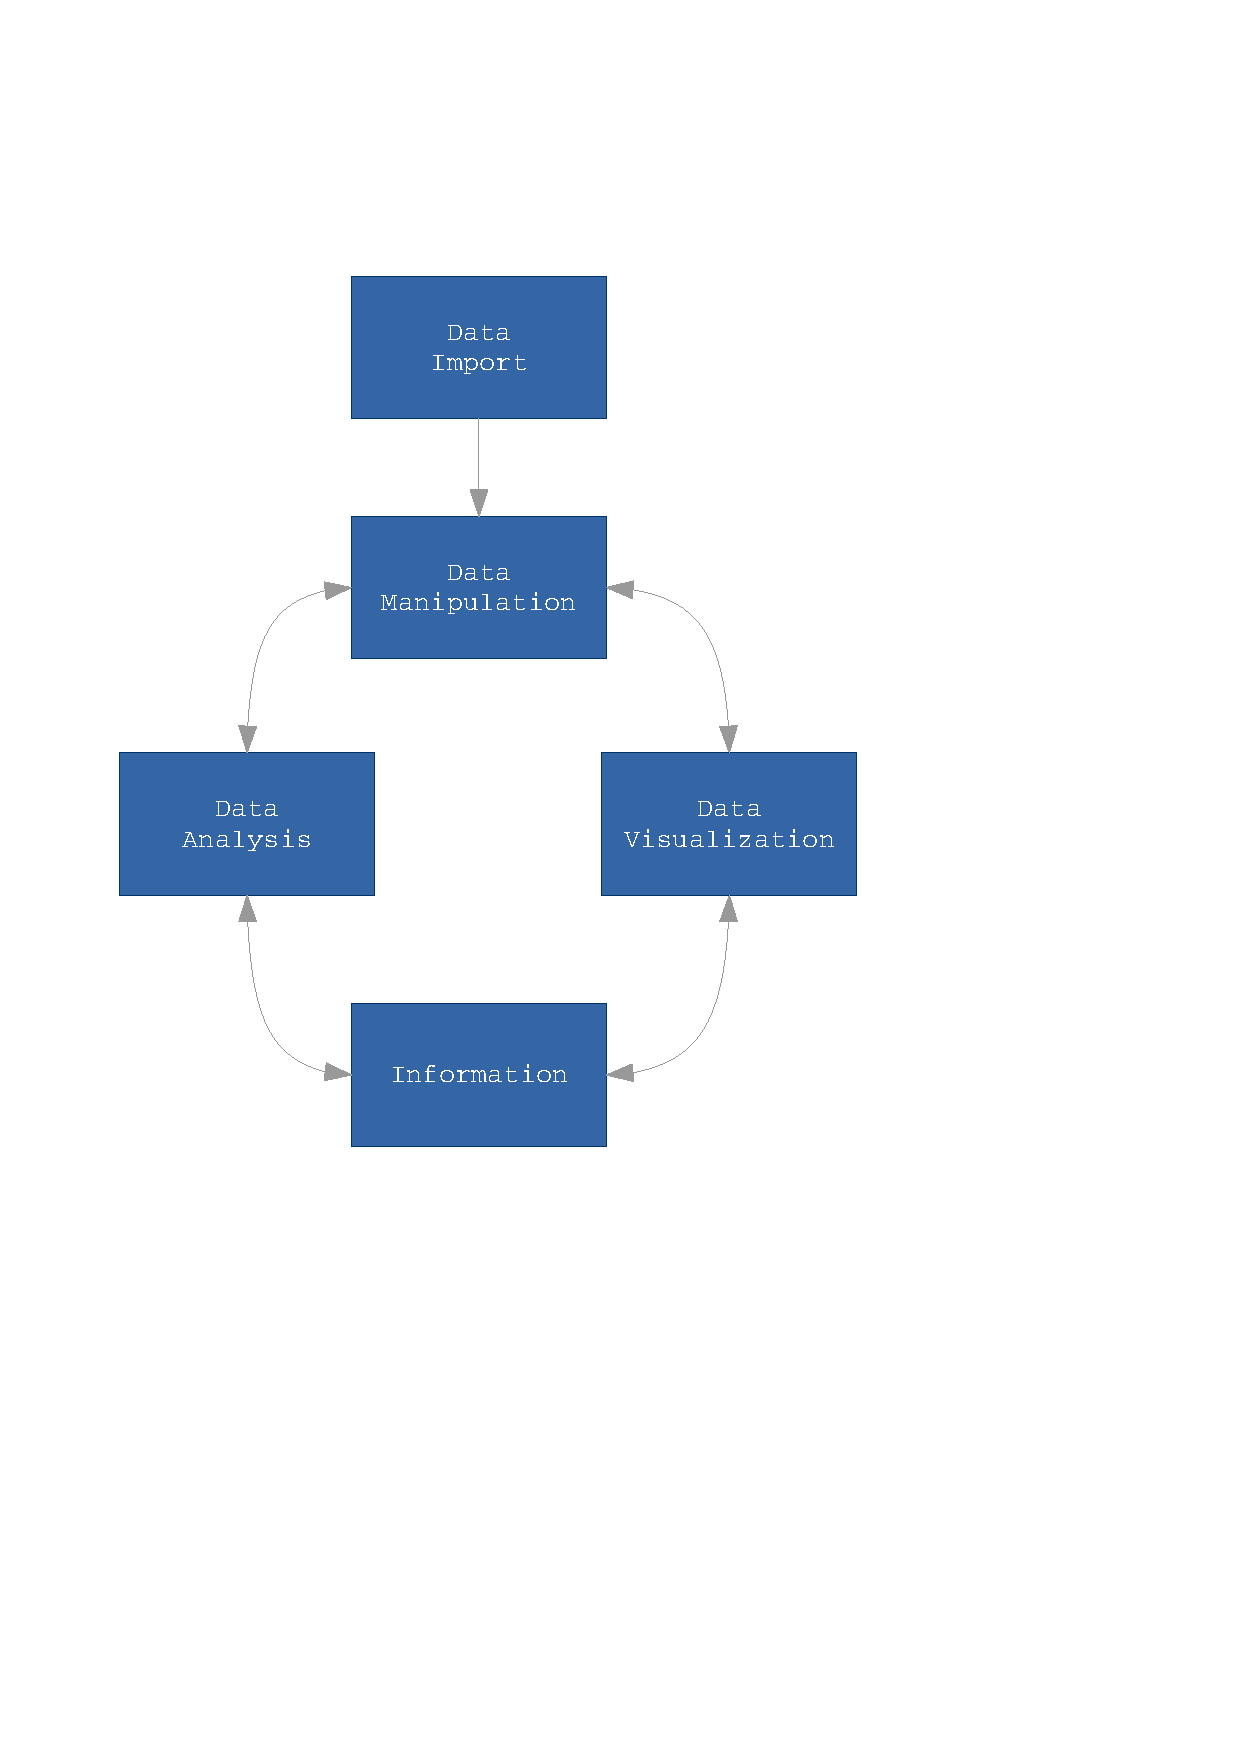
\includegraphics[width=3.6in]{images/flow}

This course offers the basics of R, and get an overview on methods for
data import, data manipulation, data visualization and data analysis.\\
You can download the course material here:
www.github.com/quantide/your-first-date-with-r/archive/master.zip

\clearpage

\section{Acknowledgements}\label{acknowledgements}

This web book is the result of several years of introductory R courses.
It contains work of my colleagues:

\begin{itemize}
\tightlist
\item
  Daniela Manzato, who wrote the first version of this book,
\item
  Enrico Pegoraro, who wrote chapters about statistical modeling,
\item
  Veronica Giro and Nicola Sturaro, which reviewed and reassembled all
  these materials.
\end{itemize}

\includegraphics[width=5.72in]{images/EF5C8766}

However, it would not have been possible without the sharing of
knowledge, information, ideas, doubts and even criticisms of many
individuals on the internet. I would like to extend my sincere thanks to
all of them.

I am grateful to Bill Venables and John Chambers for their publications
on R that provided solid foundations to my knowledge on this subject.
Moreover \href{http://www.statmethods.net/}{Quick R} often provides some
useful ready-to-cook recipe.

I would finally like to express my special gratitude to Hadley Wickham
for providing and sharing his research on the \texttt{R} packages:
\texttt{dplyr}, \texttt{ggplot2} and \texttt{readxl}. Without his
contribution, a part of this manual would never have been written.

I finally express my sincere excuses to all researchers and R
enthusiasts I have borrowed any knowledge from without mentioning them.
This was not intentional, simply I had not always tracked my sources. If
this is the case, please contact me directly and I will be more than
happy to include any appropriate reference in this manual.

Andrea Spanò,\\
Quantide s.r.l.

\chapter{R and a bit of history}\label{r-and-a-bit-of-history}

R is a programming environment for data analysis, graphics and
statistical computing. The R language is widely used among statisticians
for developing statistical software and data analysis. R was born as a
dialect of the S language, which is a statistical programming language
developed by John Chambers and others in Bell Laboratories. R is also
very close to S-PLUS, which is a commercial implementation of the S
programming language, sold by Insightful Corporation.

Let us see a bit of history.

\section{S and a bit of history}\label{s-and-a-bit-of-history}

S is a statistical programming language developed by John Chambers and
others in Bell Laboratories. The aim of the language, as expressed by
John Chambers, is ``to turn ideas into software, quickly and
faithfully''.

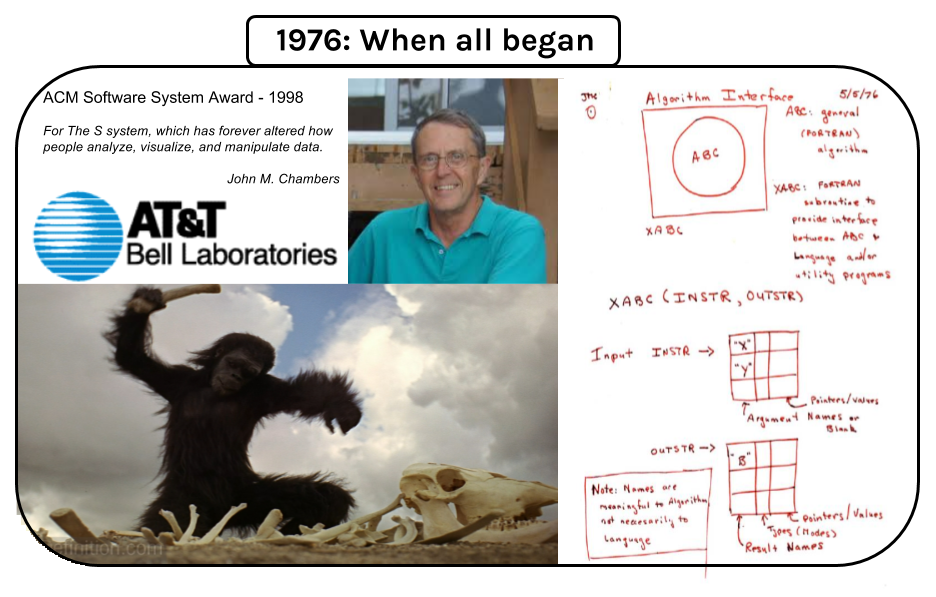
\includegraphics[width=6.24in]{images/s-rev}

A bit of history:

\begin{itemize}
\tightlist
\item
  1976: the first version of S is developed as an internal statistical
  analysis environment. It is originally implemented as Fortran
  libraries.
\item
  1980: the first version of S is distributed outside of Bell
  Laboratories. In 1981, source version is made available.
\item
  1984: Richard A. Becker and John M. Chambers, ``S. An Interactive
  Environment for Data Analysis and Graphics''. (Brown Book). Historical
  interest only.
\item
  1988: Richard A. Becker, John M. Chambers and Allan R. Wilks, ``The
  New S Language''. London: Chapman \& Hall. (Blue Book). It introduces
  what is now known as S version 2. The system is rewritten in C and
  begins to resemble the system that we have today.
\item
  1992: John M. Chambers and Trevor J. Hastie, ``Statistical Models in
  S''. (White Book). It introduces S version 3, often abbreviated S3,
  which adds structures to facilitate statistical modeling in S.
\item
  1998: John M. Chambers, ``Programming with Data''. (Green Book). It
  introduces S version 4, often abbreviated S4, which provides advanced
  object-oriented features. S4 classes differ markedly from S3 classes.
\end{itemize}

The S language itself has not changed dramatically since 1998.

\section{S-PLUS and a bit of history}\label{s-plus-and-a-bit-of-history}

S-PLUS is a commercial implementation of the S programming language.
S-PLUS provides a number of fancy features (GUIs, mostly) on top of it,
hence the ``PLUS''.


\includegraphics[width=6.16in]{images/s+}

A bit of history:

\begin{itemize}
\tightlist
\item
  1988: S-PLUS is first produced by a Seattle-based start-up company
  called Statistical Sciences, Inc. The founder and sole owner is R.
  Douglas Martin, professor of statistics at the University of
  Washington, Seattle.
\item
  1993: Statistical Sciences, Inc. acquires the exclusive license to
  distribute S and merges with MathSoft.
\item
  2001: MathSoft sells its Cambridge-based Engineering and Education
  Products Division (EEPD). It changes name to Insightful Corporation.
\item
  2004: Insightful purchases the S language from Lucent Technologies for
  \$2 million.
\item
  2008: TIBCO acquires Insightful Corporation.
\end{itemize}

\section{A bit of R history}\label{a-bit-of-r-history}

R was initially developed in early 90s by Robert Gentleman and Ross
Ihaka at the Department of Statistics of the University of Auckland, New
Zealand. The R name is partly based on the (first) names of the first
two R authors (Robert Gentleman and Ross Ihaka), and partly a play on
the name of S.

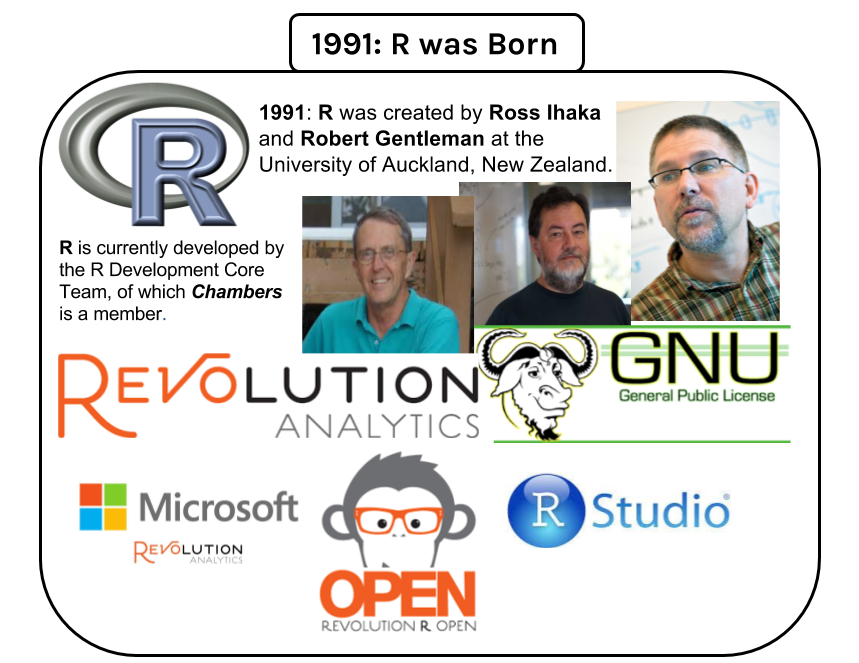
\includegraphics[width=5.73in]{images/r}

A bit of history:

\begin{itemize}
\tightlist
\item
  1991: R was created by Ross Ihaka and Robert Gentleman at the
  University of Auckland, New Zeland.
\item
  1993: First announcement of R to the public.
\item
  1995: Martin Maechler convinces Ross Ihaka and Robert Gentleman to use
  the GNU General Public License to make R free software.
\item
  1997: The R Development Core Team is formed. The team controls the
  source code for R.
\item
  2000: R version 1.0.0 released. Developers consider R stable enough
  for production use.
\item
  2004: R version 2.0.0 released. Introduced lazy loading, which enables
  fast loading of data with minimal expense of system memory.
\item
  2013: R version 3.0.0 released. Introduced long vectors.
\end{itemize}

While R is an open source project supported by the community developing
it, some companies strive to provide commercial support and/or
extensions for their customers. R history is intertwined with that of
its commercial support:

\begin{itemize}
\tightlist
\item
  2007: Revolution Analytics was founded to provide commercial support
  for Revolution R, the distribution of R developed by Revolution
  Analytics which also includes components developed by the company.
\item
  2010: RStudio was founded. It is a company that develops free and open
  tools for the R community.
\item
  2014: Microsoft Corporation starts the release of Microsoft R Open, an
  enhanced distribution of R, formerly known as Revolution R Open (RRO).
\item
  2015: Microsoft Corporation completed the acquisition of Revolution
  Analytics.
\end{itemize}

We will deepen the commercial support tools mentioned in \emph{Online
Resources} chapter.

\section{Why R?}\label{why-r}

In December 2016, R is in 17th place of TIOBE Programming Community
Index (\href{http://www.tiobe.com/tiobe-index/}{www.tiobe.com}), that is
an indicator of the popularity of programming languages. R is above SAS
that is in 22th place.

R is the leading analytics tools for data science used by respondents to
the Rexer Analytics Survey in 2015:

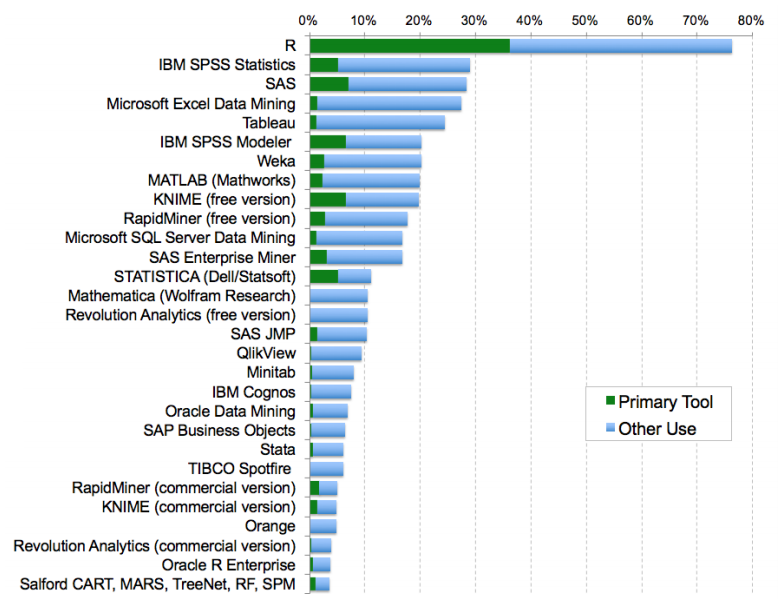
\includegraphics[width=5.23in]{images/r-popularity}

Moreover, the number of companies using R is grown all over the world:

\begin{figure}
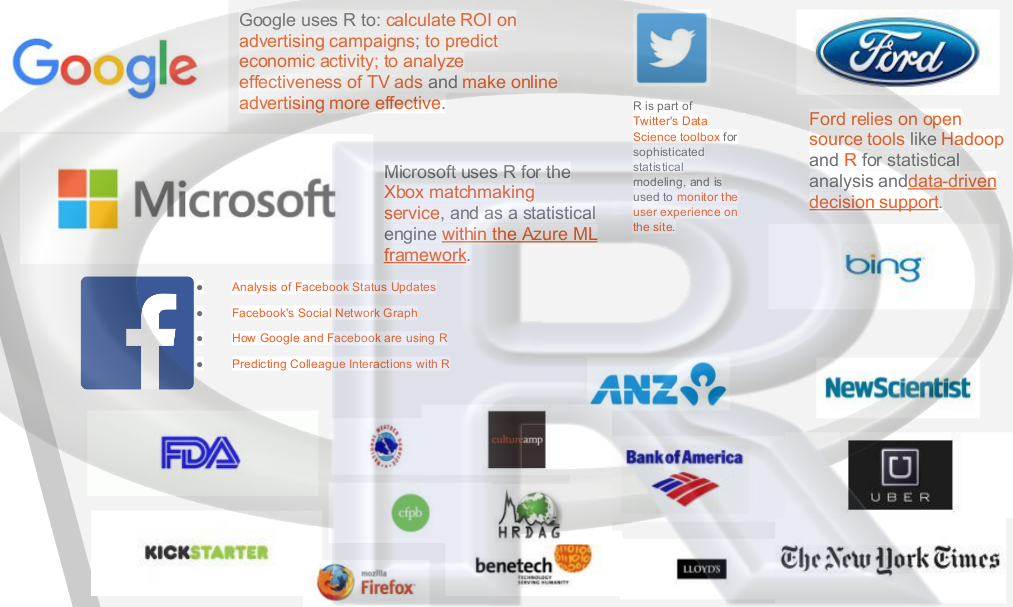
\includegraphics[width=6.75in]{images/company-using-r} \caption{Source: blog.revolutionanalytics.com}\label{fig:g6}
\end{figure}

\chapter{Online Resources}\label{online-resources}

R strength is its community, which is distributed and keeps growing all
over the World!

\begin{figure}[htbp]
\centering
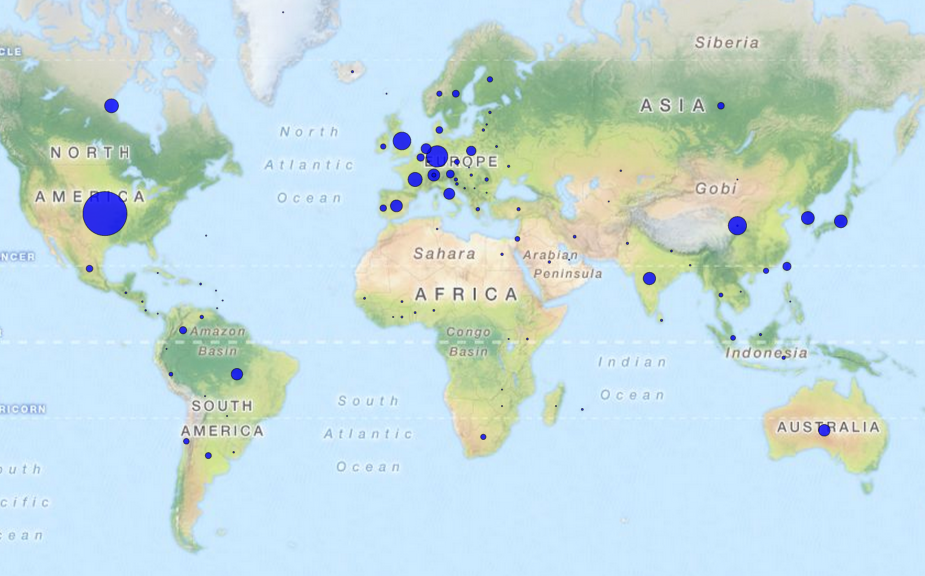
\includegraphics{./images/r-users-distribution.png}
\caption{}
\end{figure}

Thanks to its community, R can boast a wide variety of online resources,
free and otherwise, to learn more about it, ranging from websites, blogs
and commercial support tools.

Let us have a look at the most important.

\section{The R-project and R Licence}\label{the-r-project-and-r-licence}

R is supported by a wide community of academic users, professors,
companies and developers. This community composes the so-called
``R-project''. The ``R-project'' is supported by the ``R Foundation''.
The R Foundation is a not for profit organisation, working in the public
interest.

R is an official part of the Free Software Foundation's GNU project. The
R Foundation has similar goals to other open source software foundations
like the Apache Foundation or the GNOME Foundation. R is free and open
source software. It is released under the GPL (version 2) licence.

R is free:

\begin{itemize}
\tightlist
\item
  you can have R without paying for it (freeware);
\item
  you can copy and re-use the software (free software);
\item
  you can access source code and modify it (open source).
\end{itemize}

\subsection{R-project Website}\label{r-project-website}

The R-project website
\href{http://www.r-project.org/}{(www.r-project.org)} is the starting
point for R materials.

The website contains:

\begin{itemize}
\tightlist
\item
  the software and packages;
\item
  the search engine interface (the same queries can be submitted with
  the RSiteSearch (`query') function within R);
\item
  the on-line documentation both in HTML and in PDF format. The HTML
  version can be accessed with the \texttt{help.start()} function within
  R;
\item
  the R Journal. The R Journal is the open access, refereed journal of
  the R project. It features short to medium length articles covering
  topics that might be of interest to users or developers of R;
\item
  the interface to the mailing list;
\item
  the wiki, suggested books and many others.
\end{itemize}

The on-line documentation includes the following manuals. These manuals
have been written by the R Development Core Team itself and contain
precious information.

\begin{itemize}
\tightlist
\item
  \emph{An Introduction to R} gives an introduction to the language and
  how to use R for doing statistical analysis and graphics.
\item
  \emph{Writing R Extensions} covers how to create your own packages,
  write R help files, and the foreign language (C, C++, Fortran,
  \ldots{}) interfaces.
\item
  \emph{R Data Import/Export} describes the import and export facilities
  available either in R itself or via packages which are available from
  CRAN.
\item
  \emph{R Installation and Administration}.
\end{itemize}

Other manuals and tutorials provided by R users can be downloaded from
the R-project website
\href{http://cran.r-project.org/other-docs.html}{(cran.r-project.org/other-docs.html)}.

Mailing lists is the most important tool to contact the R community.
Mailing lists can be accessed from the R-project website
\href{http://www.r-project.org/mail.html}{(www.r-project.org/mail.html)}.

There are five general mailing lists devoted to R:

\begin{itemize}
\tightlist
\item
  \emph{R-announce}: This list is for major announcements about the
  development of R and the availability of new code.
\item
  \emph{R-packages}: This list is for announcements as well, usually on
  the availability of new or enhanced contributed packages (on CRAN,
  typically).
\item
  \emph{R-help}: The ``main'' R mailing list, for discussion about
  problems and solutions using R, announcements about the availability
  of new functionality for R and documentation of R, comparison and
  compatibility with S-plus, and for the posting of nice examples and
  benchmarks.
\item
  \emph{R-devel}: This list is intended for questions and discussion
  about code development in R.
\item
  \emph{R-package-devel}: This list is to get help about package
  development in R.
\end{itemize}

\section{Other Online Resources}\label{other-online-resources}

It is very difficult estimate how many sites about R are on-line.
However, Google returns 224.000.000 sites searching ``R stat blog''.
Also if only the 0.1\% of these sites talk about R, it means almost
220.000 sites about R.

R-bloggers \href{http://www.r-bloggers.com/}{(www.r-bloggers.com)} is a
blog aggregator of content collected from bloggers who write about R.
R-bloggers contains R news and tutorials contributed by hundreds of R
bloggers.

We suggest you to visit MilanoR
\href{http://www.milanor.net/}{(www.milanor.net)}, which is the blog of
R users in the Milan Area. Its aim is to exchange knowledge, learn and
share tricks and techniques and provide R beginners with an opportunity
to meet more experienced users.

Other useful websites about R are:

\begin{itemize}
\tightlist
\item
  Stack Overflow
  \href{http://stackoverflow.com/}{(www.stackoverflow.com)} is a website
  that features questions and answers on a wide range of topics in
  computer programming, among which r.
\item
  Quick-R \href{http://www.statmethods.net/}{(www.statmethods.net)} is a
  useful on-line guide to R. It provides many examples and useful tips.
\item
  R seek \href{http://rseek.org/}{(rseek.org)} uses Google to search in
  a selected list of websites about R.
\end{itemize}

\subsection{R Commercial Support}\label{r-commercial-support}

While R is an open source project supported by the community developing
it, some companies strive to provide commercial support and/or
extensions for their customers.

\subsubsection{Microsoft Corporation}\label{microsoft-corporation}

Microsoft Corporation provides Microsoft R Open
\href{https://mran.microsoft.com/open/}{www.mran.microsoft.com/open}, an
enhanced distribution of R, formerly known as Revolution R Open (RRO).
It is a complete open source platform for statistical analysis and data
science. The current version, Microsoft R Open 3.3.2, is based on (and
100\% compatible with) R-3.3.2 and is therefore fully compatibility with
all packages, scripts and applications that work with that version of R.
It includes additional capabilities for improved performance,
reproducibility, as well as support for Windows and Linux-based
platforms. Like R, Microsoft R Open is open source and free to download,
use, and share. It is available for Windows, Linux and Mac Os operative
systems and you can download it
\href{https://mran.microsoft.com/download/}{here}.

\subsubsection{RStudio, Inc.}\label{rstudio-inc.}

RStudio, Inc. \href{http://www.rstudio.com/}{(www.rstudio.com)} is a
company that develops free and open tools for the R community, inspired
by the innovations of R users in science, education, and industry. These
include the RStudio development environment as well as the
\texttt{shiny}, \texttt{ggvis}, and \texttt{dplyr} packages (among many
others). RStudio was founded around December 2010 by JJ Allaire, creator
of the programming language ColdFusion. Hadley Wickham is the Chief
Scientist at RStudio. RStudio has a mission to provide the most widely
used open source and enterprise-ready professional software for the R
statistical computing environment. These tools will further the cause of
expanding the use of R and the field of data science. It also offers
open source and enterprise ready tools for the R computing environment.
The flagship product of the RStudio team is an Integrated Development
Environment (IDE) which makes it easy for analysts, scientists, data
scientists and quants to perform their analyses. It also offer Shiny: a
platform that allows you to take those analyses and share them with your
team/organization by creating interactive web applications.

\chapter{R and R-Studio installation and
configuration}\label{r-and-r-studio-installation-and-configuration}

\section{Installing and Updating R}\label{installing-and-updating-r}

\subsection{Design of the R System}\label{design-of-the-r-system}

The R system is divided into two conceptual parts:

\begin{enumerate}
\def\labelenumi{\arabic{enumi}.}
\tightlist
\item
  The ``base'' R system that you download from CRAN.
\item
  Everything else.
\end{enumerate}

R functionality is divided into a number of packages. The ``base'' R
system contains, among other things, the \emph{base} package which is
required to run R and contains the most fundamental functions. The
``base'' system contains also some other packages. Furthermore, every R
installation contains ``recommended'' packages, that are not necessarily
maintained by R Core.

``Everything else'' point out CRAN ``contributed'' packages and packages
that are not on CRAN. This does not mean that these packages are
necessarily of lesser quality than the above, e.g., many contributed
packages on CRAN are written and maintained by R Core members. The goal
is simply to try to keep the base distribution as lean as possible.
Beyond CRAN, many packages are avalaible in BioConductor project or in
Github repositories.

\clearpage

\subsection{Installing R}\label{installing-r}

R is available for Windows, Mac Os and Linux.

The base R can be downloaded from the Comprehensive R Archive Network
(CRAN) website. The CRAN is a collection of sites which carry identical
material, consisting of the R distribution(s), the contributed
extensions, documentation for R, and binaries.

Go to \href{http://www.r-project.org/}{www.r-project.org}. Here you can
read about R and see what's new in the latest version.

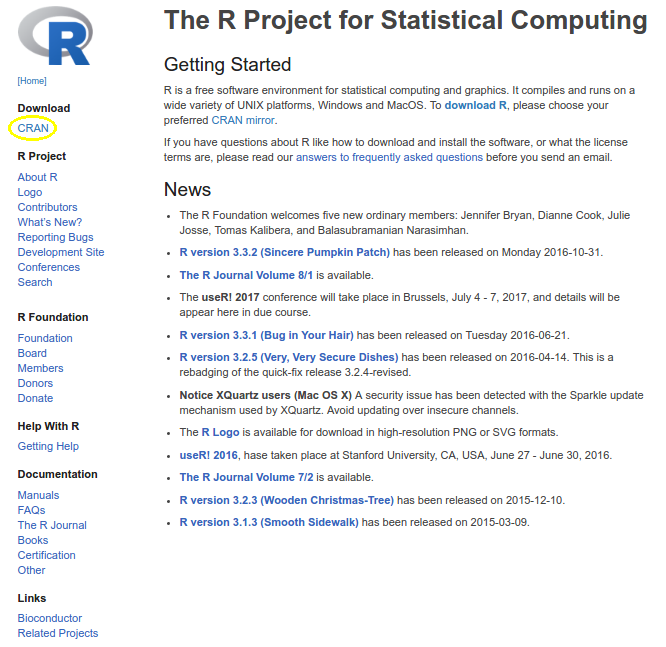
\includegraphics[width=4.44in]{./images/r-project}

Click on CRAN under Download in the left list. That'll take you to a
list of servers (mirrors) in different countries where you can download
R.

Now you can choose what operative system you have. Choose within the
upper box with \emph{Download and Install R}. The box contains
\emph{Precompiled binary distributions}; sounds complicated, but means
that the program is ready to use, with installation program and all.

Windows users click on ``base'' and then click \emph{Download R X.X.X
for Windows}.

Mac users click on \emph{R-X.X.X.pkg (latest version)}.

Linux users find download files and installation instructions for their
Linux distribution in the website.

X.X.X identify the current version of R. In December 2016, the current
version is the 3.3.2.

To install R, Windows and Mac users must just double click on the file
and follow the installation instructions.

Linux users can download and install R using the precompiled R binary
for their distribution. Alternatively, experienced Linux users can
compile R from sources. Currently, precompiled R binary are available
for Debian, Ubuntu, Suse and RedHat.

The Figure \protect\hyperlink{fig:ssFirsttry}{Screenshot of a first try
with R} shows a first try with R, just after installation.

\hypertarget{fig:ssFirsttry}{}
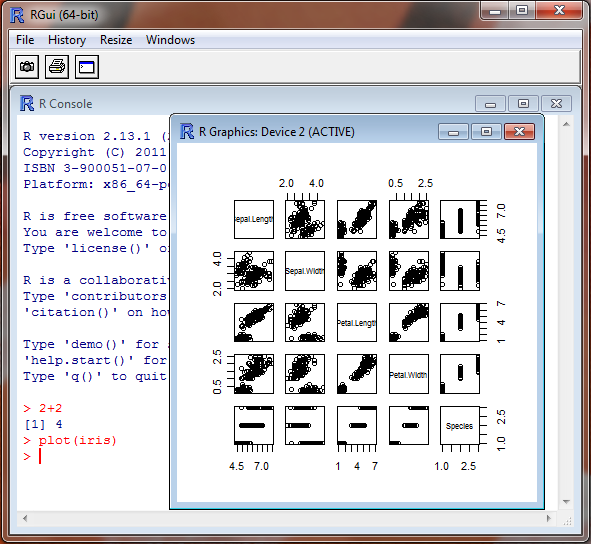
\includegraphics[width=3.94in]{./images/RfirstPlot}

\subsection{Updating R}\label{updating-r}

In Windows and Mac, there is not an automatic way to update R. Two or
more versions of R can coexist in the same machine, so a newer release
of R can be installed beside the old release. Unfortunately, packages
must be re-installed in the ``new'' R version. A copy-and-paste of
package files from the directory containing the packages of the ``old''
R version to the directory containing the packages of the ``new'' R
version may be useful when many packages are installed. Within R, the
\texttt{.Library} variable shows the directory containing the packages.
After the copy-and-paste, packages of the ``new'' R version should be
updated.

In Linux, usually one R version at time can be installed. R can be
updated following the instructions in the CRAN website.

\section{Graphical User Interfaces}\label{graphical-user-interfaces}

\subsection{R Default Interfaces}\label{r-default-interfaces}

R is provided with a Command Line Interface (CLI), which is the
preferred user interface for power users because it allows direct
control on calculations and it is flexible. However, good knowledge of
the language is required. CLI is thus intimidating for beginners.

R is available for many different operative systems so it does not
provide the same graphical interface. When you use the R program
interactively, it issues a prompt when it expects input commands. The
default prompt is `\textgreater{}'. In Windows, RGui is the default GUI.
Inside RGui there is the RConsole window. In Macintosh, RConsole is the
default GUI. In Linux, R does not provide any graphical interface by
default and it can be used through CLI.

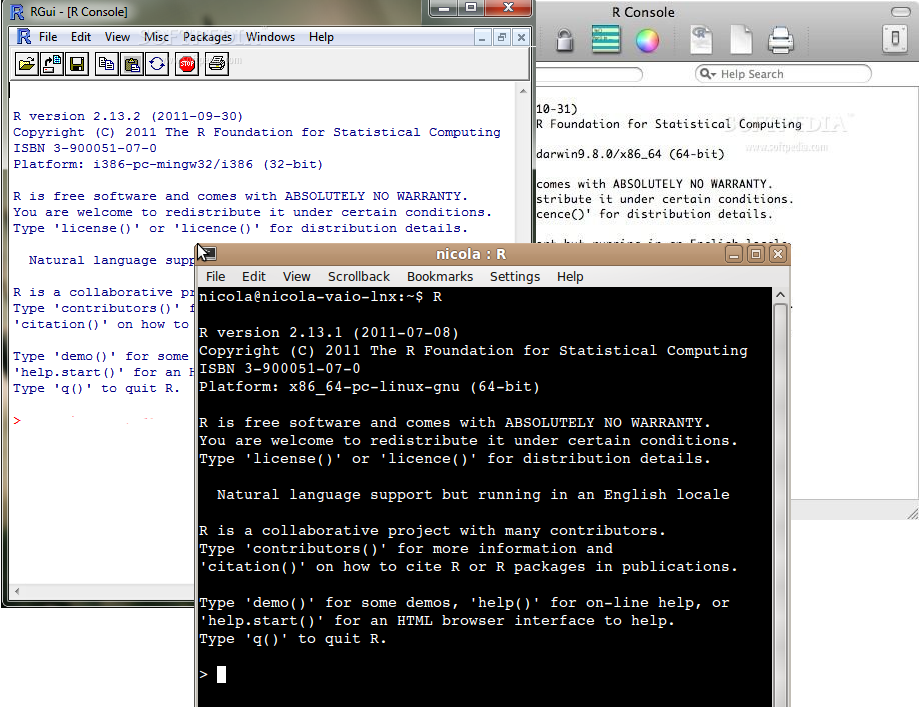
\includegraphics[width=6.13in]{./images/ssDefaultGui}

\clearpage

\subsection{RStudio}\label{rstudio}

\textbf{RStudio} \href{http://www.rstudio.org/}{(www.rstudio.org)} is a
free and open source multi-platform integrated development environment
(IDE) for R. It provides syntax highlighting, code completion and smart
indentation. Moreover, it executes R code directly from the source
editor and it manages easily multiple working directories using
projects. It provides:

\begin{itemize}
\tightlist
\item
  workspace browser and data viewer;
\item
  plot history, zooming, and flexible image and PDF export;
\item
  integrated R help and documentation;
\item
  Sweave authoring including one-click PDF preview;
\item
  searchable command history.
\end{itemize}

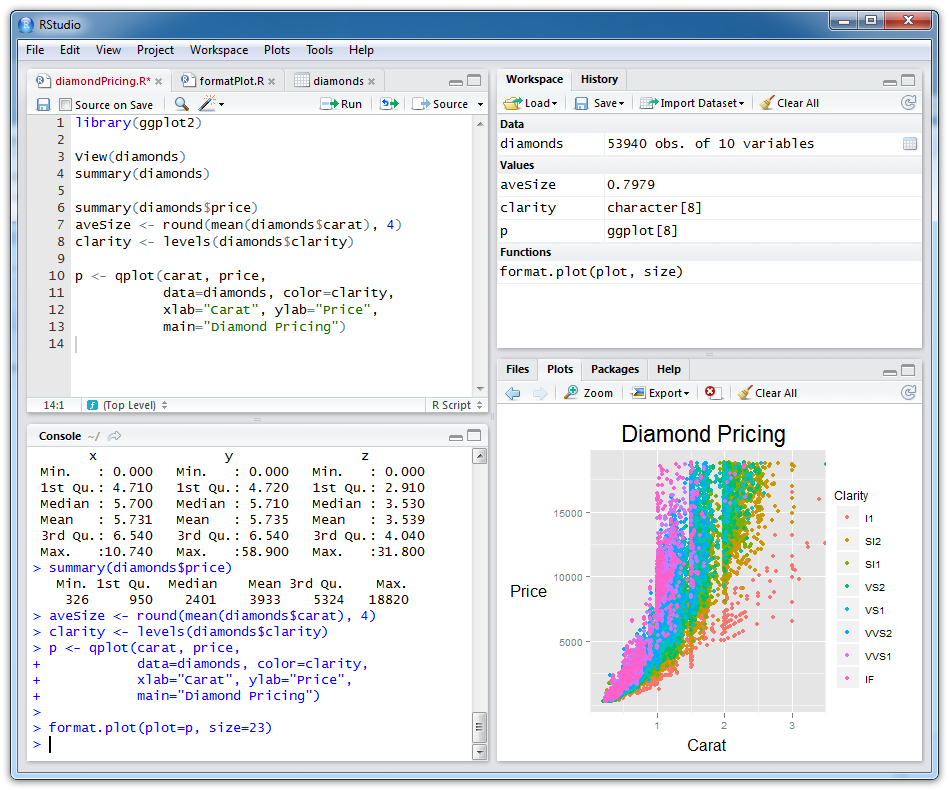
\includegraphics[width=6.33in]{./images/ssGuiRstudio}

\subsection{Installing RStudio}\label{installing-rstudio}

RStudio is available for Windows, Mac Os and Linux and you can install
it from its website \href{http://www.rstudio.org/}{(www.rstudio.org)},
clicking on \emph{Download RStudio}. Next, click \emph{Download RStudio
Desktop}. At this stage, click the link to the version of RStudio
appropriate for your system in \emph{Installers for Supported Platforms}
section, which downloads RStudio to your computer. Run the installation
file and RStudio will be installed on your system.

\section{R Packages}\label{r-packages}

\subsection{Installing R Packages}\label{installing-r-packages}

R functions are collected in packages. Packages that are not contained
in the ``base'' R systems can be downloaded from the CRAN website. A
list of R packages accompanied by a brief description can be found on
the CRAN website where there are more than 9500 packages available. Many
of these packages are very useful; however, there are some packages in
prerelease, incomplete packages, ``abandoned'' packages (i.e.~not more
updated) and/or packages containing functions with errors or
compatibility troubles.

This is the R package universe!

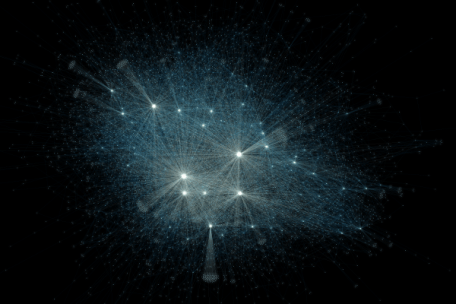
\includegraphics[width=3.04in]{./images/r-packages-universe}

The simple way to install an R package is through the
\texttt{install.packages()} function, directly from R. In Linux, R must
be executed as administrator to install a package. Installation must be
executed before the first use of a library.

When a function of a package that is not contained in the ``base'' R
systems is required, the package must be loaded. The
\texttt{require(pkg)} function load the \emph{pkg} package.

\subsection{Updating R Packages}\label{updating-r-packages}

R packages can be updated typing \texttt{update.packages()} within R. In
Linux, R must be executed as administrator to update a package. Packages
should be updated regularly.

\chapter{Your first R session}\label{your-first-r-session}

\section{Aritmetic with R}\label{aritmetic-with-r}

Start the R system, the cursor is waiting for you to type in some R
commands. For example, use R as a simple calculator:

\begin{Shaded}
\begin{Highlighting}[]
\DecValTok{6} \NormalTok{+}\StringTok{ }\DecValTok{3}
\end{Highlighting}
\end{Shaded}

\begin{verbatim}
## [1] 9
\end{verbatim}

\begin{Shaded}
\begin{Highlighting}[]
\DecValTok{5} \NormalTok{-}\StringTok{ }\DecValTok{9}
\end{Highlighting}
\end{Shaded}

\begin{verbatim}
## [1] -4
\end{verbatim}

\begin{Shaded}
\begin{Highlighting}[]
\DecValTok{4} \NormalTok{*}\StringTok{ }\DecValTok{6}
\end{Highlighting}
\end{Shaded}

\begin{verbatim}
## [1] 24
\end{verbatim}

\begin{Shaded}
\begin{Highlighting}[]
\DecValTok{8} \NormalTok{/}\StringTok{ }\DecValTok{3}
\end{Highlighting}
\end{Shaded}

\begin{verbatim}
## [1] 2.666667
\end{verbatim}

\begin{Shaded}
\begin{Highlighting}[]
\DecValTok{5} \NormalTok{^}\StringTok{ }\DecValTok{2}
\end{Highlighting}
\end{Shaded}

\begin{verbatim}
## [1] 25
\end{verbatim}

\begin{Shaded}
\begin{Highlighting}[]
\NormalTok{(}\DecValTok{1} \NormalTok{+}\StringTok{ }\FloatTok{0.05}\NormalTok{)^}\DecValTok{8}
\end{Highlighting}
\end{Shaded}

\begin{verbatim}
## [1] 1.477455
\end{verbatim}

\begin{Shaded}
\begin{Highlighting}[]
\KeywordTok{exp}\NormalTok{(}\DecValTok{3}\NormalTok{)}
\end{Highlighting}
\end{Shaded}

\begin{verbatim}
## [1] 20.08554
\end{verbatim}

\begin{Shaded}
\begin{Highlighting}[]
\KeywordTok{log}\NormalTok{(}\DecValTok{14}\NormalTok{)}
\end{Highlighting}
\end{Shaded}

\begin{verbatim}
## [1] 2.639057
\end{verbatim}

\begin{Shaded}
\begin{Highlighting}[]
\FloatTok{23.76} \NormalTok{*}\StringTok{ }\KeywordTok{log}\NormalTok{(}\DecValTok{8}\NormalTok{)/(}\DecValTok{23} \NormalTok{+}\StringTok{ }\KeywordTok{atan}\NormalTok{(}\DecValTok{9}\NormalTok{))}
\end{Highlighting}
\end{Shaded}

\begin{verbatim}
## [1] 2.01992
\end{verbatim}

\section{Assignment}\label{assignment}

Results of calculations can be stored in objects using the assignment
operator:

\begin{Shaded}
\begin{Highlighting}[]
\NormalTok{x <-}\StringTok{ }\KeywordTok{log}\NormalTok{(}\DecValTok{14}\NormalTok{)}
\NormalTok{y <-}\StringTok{ }\FloatTok{23.76} \NormalTok{*}\StringTok{ }\KeywordTok{log}\NormalTok{(}\DecValTok{8}\NormalTok{)/(}\DecValTok{23} \NormalTok{+}\StringTok{ }\KeywordTok{atan}\NormalTok{(}\DecValTok{9}\NormalTok{))}
\end{Highlighting}
\end{Shaded}

To print the object just enter the name of the object or use
\texttt{print()} function.

\begin{Shaded}
\begin{Highlighting}[]
\NormalTok{x}
\end{Highlighting}
\end{Shaded}

\begin{verbatim}
## [1] 2.639057
\end{verbatim}

\begin{Shaded}
\begin{Highlighting}[]
\KeywordTok{print}\NormalTok{(y)}
\end{Highlighting}
\end{Shaded}

\begin{verbatim}
## [1] 2.01992
\end{verbatim}

These objects can then be used in other calculations.

\begin{Shaded}
\begin{Highlighting}[]
\NormalTok{z <-}\StringTok{ }\NormalTok{x +}\StringTok{ }\NormalTok{y}
\NormalTok{z}
\end{Highlighting}
\end{Shaded}

\begin{verbatim}
## [1] 4.658978
\end{verbatim}

\section{The R Workspace}\label{the-r-workspace}

The workspace is your current R working environment and includes any
user-defined objects. It is also known as global environment.

\subsection{Objects listing}\label{objects-listing}

Objects created during an R session are hold in memory. To list the
objects in the current R session, the function \texttt{ls()} or the
function \texttt{objects()} may be used.

\begin{Shaded}
\begin{Highlighting}[]
\KeywordTok{ls}\NormalTok{()}
\end{Highlighting}
\end{Shaded}

\begin{verbatim}
## [1] "x" "y" "z"
\end{verbatim}

\begin{Shaded}
\begin{Highlighting}[]
\KeywordTok{objects}\NormalTok{()}
\end{Highlighting}
\end{Shaded}

\begin{verbatim}
## [1] "x" "y" "z"
\end{verbatim}

\subsection{Removing objects}\label{removing-objects}

If a value to an object that already exists is assigned then the
contents of the object will be overwritten with the new value (without a
warning!). The function \texttt{rm()} ought be used to remove one or
more objects from your session.

\begin{Shaded}
\begin{Highlighting}[]
\KeywordTok{rm}\NormalTok{(x)}
\KeywordTok{ls}\NormalTok{()}
\end{Highlighting}
\end{Shaded}

\begin{verbatim}
## [1] "y" "z"
\end{verbatim}

\section{R help}\label{r-help}

Within R, the following functions provide help about R itself:

\begin{itemize}
\tightlist
\item
  The HTML version of R's online documentation can be printed on-screen
  by typing \texttt{help.start()};
\item
  Online documentation for most of the functions and variables in R can
  be printed on-screen by typing \texttt{help(name)} (or
  \texttt{?name}), where \emph{name} is the name of the topic help is
  sought for;
\item
  Online documentation for finding help pages on a vague topic can be
  printed on-screen by typing
  \texttt{help.search(\textquotesingle{}topic\textquotesingle{})};
\item
  A list of function containing \emph{topic} in the name can be printed
  on-screen by typing
  \texttt{apropos(\textquotesingle{}topic\textquotesingle{})};
\item
  A research in the website can be performed by typing
  \texttt{RSiteSearch(\textquotesingle{}query\textquotesingle{})}, where
  \emph{query} is the search query.
\end{itemize}

For example, to get help about the \texttt{mean()} function, the
\texttt{help()} function can be used.

\begin{Shaded}
\begin{Highlighting}[]
\KeywordTok{help}\NormalTok{(mean)}
\end{Highlighting}
\end{Shaded}

The \texttt{help()} function can be called using the \texttt{?}.

\begin{Shaded}
\begin{Highlighting}[]
\NormalTok{?mean}
\end{Highlighting}
\end{Shaded}

To get a list of functions concerning the mean, the
\texttt{help.search()} function can be used.

\begin{Shaded}
\begin{Highlighting}[]
\KeywordTok{help.search}\NormalTok{(}\StringTok{"mean"}\NormalTok{)}
\end{Highlighting}
\end{Shaded}

To get a list of function containing ``mean'' in the name, the
\texttt{apropos()} function can be used.

\begin{Shaded}
\begin{Highlighting}[]
\KeywordTok{apropos}\NormalTok{(}\StringTok{"mean"}\NormalTok{)}
\end{Highlighting}
\end{Shaded}

\chapter{Data Objects}\label{data-objects}

\section{Data frames}\label{data-frames}

\textbf{Data frames} are the primary data structure in R. A data frame
is a table, in which each column contains measurements on one variable,
and each row contains one case. Each row may be treated as a single
observation of multiple ``variables''.

\begin{Shaded}
\begin{Highlighting}[]
\NormalTok{df <-}\StringTok{ }\KeywordTok{data.frame}\NormalTok{(}
  \DataTypeTok{name =} \KeywordTok{c}\NormalTok{(}\StringTok{"James"}\NormalTok{, }\StringTok{"Stevie"}\NormalTok{, }\StringTok{"Otis"}\NormalTok{, }\StringTok{"Bob"}\NormalTok{, }\StringTok{"Levon"}\NormalTok{, }\StringTok{"Patti"}\NormalTok{, }\StringTok{"Karen"}\NormalTok{), }
  \DataTypeTok{height =} \KeywordTok{c}\NormalTok{(}\DecValTok{180}\NormalTok{, }\DecValTok{170}\NormalTok{, }\DecValTok{175}\NormalTok{, }\DecValTok{190}\NormalTok{, }\DecValTok{168}\NormalTok{, }\DecValTok{160}\NormalTok{, }\DecValTok{165}\NormalTok{), }
  \DataTypeTok{graduated =} \KeywordTok{c}\NormalTok{(}\OtherTok{TRUE}\NormalTok{, }\OtherTok{TRUE}\NormalTok{, }\OtherTok{FALSE}\NormalTok{, }\OtherTok{FALSE}\NormalTok{, }\OtherTok{FALSE}\NormalTok{, }\OtherTok{TRUE}\NormalTok{, }\OtherTok{TRUE}\NormalTok{),}
  \DataTypeTok{gender =} \KeywordTok{factor}\NormalTok{(}\KeywordTok{c}\NormalTok{(}\StringTok{"M"}\NormalTok{, }\StringTok{"M"}\NormalTok{, }\StringTok{"M"}\NormalTok{, }\StringTok{"M"}\NormalTok{, }\StringTok{"M"}\NormalTok{, }\StringTok{"F"}\NormalTok{, }\StringTok{"F"}\NormalTok{)), }
  \DataTypeTok{stringsAsFactors =} \OtherTok{FALSE}\NormalTok{)}
\NormalTok{df}
\end{Highlighting}
\end{Shaded}

\begin{verbatim}
##     name height graduated gender
## 1  James    180      TRUE      M
## 2 Stevie    170      TRUE      M
## 3   Otis    175     FALSE      M
## 4    Bob    190     FALSE      M
## 5  Levon    168     FALSE      M
## 6  Patti    160      TRUE      F
## 7  Karen    165      TRUE      F
\end{verbatim}

Technically, in R a data frame is a list of column vectors that can be
of various types, but that have to be of the same length. A
\textbf{vector} is a ``primitive'' data object, it is a sequence of data
elements of the same basic type:

\begin{itemize}
\tightlist
\item
  numeric
\item
  character
\item
  logical
\end{itemize}

\begin{Shaded}
\begin{Highlighting}[]
\CommentTok{# Numeric vector}
\NormalTok{height <-}\StringTok{ }\KeywordTok{c}\NormalTok{(}\DecValTok{180}\NormalTok{, }\DecValTok{170}\NormalTok{, }\DecValTok{175}\NormalTok{, }\DecValTok{190}\NormalTok{, }\DecValTok{168}\NormalTok{, }\DecValTok{160}\NormalTok{, }\DecValTok{165}\NormalTok{)}
\NormalTok{height}
\end{Highlighting}
\end{Shaded}

\begin{verbatim}
## [1] 180 170 175 190 168 160 165
\end{verbatim}

\begin{Shaded}
\begin{Highlighting}[]
\CommentTok{# Character vector}
\NormalTok{name <-}\StringTok{ }\KeywordTok{c}\NormalTok{(}\StringTok{"James"}\NormalTok{, }\StringTok{"Stevie"}\NormalTok{, }\StringTok{"Otis"}\NormalTok{, }\StringTok{"Bob"}\NormalTok{, }\StringTok{"Levon"}\NormalTok{, }\StringTok{"Patti"}\NormalTok{, }\StringTok{"Karen"}\NormalTok{)}
\NormalTok{name}
\end{Highlighting}
\end{Shaded}

\begin{verbatim}
## [1] "James"  "Stevie" "Otis"   "Bob"    "Levon"  "Patti"  "Karen"
\end{verbatim}

\begin{Shaded}
\begin{Highlighting}[]
\CommentTok{# Logical vector}
\NormalTok{graduated <-}\StringTok{ }\KeywordTok{c}\NormalTok{(}\OtherTok{TRUE}\NormalTok{, }\OtherTok{TRUE}\NormalTok{, }\OtherTok{FALSE}\NormalTok{, }\OtherTok{FALSE}\NormalTok{, }\OtherTok{FALSE}\NormalTok{, }\OtherTok{TRUE}\NormalTok{, }\OtherTok{TRUE}\NormalTok{)}
\NormalTok{graduated}
\end{Highlighting}
\end{Shaded}

\begin{verbatim}
## [1]  TRUE  TRUE FALSE FALSE FALSE  TRUE  TRUE
\end{verbatim}

A data frame can include also \textbf{factors}, which are vector-like
objects used to specify a discrete classification (grouping) of the
components of other vectors of the same length. Factor variables are
categorical variables that can be either numeric or string variables.

\begin{Shaded}
\begin{Highlighting}[]
\CommentTok{# Factor variable}
\NormalTok{gender <-}\StringTok{ }\KeywordTok{factor}\NormalTok{(}\KeywordTok{c}\NormalTok{(}\StringTok{"M"}\NormalTok{, }\StringTok{"M"}\NormalTok{, }\StringTok{"M"}\NormalTok{, }\StringTok{"M"}\NormalTok{, }\StringTok{"M"}\NormalTok{, }\StringTok{"F"}\NormalTok{, }\StringTok{"F"}\NormalTok{))}
\NormalTok{gender}
\end{Highlighting}
\end{Shaded}

\begin{verbatim}
## [1] M M M M M F F
## Levels: F M
\end{verbatim}

A data frame is generated by \texttt{data.frame()} function. The vectors
composing the data frame can be defined inside the \texttt{data.frame()}
function itself (as seen in the first example) or can be defined outside
it. In the following example, we refer to the previously defined vectors
(\texttt{name}, \texttt{height}, \texttt{graduated}) and factor
(\texttt{gender}) to generate a dataframe:

\begin{Shaded}
\begin{Highlighting}[]
\NormalTok{df <-}\StringTok{ }\KeywordTok{data.frame}\NormalTok{(name, height, graduated, gender, }\DataTypeTok{stringsAsFactors =} \OtherTok{FALSE}\NormalTok{)}
\NormalTok{df}
\end{Highlighting}
\end{Shaded}

\begin{verbatim}
##     name height graduated gender
## 1  James    180      TRUE      M
## 2 Stevie    170      TRUE      M
## 3   Otis    175     FALSE      M
## 4    Bob    190     FALSE      M
## 5  Levon    168     FALSE      M
## 6  Patti    160      TRUE      F
## 7  Karen    165      TRUE      F
\end{verbatim}

The management of character vectors in R requires a detailed
explanation. By default, numeric vectors become part of data frames as
such, whereas character vectors are transformed into factors whose
levels correspond to the vector's unique values. This behaviour is
surely effective when character vectors represent categorical variables.
However, this behaviour is disturbing when a character vector represents
a set of strings which are not necessarily referable to a definite
number of modes or to numerous and/or unique modes. This behaviour is
managed by the \texttt{stringsAsFactors} logical parameter. The default
setting is \texttt{stringsAsFactors\ =\ TRUE} which tells R to transform
character vectors into factors inside a data frame;
\texttt{stringsAsFactors\ =\ FALSE} does not change character vectors.

Furthermore, data imported in R from external sources, such as text
files, Excel files or databases, is saved in R as data frame-like
objects.

\subsection{\texorpdfstring{\texttt{tbl\_df}: the \texttt{dplyr} Data
Frame
Class}{tbl\_df: the dplyr Data Frame Class}}\label{tbl_df-the-dplyr-data-frame-class}

Sometimes data frames have large dimensions. \texttt{dplyr} package
provide \texttt{tbl\_df}, which is a wrapper around a data frame that
will not accidentally print a lot of data to the screen; indeed tbl
objects only print a few rows and all the columns that fit on one
screen, describing the rest of it as text.

When the class of data object is not tbl, \texttt{tbl\_df()} function
should be used.\\
Let us consider \texttt{mtcars}, a dataset included in \texttt{datasets}
package (automatically loaded at the start of an R session):

\begin{Shaded}
\begin{Highlighting}[]
\CommentTok{# Example of data frame}
\KeywordTok{data}\NormalTok{(}\StringTok{"mtcars"}\NormalTok{)}
\KeywordTok{class}\NormalTok{(mtcars)}
\end{Highlighting}
\end{Shaded}

\begin{verbatim}
## [1] "data.frame"
\end{verbatim}

\begin{Shaded}
\begin{Highlighting}[]
\CommentTok{# If we do not convert it as a tbl_df, all mtcars rows }
\CommentTok{# and columns will be printed when calling mtcars }
\KeywordTok{dim}\NormalTok{(mtcars)}
\end{Highlighting}
\end{Shaded}

\begin{verbatim}
## [1] 32 11
\end{verbatim}

\begin{Shaded}
\begin{Highlighting}[]
\NormalTok{mtcars}
\end{Highlighting}
\end{Shaded}

\begin{verbatim}
##                      mpg cyl  disp  hp drat    wt  qsec vs am gear carb
## Mazda RX4           21.0   6 160.0 110 3.90 2.620 16.46  0  1    4    4
## Mazda RX4 Wag       21.0   6 160.0 110 3.90 2.875 17.02  0  1    4    4
## Datsun 710          22.8   4 108.0  93 3.85 2.320 18.61  1  1    4    1
## Hornet 4 Drive      21.4   6 258.0 110 3.08 3.215 19.44  1  0    3    1
## Hornet Sportabout   18.7   8 360.0 175 3.15 3.440 17.02  0  0    3    2
## Valiant             18.1   6 225.0 105 2.76 3.460 20.22  1  0    3    1
## Duster 360          14.3   8 360.0 245 3.21 3.570 15.84  0  0    3    4
## Merc 240D           24.4   4 146.7  62 3.69 3.190 20.00  1  0    4    2
## Merc 230            22.8   4 140.8  95 3.92 3.150 22.90  1  0    4    2
## Merc 280            19.2   6 167.6 123 3.92 3.440 18.30  1  0    4    4
## Merc 280C           17.8   6 167.6 123 3.92 3.440 18.90  1  0    4    4
## Merc 450SE          16.4   8 275.8 180 3.07 4.070 17.40  0  0    3    3
## Merc 450SL          17.3   8 275.8 180 3.07 3.730 17.60  0  0    3    3
## Merc 450SLC         15.2   8 275.8 180 3.07 3.780 18.00  0  0    3    3
## Cadillac Fleetwood  10.4   8 472.0 205 2.93 5.250 17.98  0  0    3    4
## Lincoln Continental 10.4   8 460.0 215 3.00 5.424 17.82  0  0    3    4
## Chrysler Imperial   14.7   8 440.0 230 3.23 5.345 17.42  0  0    3    4
## Fiat 128            32.4   4  78.7  66 4.08 2.200 19.47  1  1    4    1
## Honda Civic         30.4   4  75.7  52 4.93 1.615 18.52  1  1    4    2
## Toyota Corolla      33.9   4  71.1  65 4.22 1.835 19.90  1  1    4    1
## Toyota Corona       21.5   4 120.1  97 3.70 2.465 20.01  1  0    3    1
## Dodge Challenger    15.5   8 318.0 150 2.76 3.520 16.87  0  0    3    2
## AMC Javelin         15.2   8 304.0 150 3.15 3.435 17.30  0  0    3    2
## Camaro Z28          13.3   8 350.0 245 3.73 3.840 15.41  0  0    3    4
## Pontiac Firebird    19.2   8 400.0 175 3.08 3.845 17.05  0  0    3    2
## Fiat X1-9           27.3   4  79.0  66 4.08 1.935 18.90  1  1    4    1
## Porsche 914-2       26.0   4 120.3  91 4.43 2.140 16.70  0  1    5    2
## Lotus Europa        30.4   4  95.1 113 3.77 1.513 16.90  1  1    5    2
## Ford Pantera L      15.8   8 351.0 264 4.22 3.170 14.50  0  1    5    4
## Ferrari Dino        19.7   6 145.0 175 3.62 2.770 15.50  0  1    5    6
## Maserati Bora       15.0   8 301.0 335 3.54 3.570 14.60  0  1    5    8
## Volvo 142E          21.4   4 121.0 109 4.11 2.780 18.60  1  1    4    2
\end{verbatim}

\begin{Shaded}
\begin{Highlighting}[]
\CommentTok{# dplyr version of the same data frame (tbl_df conversion)}
\KeywordTok{require}\NormalTok{(dplyr)}
\NormalTok{mtcars_tbl <-}\StringTok{ }\KeywordTok{tbl_df}\NormalTok{(mtcars)}
\KeywordTok{class}\NormalTok{(mtcars_tbl)}
\end{Highlighting}
\end{Shaded}

\begin{verbatim}
## [1] "tbl_df"     "tbl"        "data.frame"
\end{verbatim}

\begin{Shaded}
\begin{Highlighting}[]
\NormalTok{mtcars_tbl}
\end{Highlighting}
\end{Shaded}

\begin{verbatim}
## # A tibble: 32 × 11
##      mpg   cyl  disp    hp  drat    wt  qsec    vs    am  gear  carb
## *  <dbl> <dbl> <dbl> <dbl> <dbl> <dbl> <dbl> <dbl> <dbl> <dbl> <dbl>
## 1   21.0     6 160.0   110  3.90 2.620 16.46     0     1     4     4
## 2   21.0     6 160.0   110  3.90 2.875 17.02     0     1     4     4
## 3   22.8     4 108.0    93  3.85 2.320 18.61     1     1     4     1
## 4   21.4     6 258.0   110  3.08 3.215 19.44     1     0     3     1
## 5   18.7     8 360.0   175  3.15 3.440 17.02     0     0     3     2
## 6   18.1     6 225.0   105  2.76 3.460 20.22     1     0     3     1
## 7   14.3     8 360.0   245  3.21 3.570 15.84     0     0     3     4
## 8   24.4     4 146.7    62  3.69 3.190 20.00     1     0     4     2
## 9   22.8     4 140.8    95  3.92 3.150 22.90     1     0     4     2
## 10  19.2     6 167.6   123  3.92 3.440 18.30     1     0     4     4
## # ... with 22 more rows
\end{verbatim}

\section{Other Data Objects}\label{other-data-objects}

The structures of data objects are represented in the following figure:

\begin{figure}[htbp]
\centering
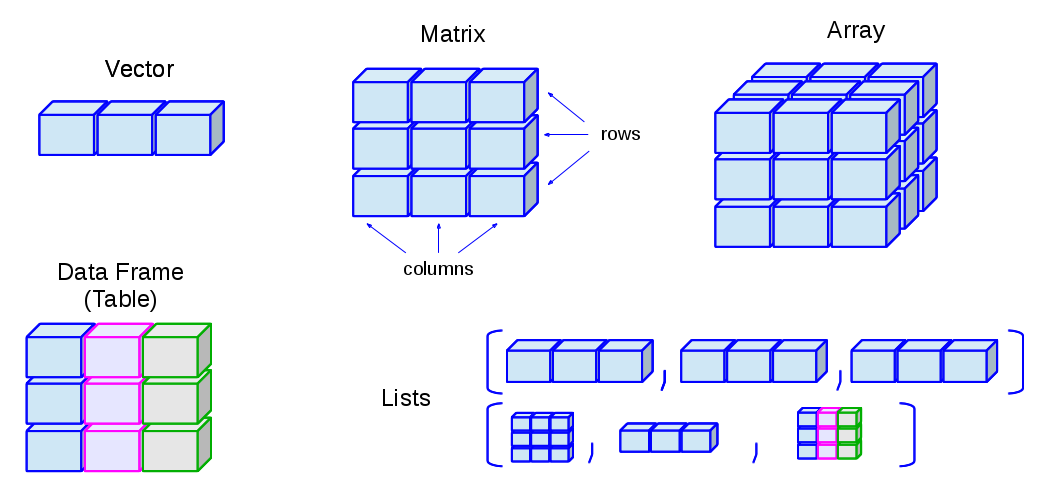
\includegraphics{./images/dataStructure.png}
\caption{}
\end{figure}

We have already seen data frames, vectors and factors. Let us have a
look to matrices, array and lists.

\subsection{Matrices}\label{matrices}

Matrices are generalizations of vectors. Like vectors, matrices need to
contain elements of the same kind.

\begin{Shaded}
\begin{Highlighting}[]
\KeywordTok{matrix}\NormalTok{(}\DecValTok{1}\NormalTok{:}\DecValTok{8}\NormalTok{, }\DataTypeTok{nrow =} \DecValTok{2}\NormalTok{, }\DataTypeTok{ncol =} \DecValTok{4}\NormalTok{)}
\end{Highlighting}
\end{Shaded}

\begin{verbatim}
##      [,1] [,2] [,3] [,4]
## [1,]    1    3    5    7
## [2,]    2    4    6    8
\end{verbatim}

\subsection{Array}\label{array}

They are similar to matrices but they can be multi-dimensional (more
than two dimensions)

\begin{Shaded}
\begin{Highlighting}[]
\NormalTok{z <-}\StringTok{ }\KeywordTok{array}\NormalTok{(}\DecValTok{1}\NormalTok{:}\DecValTok{24}\NormalTok{, }\DataTypeTok{dim=}\KeywordTok{c}\NormalTok{(}\DecValTok{2}\NormalTok{,}\DecValTok{3}\NormalTok{,}\DecValTok{4}\NormalTok{))}
\NormalTok{z}
\end{Highlighting}
\end{Shaded}

\begin{verbatim}
## , , 1
## 
##      [,1] [,2] [,3]
## [1,]    1    3    5
## [2,]    2    4    6
## 
## , , 2
## 
##      [,1] [,2] [,3]
## [1,]    7    9   11
## [2,]    8   10   12
## 
## , , 3
## 
##      [,1] [,2] [,3]
## [1,]   13   15   17
## [2,]   14   16   18
## 
## , , 4
## 
##      [,1] [,2] [,3]
## [1,]   19   21   23
## [2,]   20   22   24
\end{verbatim}

\subsection{Lists}\label{lists}

A list is an ordered collection of objects. Each object is a component
of the list. Each element of the list can have a different structure. It
can be a list itself, a vector, a matrix, an array, a factor or a data
frame. A list allows you to gather a variety of (possibly unrelated)
objects under one name.

\begin{Shaded}
\begin{Highlighting}[]
\NormalTok{my_list <-}\StringTok{ }\KeywordTok{list}\NormalTok{(}\DataTypeTok{vec =} \DecValTok{1}\NormalTok{:}\DecValTok{7}\NormalTok{, }\DataTypeTok{mat =} \KeywordTok{matrix}\NormalTok{(}\DecValTok{1}\NormalTok{:}\DecValTok{12}\NormalTok{, }\DataTypeTok{ncol =} \DecValTok{3}\NormalTok{),}
  \DataTypeTok{lis =} \KeywordTok{list}\NormalTok{(}\DataTypeTok{a =} \DecValTok{1}\NormalTok{, }\DataTypeTok{b =} \NormalTok{letters[}\DecValTok{1}\NormalTok{:}\DecValTok{4}\NormalTok{]))}
\NormalTok{my_list}
\end{Highlighting}
\end{Shaded}

\begin{verbatim}
## $vec
## [1] 1 2 3 4 5 6 7
## 
## $mat
##      [,1] [,2] [,3]
## [1,]    1    5    9
## [2,]    2    6   10
## [3,]    3    7   11
## [4,]    4    8   12
## 
## $lis
## $lis$a
## [1] 1
## 
## $lis$b
## [1] "a" "b" "c" "d"
\end{verbatim}

\chapter{Data Import from external
sources}\label{data-import-from-external-sources}

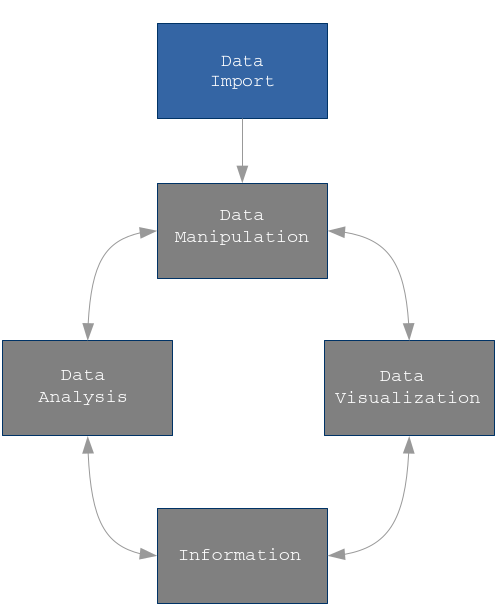
\includegraphics[width=3.33in]{images/flow-robj}

In the following paragraphs we will explore data import methods for:

\begin{itemize}
\tightlist
\item
  Text files
\item
  Microsoft Excel files
\item
  Databases
\end{itemize}

\section{Text files}\label{text-files}


\includegraphics[width=5.39in]{images/import-text}

The \texttt{read.table()} function imports a text file (ASCII) with a
table structure where each row represents a case.

A full path can be provided, but it must be modified by each user,
otherwise it fails:

\begin{Shaded}
\begin{Highlighting}[]
\NormalTok{df <-}\StringTok{ }\KeywordTok{read.table}\NormalTok{(}\StringTok{"C:/Users/UserName/Documents/data/tennis.txt"}\NormalTok{, }\DataTypeTok{header =} \OtherTok{TRUE}\NormalTok{, }\DataTypeTok{sep =} \StringTok{""}\NormalTok{, }\DataTypeTok{dec =} \StringTok{"."}\NormalTok{)}
\end{Highlighting}
\end{Shaded}

\begin{verbatim}
## Warning in file(file, "rt"): cannot open file 'C:/Users/UserName/Documents/
## data/tennis.txt': No such file or directory
\end{verbatim}

\begin{verbatim}
## Error in file(file, "rt"): cannot open the connection
\end{verbatim}

The path uses the slash (``\texttt{/}'') as delimiting character, in the
UNIX-like style. Under Windows, can be used both a slash character or a
doubled backslash character
(``\texttt{\textbackslash{}\textbackslash{}}'').

So, it is strongly suggested to set the working directory to the
directory containing the data.

\texttt{getwd()} function allows you to view the current working
directory:

\begin{Shaded}
\begin{Highlighting}[]
\KeywordTok{getwd}\NormalTok{() }
\end{Highlighting}
\end{Shaded}

\begin{verbatim}
## [1] "C:/Users/Andrea/Documents"
\end{verbatim}

and \texttt{setwd()} function allows you to set the working directory on
``data'' folder, in this way:

\begin{Shaded}
\begin{Highlighting}[]
\KeywordTok{setwd}\NormalTok{(}\StringTok{"./data"}\NormalTok{) }
\end{Highlighting}
\end{Shaded}

\begin{verbatim}
## [1] "C:/Users/Andrea/Documents/data"
\end{verbatim}

Now, the text file can be imported just providing its filename:

\begin{Shaded}
\begin{Highlighting}[]
\NormalTok{df <-}\StringTok{ }\KeywordTok{read.table}\NormalTok{(}\StringTok{"tennis.txt"}\NormalTok{, }\DataTypeTok{header =} \OtherTok{TRUE}\NormalTok{)}
\end{Highlighting}
\end{Shaded}

\begin{Shaded}
\begin{Highlighting}[]
\KeywordTok{head}\NormalTok{(df)}
\end{Highlighting}
\end{Shaded}

\begin{verbatim}
##         Name First.Name Age Sex Rank Slams Won Lost Earnings Citizen
## 1    Sampras       Pete  23   M    1     2  74   11 3607.812      US
## 2     Agassi      Andre  24   M    2     1  51   13 1941.667      US
## 3     Becker      Boris  27   M    3     0  48   16 2029.756 Germany
## 4   Bruguera      Sergi  24   M    4     1  65   23 3031.874   Spain
## 5 Ivanisevic      Goran  23   M    5     0  63   26 2060.278 Croatia
## 6       Graf     Steffi  25   F    1     1  58    6 1487.980 Germany
\end{verbatim}

\begin{Shaded}
\begin{Highlighting}[]
\KeywordTok{str}\NormalTok{(df)}
\end{Highlighting}
\end{Shaded}

\begin{verbatim}
## 'data.frame':    10 obs. of  10 variables:
##  $ Name      : Factor w/ 10 levels "Agassi","Becker",..: 9 1 2 3 5 4 10 6 7 8
##  $ First.Name: Factor w/ 10 levels "Andre","Arantxa",..: 8 1 3 9 5 10 2 4 6 7
##  $ Age       : int  23 24 27 24 23 25 23 22 26 20
##  $ Sex       : Factor w/ 2 levels "F","M": 2 2 2 2 2 1 1 1 1 1
##  $ Rank      : int  1 2 3 4 5 1 2 3 4 5
##  $ Slams     : int  2 1 0 1 0 1 2 1 0 0
##  $ Won       : int  74 51 48 65 63 58 74 55 43 45
##  $ Lost      : int  11 13 16 23 26 6 9 15 11 18
##  $ Earnings  : num  3608 1942 2030 3032 2060 ...
##  $ Citizen   : Factor w/ 6 levels "Croatia","Czech Republic",..: 6 6 4 5 1 4 5 5 2 3
\end{verbatim}

The \texttt{header\ =\ TRUE} option tells R that the first row of the
file contains column headings and it is used to assign the name of
variables. If the first row contains the first case the
\texttt{header\ =\ FALSE} ought to be used and the names of the
variables are automatically assigned.

The \texttt{sep} argument specifies the separator between different
cases. The default value for the \texttt{read.table()} function is
\texttt{sep\ =\ ""} which takes into consideration the fields delimited
by a white space, be it one or more spaces or tabulations.

The \texttt{dec} argument specifies the decimal separator. The argument
usually assumes the \texttt{dec\ =\ "."} (default) or
\texttt{dec\ =\ ","} values.

\begin{Shaded}
\begin{Highlighting}[]
\NormalTok{df <-}\StringTok{ }\KeywordTok{read.table}\NormalTok{(}\StringTok{"tennis.txt"}\NormalTok{, }\DataTypeTok{header =} \OtherTok{TRUE}\NormalTok{, }\DataTypeTok{sep =} \StringTok{""}\NormalTok{, }\DataTypeTok{dec =} \StringTok{"."}\NormalTok{)}
\KeywordTok{head}\NormalTok{(df)}
\end{Highlighting}
\end{Shaded}

\begin{verbatim}
##         Name First.Name Age Sex Rank Slams Won Lost Earnings Citizen
## 1    Sampras       Pete  23   M    1     2  74   11 3607.812      US
## 2     Agassi      Andre  24   M    2     1  51   13 1941.667      US
## 3     Becker      Boris  27   M    3     0  48   16 2029.756 Germany
## 4   Bruguera      Sergi  24   M    4     1  65   23 3031.874   Spain
## 5 Ivanisevic      Goran  23   M    5     0  63   26 2060.278 Croatia
## 6       Graf     Steffi  25   F    1     1  58    6 1487.980 Germany
\end{verbatim}

Variables containing text are set as character variables with the
\texttt{stringsAsFactors\ =\ FALSE} option, whereas by default they are
set as factors.

\begin{Shaded}
\begin{Highlighting}[]
\NormalTok{df <-}\StringTok{ }\KeywordTok{read.table}\NormalTok{(}\StringTok{"tennis.txt"}\NormalTok{, }\DataTypeTok{header =} \OtherTok{TRUE}\NormalTok{, }\DataTypeTok{sep =} \StringTok{""}\NormalTok{, }\DataTypeTok{dec =} \StringTok{"."}\NormalTok{, }\DataTypeTok{stringsAsFactors =} \OtherTok{FALSE}\NormalTok{)}
\KeywordTok{str}\NormalTok{(df)}
\end{Highlighting}
\end{Shaded}

\begin{verbatim}
## 'data.frame':    10 obs. of  10 variables:
##  $ Name      : chr  "Sampras" "Agassi" "Becker" "Bruguera" ...
##  $ First.Name: chr  "Pete" "Andre" "Boris" "Sergi" ...
##  $ Age       : int  23 24 27 24 23 25 23 22 26 20
##  $ Sex       : chr  "M" "M" "M" "M" ...
##  $ Rank      : int  1 2 3 4 5 1 2 3 4 5
##  $ Slams     : int  2 1 0 1 0 1 2 1 0 0
##  $ Won       : int  74 51 48 65 63 58 74 55 43 45
##  $ Lost      : int  11 13 16 23 26 6 9 15 11 18
##  $ Earnings  : num  3608 1942 2030 3032 2060 ...
##  $ Citizen   : chr  "US" "US" "Germany" "Spain" ...
\end{verbatim}

\section{Microsoft Excel files}\label{microsoft-excel-files}


\includegraphics[width=5.49in]{images/import-excel}

One of the most important R package for importing excel files into R is
\texttt{readxl}. Let us see how it works.

\begin{Shaded}
\begin{Highlighting}[]
\KeywordTok{require}\NormalTok{(readxl)}
\end{Highlighting}
\end{Shaded}

To read an existing excel file, the syntax is:

\begin{Shaded}
\begin{Highlighting}[]
\CommentTok{# Excel file (with path) to be loaded into R}
\NormalTok{file_xls <-}\StringTok{ "./xlsx/newFile.xlsx"}
\end{Highlighting}
\end{Shaded}

\begin{Shaded}
\begin{Highlighting}[]
\NormalTok{ds <-}\KeywordTok{read_excel}\NormalTok{(}\DataTypeTok{path =} \NormalTok{file_xls, }\DataTypeTok{sheet =} \StringTok{'Airquality'}\NormalTok{, }\DataTypeTok{col_names =} \OtherTok{TRUE}\NormalTok{)}
\KeywordTok{head}\NormalTok{(ds)}
\end{Highlighting}
\end{Shaded}

\begin{verbatim}
## # A tibble: 6 × 7
##   Ozone Solar.R  Wind  Temp Month   Day isCurrent
##   <dbl>   <dbl> <dbl> <dbl> <dbl> <dbl>     <dbl>
## 1    41     190   7.4    67     5     1         0
## 2    36     118   8.0    72     5     2         0
## 3    12     149  12.6    74     5     3         0
## 4    18     313  11.5    62     5     4         0
## 5    NA      NA  14.3    56     5     5         0
## 6    28      NA  14.9    66     5     6         0
\end{verbatim}

\texttt{read\_excel()} function allows us to read xls and xlsx files,
specified in \texttt{path} argument. \texttt{sheet} argument specifies
the sheet to read and \texttt{col\_names} indicates if the first row has
to be used as column names (set as \texttt{TRUE}).

\clearpage

\section{Databases}\label{databases}


\includegraphics[width=5.52in]{images/import-db}

\section{ODBC}\label{odbc}

Open Database Connectivity (ODBC) is a standard programming language
interface for accessing database management systems (DBMS). ODBC is
independent from database systems and operating systems. An application
can use ODBC to query data from a DBMS, regardless of the operating
system or DBMS it uses. ODBC accomplishes DBMS independence by using an
ODBC driver as a translation layer between the application and the DBMS.

With the \texttt{RODBC} package R enables the use of ODBC for
interacting with databases. This solution is particularly useful when
data occupies much space, is frequently updated or shared by two or more
users. In this case, data is kept in the database. With R it is possible
to make a query in the database, load data in the R workspace and carry
out analyses.

The following code shows some examples of how to use ODBC in a MySQL
database. For the following examples to work, it is necessary to modify
the following functions with the parameters related to the available
MySQL database.

The \texttt{odbcConnect()} function establishes the connection to the
MySQL database. Its main arguments are: \texttt{dsn}, a string
containing the name of the data source, \texttt{uid} and \texttt{pwd},
i.e.~the user name and the password for the login.\\
The \texttt{sqlQuery()} function performs queries to the MySQL database.
The use of single and double quotation marks require attention. In the
following example the query is contained in a string and is delimited by
double quotation marks. The strings belonging to the query are delimited
by single quotation marks.

Finally, the \texttt{odbcClose()} function closes the connection to the
database.

\begin{Shaded}
\begin{Highlighting}[]
\CommentTok{# RODBC driver ought be configured to work properly}
\KeywordTok{require}\NormalTok{(RODBC)}
\NormalTok{conn <-}\StringTok{ }\KeywordTok{odbcConnect}\NormalTok{(}\DataTypeTok{dsn =} \StringTok{"test"}\NormalTok{, }\DataTypeTok{uid =} \StringTok{"user"}\NormalTok{, }\DataTypeTok{pwd =} \StringTok{"pass"}\NormalTok{)}
\KeywordTok{sqlQuery}\NormalTok{(conn, }\StringTok{"select * from tbl where gender = 'F'"}\NormalTok{) }
\KeywordTok{odbcClose}\NormalTok{(conn)}
\end{Highlighting}
\end{Shaded}

\section{SQLlite}\label{sqllite}

\texttt{RSQLite} package embeds the SQLite database engine in R,
providing a DBI-compliant interface. SQLite is a public-domain,
single-user, very light-weight database engine that implements a decent
subset of the SQL 92 standard, including the core table creation,
updating, insertion, and selection operations, plus transaction
management.

\begin{Shaded}
\begin{Highlighting}[]
\KeywordTok{require}\NormalTok{(RSQLite)}
\end{Highlighting}
\end{Shaded}

The function \texttt{dbConnect} connect to a SQLite database, or creates
it if it doesn't exist:

\begin{Shaded}
\begin{Highlighting}[]
\NormalTok{con <-}\StringTok{ }\KeywordTok{dbConnect}\NormalTok{(RSQLite::}\KeywordTok{SQLite}\NormalTok{(), }\StringTok{"mtcars.sqlite"}\NormalTok{)}
\end{Highlighting}
\end{Shaded}

To see a list of available SQLite tables:

\begin{Shaded}
\begin{Highlighting}[]
\KeywordTok{dbListTables}\NormalTok{(con)}
\end{Highlighting}
\end{Shaded}

\begin{verbatim}
## [1] "mtcars"
\end{verbatim}

or a list of fields in specified table:

\begin{Shaded}
\begin{Highlighting}[]
\KeywordTok{dbListFields}\NormalTok{(con, }\StringTok{"mtcars"}\NormalTok{)}
\end{Highlighting}
\end{Shaded}

\begin{verbatim}
##  [1] "row_names" "mpg"       "cyl"       "disp"      "hp"       
##  [6] "drat"      "wt"        "qsec"      "vs"        "am"       
## [11] "gear"      "carb"
\end{verbatim}

The next function mimic its R/S-Plus counterpart \texttt{get}, except
that it generates code that gets remotely executed in a database engine:

\begin{Shaded}
\begin{Highlighting}[]
\KeywordTok{dbReadTable}\NormalTok{(con, }\StringTok{"mtcars"}\NormalTok{)}
\end{Highlighting}
\end{Shaded}

\begin{verbatim}
##                      mpg cyl  disp  hp drat    wt  qsec vs am gear carb
## Mazda RX4           21.0   6 160.0 110 3.90 2.620 16.46  0  1    4    4
## Mazda RX4 Wag       21.0   6 160.0 110 3.90 2.875 17.02  0  1    4    4
## Datsun 710          22.8   4 108.0  93 3.85 2.320 18.61  1  1    4    1
## Hornet 4 Drive      21.4   6 258.0 110 3.08 3.215 19.44  1  0    3    1
## Hornet Sportabout   18.7   8 360.0 175 3.15 3.440 17.02  0  0    3    2
## Valiant             18.1   6 225.0 105 2.76 3.460 20.22  1  0    3    1
## Duster 360          14.3   8 360.0 245 3.21 3.570 15.84  0  0    3    4
## Merc 240D           24.4   4 146.7  62 3.69 3.190 20.00  1  0    4    2
## Merc 230            22.8   4 140.8  95 3.92 3.150 22.90  1  0    4    2
## Merc 280            19.2   6 167.6 123 3.92 3.440 18.30  1  0    4    4
## Merc 280C           17.8   6 167.6 123 3.92 3.440 18.90  1  0    4    4
## Merc 450SE          16.4   8 275.8 180 3.07 4.070 17.40  0  0    3    3
## Merc 450SL          17.3   8 275.8 180 3.07 3.730 17.60  0  0    3    3
## Merc 450SLC         15.2   8 275.8 180 3.07 3.780 18.00  0  0    3    3
## Cadillac Fleetwood  10.4   8 472.0 205 2.93 5.250 17.98  0  0    3    4
## Lincoln Continental 10.4   8 460.0 215 3.00 5.424 17.82  0  0    3    4
## Chrysler Imperial   14.7   8 440.0 230 3.23 5.345 17.42  0  0    3    4
## Fiat 128            32.4   4  78.7  66 4.08 2.200 19.47  1  1    4    1
## Honda Civic         30.4   4  75.7  52 4.93 1.615 18.52  1  1    4    2
## Toyota Corolla      33.9   4  71.1  65 4.22 1.835 19.90  1  1    4    1
## Toyota Corona       21.5   4 120.1  97 3.70 2.465 20.01  1  0    3    1
## Dodge Challenger    15.5   8 318.0 150 2.76 3.520 16.87  0  0    3    2
## AMC Javelin         15.2   8 304.0 150 3.15 3.435 17.30  0  0    3    2
## Camaro Z28          13.3   8 350.0 245 3.73 3.840 15.41  0  0    3    4
## Pontiac Firebird    19.2   8 400.0 175 3.08 3.845 17.05  0  0    3    2
## Fiat X1-9           27.3   4  79.0  66 4.08 1.935 18.90  1  1    4    1
## Porsche 914-2       26.0   4 120.3  91 4.43 2.140 16.70  0  1    5    2
## Lotus Europa        30.4   4  95.1 113 3.77 1.513 16.90  1  1    5    2
## Ford Pantera L      15.8   8 351.0 264 4.22 3.170 14.50  0  1    5    4
## Ferrari Dino        19.7   6 145.0 175 3.62 2.770 15.50  0  1    5    6
## Maserati Bora       15.0   8 301.0 335 3.54 3.570 14.60  0  1    5    8
## Volvo 142E          21.4   4 121.0 109 4.11 2.780 18.60  1  1    4    2
\end{verbatim}

The function \texttt{dbGetQuery} send query, retrieve results and then
clear result set:

\begin{Shaded}
\begin{Highlighting}[]
\KeywordTok{dbGetQuery}\NormalTok{(con, }\StringTok{"SELECT * FROM mtcars WHERE cyl = 4"}\NormalTok{)}
\end{Highlighting}
\end{Shaded}

\begin{verbatim}
##         row_names  mpg cyl  disp  hp drat    wt  qsec vs am gear carb
## 1      Datsun 710 22.8   4 108.0  93 3.85 2.320 18.61  1  1    4    1
## 2       Merc 240D 24.4   4 146.7  62 3.69 3.190 20.00  1  0    4    2
## 3        Merc 230 22.8   4 140.8  95 3.92 3.150 22.90  1  0    4    2
## 4        Fiat 128 32.4   4  78.7  66 4.08 2.200 19.47  1  1    4    1
## 5     Honda Civic 30.4   4  75.7  52 4.93 1.615 18.52  1  1    4    2
## 6  Toyota Corolla 33.9   4  71.1  65 4.22 1.835 19.90  1  1    4    1
## 7   Toyota Corona 21.5   4 120.1  97 3.70 2.465 20.01  1  0    3    1
## 8       Fiat X1-9 27.3   4  79.0  66 4.08 1.935 18.90  1  1    4    1
## 9   Porsche 914-2 26.0   4 120.3  91 4.43 2.140 16.70  0  1    5    2
## 10   Lotus Europa 30.4   4  95.1 113 3.77 1.513 16.90  1  1    5    2
## 11     Volvo 142E 21.4   4 121.0 109 4.11 2.780 18.60  1  1    4    2
\end{verbatim}

And finally disconnect from the database:

\begin{Shaded}
\begin{Highlighting}[]
\KeywordTok{dbDisconnect}\NormalTok{(con)}
\end{Highlighting}
\end{Shaded}

\begin{verbatim}
## [1] TRUE
\end{verbatim}

\chapter{Data Manipulation with R}\label{data-manipulation-with-r}

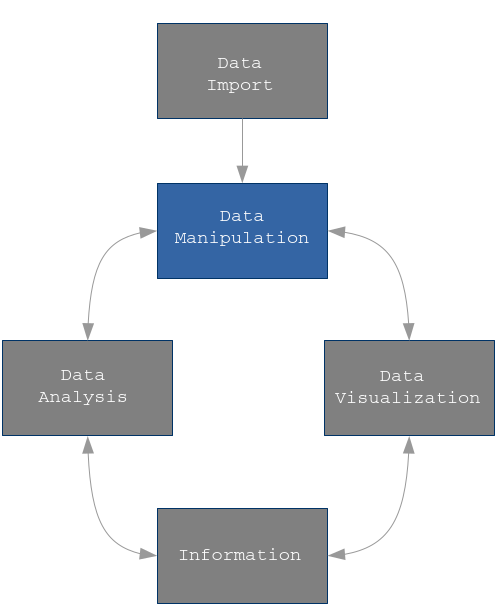
\includegraphics[width=3.33in]{images/flow-dtman}

The \texttt{dplyr} package for \texttt{R} is very powerful for data
management since:

\begin{itemize}
\tightlist
\item
  it simplifies how you can think about common data manipulation tasks
\item
  it provides simple ``verbs'', functions that correspond to the most
  common data manipulation tasks
\item
  it uses efficient data storage backends, so you spend less time
  waiting for the computer
\end{itemize}

\begin{Shaded}
\begin{Highlighting}[]
\KeywordTok{require}\NormalTok{(dplyr)}
\end{Highlighting}
\end{Shaded}

The examples of this chapter will refer to \texttt{bank} data set which
contains information about a direct marketing campaigns of a Portuguese
banking institution based on phone calls.

\begin{Shaded}
\begin{Highlighting}[]
\KeywordTok{require}\NormalTok{(qdata)}
\KeywordTok{data}\NormalTok{(bank) }
\NormalTok{bank}
\end{Highlighting}
\end{Shaded}

\begin{verbatim}
## # A tibble: 45,211 × 20
##       id   age          job  marital education default balance housing
##    <int> <int>       <fctr>   <fctr>    <fctr>  <fctr>   <int>  <fctr>
## 1      1    58   management  married  tertiary      no    2143     yes
## 2      2    44   technician   single secondary      no      29     yes
## 3      3    33 entrepreneur  married secondary      no       2     yes
## 4      4    47  blue-collar  married   unknown      no    1506     yes
## 5      5    33      unknown   single   unknown      no       1      no
## 6      6    35   management  married  tertiary      no     231     yes
## 7      7    28   management   single  tertiary      no     447     yes
## 8      8    42 entrepreneur divorced  tertiary     yes       2     yes
## 9      9    58      retired  married   primary      no     121     yes
## 10    10    43   technician   single secondary      no     593     yes
## # ... with 45,201 more rows, and 12 more variables: loan <fctr>,
## #   contact <fctr>, day <int>, month <fctr>, year <int>, date <dttm>,
## #   duration <int>, campaign <int>, pdays <int>, previous <int>,
## #   poutcome <fctr>, y <fctr>
\end{verbatim}

In the following paragraphs, we will explore the innovations introduced
by \texttt{dplyr} to make our lifes easier when dealing with dataframes
manipulation tasks.\\
In particular:

\begin{itemize}
\tightlist
\item
  pipe operator (\texttt{\%\textgreater{}\%})
\item
  dplyr verbs for data manipulation
\item
  dplyr verbs for combining data
\end{itemize}

\section{\texorpdfstring{Pipe operator
(\texttt{\%\textgreater{}\%})}{Pipe operator (\%\textgreater{}\%)}}\label{pipe-operator}

\texttt{dplyr} pipe operator (\texttt{\%\textgreater{}\%}) allows us to
pipe the output from one function to the input of another function. The
idea of piping is to read the functions from left to right. It is
particularly useful with nested functions (reading from the inside to
the outside) or with multiple operations.

\clearpage

\begin{figure}
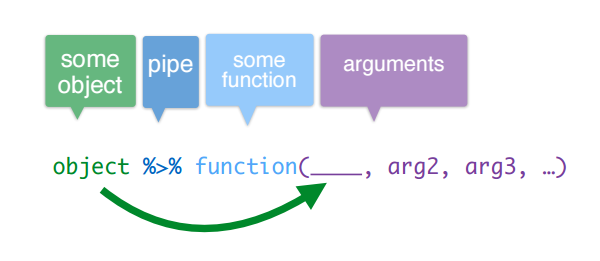
\includegraphics[width=4in]{images/pipe} \caption{Source: www.datacamp.com}\label{fig:g2}
\end{figure}

Pipes can work with nearly any functions (\texttt{dplyr} and
not-\texttt{dplyr} functions), let us see an example.

Suppose we want to visualize the first rows of \texttt{bank} dataframe,
by using \texttt{head()} function.

Usually we write:

\begin{Shaded}
\begin{Highlighting}[]
\KeywordTok{head}\NormalTok{(bank)}
\end{Highlighting}
\end{Shaded}

\begin{verbatim}
## # A tibble: 6 × 20
##      id   age          job marital education default balance housing
##   <int> <int>       <fctr>  <fctr>    <fctr>  <fctr>   <int>  <fctr>
## 1     1    58   management married  tertiary      no    2143     yes
## 2     2    44   technician  single secondary      no      29     yes
## 3     3    33 entrepreneur married secondary      no       2     yes
## 4     4    47  blue-collar married   unknown      no    1506     yes
## 5     5    33      unknown  single   unknown      no       1      no
## 6     6    35   management married  tertiary      no     231     yes
## # ... with 12 more variables: loan <fctr>, contact <fctr>, day <int>,
## #   month <fctr>, year <int>, date <dttm>, duration <int>, campaign <int>,
## #   pdays <int>, previous <int>, poutcome <fctr>, y <fctr>
\end{verbatim}

By using \texttt{\%\textgreater{}\%}, the code becomes:

\begin{Shaded}
\begin{Highlighting}[]
\NormalTok{bank %>%}\StringTok{ }\KeywordTok{head}\NormalTok{()}
\end{Highlighting}
\end{Shaded}

\begin{verbatim}
## # A tibble: 6 × 20
##      id   age          job marital education default balance housing
##   <int> <int>       <fctr>  <fctr>    <fctr>  <fctr>   <int>  <fctr>
## 1     1    58   management married  tertiary      no    2143     yes
## 2     2    44   technician  single secondary      no      29     yes
## 3     3    33 entrepreneur married secondary      no       2     yes
## 4     4    47  blue-collar married   unknown      no    1506     yes
## 5     5    33      unknown  single   unknown      no       1      no
## 6     6    35   management married  tertiary      no     231     yes
## # ... with 12 more variables: loan <fctr>, contact <fctr>, day <int>,
## #   month <fctr>, year <int>, date <dttm>, duration <int>, campaign <int>,
## #   pdays <int>, previous <int>, poutcome <fctr>, y <fctr>
\end{verbatim}

Pipe takes the argument on the left (\texttt{bank}) and passes it to the
function on the right (\texttt{head()}). So you don't need to write the
first argument of the function.

Other arguments of the function must be added to the function itself, as
usually done. By default \texttt{head()} prints the first 6 rows of the
dataframe. Suppose we want to print 10 rows, by setting \texttt{n}
argument to 10:

\begin{Shaded}
\begin{Highlighting}[]
\NormalTok{bank %>%}\StringTok{ }\KeywordTok{head}\NormalTok{(}\DataTypeTok{n=}\DecValTok{10}\NormalTok{)}
\end{Highlighting}
\end{Shaded}

\begin{verbatim}
## # A tibble: 10 × 20
##       id   age          job  marital education default balance housing
##    <int> <int>       <fctr>   <fctr>    <fctr>  <fctr>   <int>  <fctr>
## 1      1    58   management  married  tertiary      no    2143     yes
## 2      2    44   technician   single secondary      no      29     yes
## 3      3    33 entrepreneur  married secondary      no       2     yes
## 4      4    47  blue-collar  married   unknown      no    1506     yes
## 5      5    33      unknown   single   unknown      no       1      no
## 6      6    35   management  married  tertiary      no     231     yes
## 7      7    28   management   single  tertiary      no     447     yes
## 8      8    42 entrepreneur divorced  tertiary     yes       2     yes
## 9      9    58      retired  married   primary      no     121     yes
## 10    10    43   technician   single secondary      no     593     yes
## # ... with 12 more variables: loan <fctr>, contact <fctr>, day <int>,
## #   month <fctr>, year <int>, date <dttm>, duration <int>, campaign <int>,
## #   pdays <int>, previous <int>, poutcome <fctr>, y <fctr>
\end{verbatim}

\clearpage

\section{dplyr verbs for data
manipulation}\label{dplyr-verbs-for-data-manipulation}

\texttt{dplyr} aims to provide a function for each basic verb of data
manipulation and data discovery.

All these functions are very similar:

\begin{itemize}
\tightlist
\item
  the first argument is a data frame;
\item
  the subsequent arguments describe what to do with it, and you can
  refer to columns in the data frame directly without using \$. Note
  that the column names must be unquoted;
\item
  the result is a new data frame.
\end{itemize}

Let us have a look to \texttt{dplyr} verbs for data manipulation:

\begin{itemize}
\tightlist
\item
  \texttt{select()}: select variables of interest
\item
  \texttt{filter()}: filter records of interest
\item
  \texttt{arrange()}: reorder the rows
\item
  \texttt{mutate()}: add new variables that are functions of existing
  ones
\end{itemize}

\subsection{\texorpdfstring{\texttt{select()}}{select()}}\label{select}

Often you work with large datasets with many columns where only a few
are actually of interest to you.

\texttt{select()} allows you to rapidly zoom in on a useful subset of
columns.

\begin{figure}[htbp]
\centering
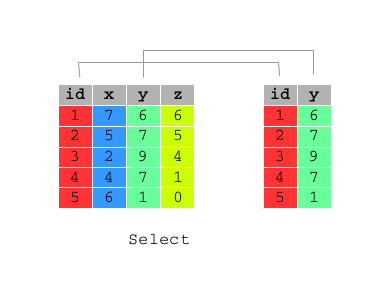
\includegraphics{images/sel.png}
\caption{}
\end{figure}

\begin{Shaded}
\begin{Highlighting}[]
\CommentTok{# Select columns: year, month and day of bank data frame}
\KeywordTok{select}\NormalTok{(bank, year, month, day)}
\end{Highlighting}
\end{Shaded}

\begin{verbatim}
## # A tibble: 45,211 × 3
##     year  month   day
##    <int> <fctr> <int>
## 1   2008    may     5
## 2   2008    may     5
## 3   2008    may     5
## 4   2008    may     5
## 5   2008    may     5
## 6   2008    may     5
## 7   2008    may     5
## 8   2008    may     5
## 9   2008    may     5
## 10  2008    may     5
## # ... with 45,201 more rows
\end{verbatim}

\begin{Shaded}
\begin{Highlighting}[]
\CommentTok{# Select columns: year, month and day of bank data frame}
\NormalTok{bank %>%}\StringTok{ }\KeywordTok{select}\NormalTok{(year:day)}
\end{Highlighting}
\end{Shaded}

\begin{verbatim}
## # A tibble: 45,211 × 3
##     year  month   day
##    <int> <fctr> <int>
## 1   2008    may     5
## 2   2008    may     5
## 3   2008    may     5
## 4   2008    may     5
## 5   2008    may     5
## 6   2008    may     5
## 7   2008    may     5
## 8   2008    may     5
## 9   2008    may     5
## 10  2008    may     5
## # ... with 45,201 more rows
\end{verbatim}

\begin{Shaded}
\begin{Highlighting}[]
\CommentTok{# Select all columns of bank data frame apart from: year, month and day}
\NormalTok{bank %>%}\StringTok{ }\KeywordTok{select}\NormalTok{(-(year:day))}
\end{Highlighting}
\end{Shaded}

\begin{verbatim}
## # A tibble: 45,211 × 17
##       id   age          job  marital education default balance housing
##    <int> <int>       <fctr>   <fctr>    <fctr>  <fctr>   <int>  <fctr>
## 1      1    58   management  married  tertiary      no    2143     yes
## 2      2    44   technician   single secondary      no      29     yes
## 3      3    33 entrepreneur  married secondary      no       2     yes
## 4      4    47  blue-collar  married   unknown      no    1506     yes
## 5      5    33      unknown   single   unknown      no       1      no
## 6      6    35   management  married  tertiary      no     231     yes
## 7      7    28   management   single  tertiary      no     447     yes
## 8      8    42 entrepreneur divorced  tertiary     yes       2     yes
## 9      9    58      retired  married   primary      no     121     yes
## 10    10    43   technician   single secondary      no     593     yes
## # ... with 45,201 more rows, and 9 more variables: loan <fctr>,
## #   contact <fctr>, date <dttm>, duration <int>, campaign <int>,
## #   pdays <int>, previous <int>, poutcome <fctr>, y <fctr>
\end{verbatim}

You can rename variables with \texttt{select()} by using named
arguments:

\begin{Shaded}
\begin{Highlighting}[]
\CommentTok{# Rename id variable as ID}
\NormalTok{bank %>%}\StringTok{ }\KeywordTok{select}\NormalTok{(}\DataTypeTok{ID =} \NormalTok{id)}
\end{Highlighting}
\end{Shaded}

\begin{verbatim}
## # A tibble: 45,211 × 1
##       ID
##    <int>
## 1      1
## 2      2
## 3      3
## 4      4
## 5      5
## 6      6
## 7      7
## 8      8
## 9      9
## 10    10
## # ... with 45,201 more rows
\end{verbatim}

\subsection{\texorpdfstring{\texttt{filter()}}{filter()}}\label{filter}

\texttt{filter()} allows you to select a subset of the rows of a data
frame.

\begin{figure}[htbp]
\centering
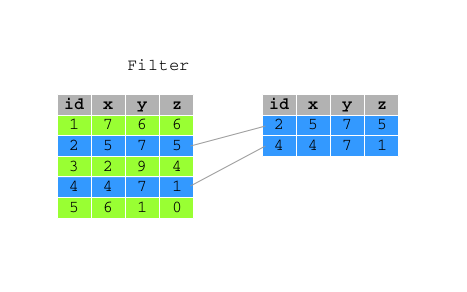
\includegraphics{images/fil.png}
\caption{}
\end{figure}

\begin{Shaded}
\begin{Highlighting}[]
\CommentTok{# filter all calls made to students with balance above 20,000 in bank data frame}
\KeywordTok{filter}\NormalTok{(bank, job ==}\StringTok{ "student"}\NormalTok{, balance >}\StringTok{ }\DecValTok{20000}\NormalTok{)}
\end{Highlighting}
\end{Shaded}

\begin{verbatim}
## # A tibble: 3 × 20
##      id   age     job marital education default balance housing   loan
##   <int> <int>  <fctr>  <fctr>    <fctr>  <fctr>   <int>  <fctr> <fctr>
## 1 31125    24 student  single secondary      no   23878      no     no
## 2 39536    24 student  single secondary      no   23878      no     no
## 3 41923    27 student  single  tertiary      no   24025      no     no
## # ... with 11 more variables: contact <fctr>, day <int>, month <fctr>,
## #   year <int>, date <dttm>, duration <int>, campaign <int>, pdays <int>,
## #   previous <int>, poutcome <fctr>, y <fctr>
\end{verbatim}

\texttt{filter()} allows you to give it any number of filtering
conditions which are joined together with \texttt{\&} and/or the other
operators.

\begin{Shaded}
\begin{Highlighting}[]
\CommentTok{# Filter all calls made to student of 18 years in bank data frame}
\NormalTok{bank %>%}\StringTok{ }\KeywordTok{filter}\NormalTok{(age ==}\StringTok{ }\DecValTok{18} \NormalTok{&}\StringTok{ }\NormalTok{job ==}\StringTok{ "student"}\NormalTok{)}
\end{Highlighting}
\end{Shaded}

\begin{verbatim}
## # A tibble: 12 × 20
##       id   age     job marital education default balance housing   loan
##    <int> <int>  <fctr>  <fctr>    <fctr>  <fctr>   <int>  <fctr> <fctr>
## 1  40737    18 student  single   primary      no    1944      no     no
## 2  40745    18 student  single   unknown      no     108      no     no
## 3  40888    18 student  single   primary      no     608      no     no
## 4  41223    18 student  single   unknown      no      35      no     no
## 5  41253    18 student  single secondary      no       5      no     no
## 6  41274    18 student  single   unknown      no       3      no     no
## 7  41488    18 student  single   unknown      no     108      no     no
## 8  42147    18 student  single secondary      no     156      no     no
## 9  42275    18 student  single   primary      no     608      no     no
## 10 42955    18 student  single   unknown      no     108      no     no
## 11 43638    18 student  single   unknown      no     348      no     no
## 12 44645    18 student  single   unknown      no     438      no     no
## # ... with 11 more variables: contact <fctr>, day <int>, month <fctr>,
## #   year <int>, date <dttm>, duration <int>, campaign <int>, pdays <int>,
## #   previous <int>, poutcome <fctr>, y <fctr>
\end{verbatim}

\begin{Shaded}
\begin{Highlighting}[]
\CommentTok{# Filter all calls made to people of 18 or 95 years in bank data frame}
\NormalTok{bank %>%}\StringTok{ }\KeywordTok{filter}\NormalTok{(age ==}\StringTok{ }\DecValTok{18} \NormalTok{|}\StringTok{ }\NormalTok{age ==}\StringTok{ }\DecValTok{95}\NormalTok{)}
\end{Highlighting}
\end{Shaded}

\begin{verbatim}
## # A tibble: 14 × 20
##       id   age     job  marital education default balance housing   loan
##    <int> <int>  <fctr>   <fctr>    <fctr>  <fctr>   <int>  <fctr> <fctr>
## 1  33700    95 retired divorced   primary      no    2282      no     no
## 2  40737    18 student   single   primary      no    1944      no     no
## 3  40745    18 student   single   unknown      no     108      no     no
## 4  40888    18 student   single   primary      no     608      no     no
## 5  41223    18 student   single   unknown      no      35      no     no
## 6  41253    18 student   single secondary      no       5      no     no
## 7  41274    18 student   single   unknown      no       3      no     no
## 8  41488    18 student   single   unknown      no     108      no     no
## 9  41664    95 retired  married secondary      no       0      no     no
## 10 42147    18 student   single secondary      no     156      no     no
## 11 42275    18 student   single   primary      no     608      no     no
## 12 42955    18 student   single   unknown      no     108      no     no
## 13 43638    18 student   single   unknown      no     348      no     no
## 14 44645    18 student   single   unknown      no     438      no     no
## # ... with 11 more variables: contact <fctr>, day <int>, month <fctr>,
## #   year <int>, date <dttm>, duration <int>, campaign <int>, pdays <int>,
## #   previous <int>, poutcome <fctr>, y <fctr>
\end{verbatim}

\texttt{filter()} can be used also with \texttt{\%in\%} to establish
conditions under which filter:

\begin{Shaded}
\begin{Highlighting}[]
\CommentTok{# Filter all calls made to people of 18 or 95 years in bank data frame}
\NormalTok{bank %>%}\StringTok{ }\KeywordTok{filter}\NormalTok{(age %in%}\StringTok{ }\KeywordTok{c}\NormalTok{(}\DecValTok{18}\NormalTok{,}\DecValTok{95}\NormalTok{))}
\end{Highlighting}
\end{Shaded}

\begin{verbatim}
## # A tibble: 14 × 20
##       id   age     job  marital education default balance housing   loan
##    <int> <int>  <fctr>   <fctr>    <fctr>  <fctr>   <int>  <fctr> <fctr>
## 1  33700    95 retired divorced   primary      no    2282      no     no
## 2  40737    18 student   single   primary      no    1944      no     no
## 3  40745    18 student   single   unknown      no     108      no     no
## 4  40888    18 student   single   primary      no     608      no     no
## 5  41223    18 student   single   unknown      no      35      no     no
## 6  41253    18 student   single secondary      no       5      no     no
## 7  41274    18 student   single   unknown      no       3      no     no
## 8  41488    18 student   single   unknown      no     108      no     no
## 9  41664    95 retired  married secondary      no       0      no     no
## 10 42147    18 student   single secondary      no     156      no     no
## 11 42275    18 student   single   primary      no     608      no     no
## 12 42955    18 student   single   unknown      no     108      no     no
## 13 43638    18 student   single   unknown      no     348      no     no
## 14 44645    18 student   single   unknown      no     438      no     no
## # ... with 11 more variables: contact <fctr>, day <int>, month <fctr>,
## #   year <int>, date <dttm>, duration <int>, campaign <int>, pdays <int>,
## #   previous <int>, poutcome <fctr>, y <fctr>
\end{verbatim}

\begin{Shaded}
\begin{Highlighting}[]
\CommentTok{# Filter all calls made to people whose job is admin. or technician in bank data frame}
\NormalTok{bank %>%}\StringTok{ }\KeywordTok{filter}\NormalTok{(job %in%}\StringTok{ }\KeywordTok{c}\NormalTok{(}\StringTok{"admin."}\NormalTok{,}\StringTok{"technician"}\NormalTok{))}
\end{Highlighting}
\end{Shaded}

\begin{verbatim}
## # A tibble: 12,768 × 20
##       id   age        job  marital education default balance housing
##    <int> <int>     <fctr>   <fctr>    <fctr>  <fctr>   <int>  <fctr>
## 1      2    44 technician   single secondary      no      29     yes
## 2     10    43 technician   single secondary      no     593     yes
## 3     11    41     admin. divorced secondary      no     270     yes
## 4     12    29     admin.   single secondary      no     390     yes
## 5     13    53 technician  married secondary      no       6     yes
## 6     14    58 technician  married   unknown      no      71     yes
## 7     17    45     admin.   single   unknown      no      13     yes
## 8     26    44     admin.  married secondary      no    -372     yes
## 9     30    36 technician   single secondary      no     265     yes
## 10    31    57 technician  married secondary      no     839      no
## # ... with 12,758 more rows, and 12 more variables: loan <fctr>,
## #   contact <fctr>, day <int>, month <fctr>, year <int>, date <dttm>,
## #   duration <int>, campaign <int>, pdays <int>, previous <int>,
## #   poutcome <fctr>, y <fctr>
\end{verbatim}

\begin{Shaded}
\begin{Highlighting}[]
\CommentTok{# Filter all calls made to people whose job is admin. or technician in bank data frame}
\NormalTok{bank %>%}\StringTok{ }\KeywordTok{filter}\NormalTok{(job ==}\StringTok{ "admin."} \NormalTok{|}\StringTok{ }\NormalTok{job ==}\StringTok{ "technician"}\NormalTok{)}
\end{Highlighting}
\end{Shaded}

\begin{verbatim}
## # A tibble: 12,768 × 20
##       id   age        job  marital education default balance housing
##    <int> <int>     <fctr>   <fctr>    <fctr>  <fctr>   <int>  <fctr>
## 1      2    44 technician   single secondary      no      29     yes
## 2     10    43 technician   single secondary      no     593     yes
## 3     11    41     admin. divorced secondary      no     270     yes
## 4     12    29     admin.   single secondary      no     390     yes
## 5     13    53 technician  married secondary      no       6     yes
## 6     14    58 technician  married   unknown      no      71     yes
## 7     17    45     admin.   single   unknown      no      13     yes
## 8     26    44     admin.  married secondary      no    -372     yes
## 9     30    36 technician   single secondary      no     265     yes
## 10    31    57 technician  married secondary      no     839      no
## # ... with 12,758 more rows, and 12 more variables: loan <fctr>,
## #   contact <fctr>, day <int>, month <fctr>, year <int>, date <dttm>,
## #   duration <int>, campaign <int>, pdays <int>, previous <int>,
## #   poutcome <fctr>, y <fctr>
\end{verbatim}

\subsection{\texorpdfstring{\texttt{arrange()}}{arrange()}}\label{arrange}

Function \texttt{arrange()} reorders a data frame by one or more
variables. If you provide more than one column name, each additional
column will be used to break ties in the values of preceding columns:

\begin{figure}[htbp]
\centering
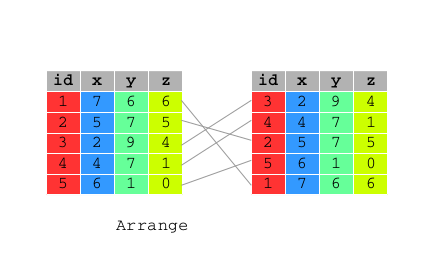
\includegraphics{images/arr.png}
\caption{}
\end{figure}

\begin{Shaded}
\begin{Highlighting}[]
\CommentTok{# Order `bank` data frame by the balance of the account in ascending order}
\KeywordTok{arrange}\NormalTok{(bank, balance)}
\end{Highlighting}
\end{Shaded}

\begin{verbatim}
## # A tibble: 45,211 × 20
##       id   age           job  marital education default balance housing
##    <int> <int>        <fctr>   <fctr>    <fctr>  <fctr>   <int>  <fctr>
## 1  12910    26   blue-collar   single secondary     yes   -8019      no
## 2  15683    49    management  married  tertiary     yes   -6847      no
## 3  38737    60    management divorced  tertiary      no   -4057     yes
## 4   7414    43    management  married  tertiary     yes   -3372     yes
## 5   1897    57 self-employed  married  tertiary     yes   -3313     yes
## 6  32714    39 self-employed  married  tertiary      no   -3058     yes
## 7  18574    40    technician  married  tertiary     yes   -2827     yes
## 8  31510    52    management  married  tertiary      no   -2712     yes
## 9  25120    49   blue-collar   single   primary     yes   -2604     yes
## 10 14435    51    management divorced  tertiary      no   -2282     yes
## # ... with 45,201 more rows, and 12 more variables: loan <fctr>,
## #   contact <fctr>, day <int>, month <fctr>, year <int>, date <dttm>,
## #   duration <int>, campaign <int>, pdays <int>, previous <int>,
## #   poutcome <fctr>, y <fctr>
\end{verbatim}

\begin{Shaded}
\begin{Highlighting}[]
\CommentTok{# Order `bank` data frame by the balance of the account in descending order}
\NormalTok{bank %>%}\StringTok{ }\KeywordTok{arrange}\NormalTok{(}\KeywordTok{desc}\NormalTok{(balance))}
\end{Highlighting}
\end{Shaded}

\begin{verbatim}
## # A tibble: 45,211 × 20
##       id   age          job  marital education default balance housing
##    <int> <int>       <fctr>   <fctr>    <fctr>  <fctr>   <int>  <fctr>
## 1  39990    51   management   single  tertiary      no  102127      no
## 2  26228    59   management  married  tertiary      no   98417      no
## 3  42559    84      retired  married secondary      no   81204      no
## 4  43394    84      retired  married secondary      no   81204      no
## 5  41694    60      retired  married   primary      no   71188      no
## 6  19786    56   management divorced  tertiary      no   66721      no
## 7  21193    52  blue-collar  married   primary      no   66653      no
## 8  19421    59       admin.  married   unknown      no   64343      no
## 9  41375    32 entrepreneur   single  tertiary      no   59649      no
## 10 12927    56  blue-collar  married secondary      no   58932      no
## # ... with 45,201 more rows, and 12 more variables: loan <fctr>,
## #   contact <fctr>, day <int>, month <fctr>, year <int>, date <dttm>,
## #   duration <int>, campaign <int>, pdays <int>, previous <int>,
## #   poutcome <fctr>, y <fctr>
\end{verbatim}

\begin{Shaded}
\begin{Highlighting}[]
\CommentTok{# Order `bank` data frame by age of the client and by the balance of the account in descending order}
\NormalTok{bank %>%}\StringTok{ }\KeywordTok{arrange}\NormalTok{(age, }\KeywordTok{desc}\NormalTok{(balance))}
\end{Highlighting}
\end{Shaded}

\begin{verbatim}
## # A tibble: 45,211 × 20
##       id   age     job marital education default balance housing   loan
##    <int> <int>  <fctr>  <fctr>    <fctr>  <fctr>   <int>  <fctr> <fctr>
## 1  40737    18 student  single   primary      no    1944      no     no
## 2  40888    18 student  single   primary      no     608      no     no
## 3  42275    18 student  single   primary      no     608      no     no
## 4  44645    18 student  single   unknown      no     438      no     no
## 5  43638    18 student  single   unknown      no     348      no     no
## 6  42147    18 student  single secondary      no     156      no     no
## 7  40745    18 student  single   unknown      no     108      no     no
## 8  41488    18 student  single   unknown      no     108      no     no
## 9  42955    18 student  single   unknown      no     108      no     no
## 10 41223    18 student  single   unknown      no      35      no     no
## # ... with 45,201 more rows, and 11 more variables: contact <fctr>,
## #   day <int>, month <fctr>, year <int>, date <dttm>, duration <int>,
## #   campaign <int>, pdays <int>, previous <int>, poutcome <fctr>, y <fctr>
\end{verbatim}

\clearpage

\subsection{\texorpdfstring{\texttt{mutate()}}{mutate()}}\label{mutate}

As well as selecting from the set of existing columns, it's often useful
to add new columns that are functions of existing ones. This is the job
of \texttt{mutate()}:

\begin{figure}[htbp]
\centering
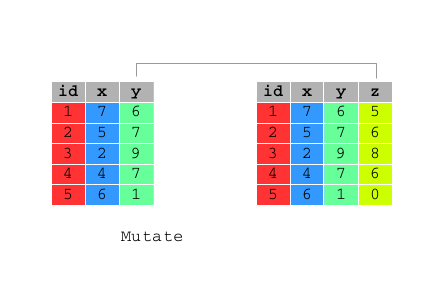
\includegraphics{images/mut.png}
\caption{}
\end{figure}

\begin{Shaded}
\begin{Highlighting}[]
\CommentTok{# generate a variable indicating the total number of times each person has been contacted }
\CommentTok{# during this campaign and during the previous ones }
\KeywordTok{mutate}\NormalTok{(bank, }\DataTypeTok{contacts_n =} \NormalTok{campaign +}\StringTok{ }\NormalTok{previous)}
\end{Highlighting}
\end{Shaded}

\begin{verbatim}
## # A tibble: 45,211 × 21
##       id   age          job  marital education default balance housing
##    <int> <int>       <fctr>   <fctr>    <fctr>  <fctr>   <int>  <fctr>
## 1      1    58   management  married  tertiary      no    2143     yes
## 2      2    44   technician   single secondary      no      29     yes
## 3      3    33 entrepreneur  married secondary      no       2     yes
## 4      4    47  blue-collar  married   unknown      no    1506     yes
## 5      5    33      unknown   single   unknown      no       1      no
## 6      6    35   management  married  tertiary      no     231     yes
## 7      7    28   management   single  tertiary      no     447     yes
## 8      8    42 entrepreneur divorced  tertiary     yes       2     yes
## 9      9    58      retired  married   primary      no     121     yes
## 10    10    43   technician   single secondary      no     593     yes
## # ... with 45,201 more rows, and 13 more variables: loan <fctr>,
## #   contact <fctr>, day <int>, month <fctr>, year <int>, date <dttm>,
## #   duration <int>, campaign <int>, pdays <int>, previous <int>,
## #   poutcome <fctr>, y <fctr>, contacts_n <int>
\end{verbatim}

\texttt{mutate()} allows you to refer to columns that you just created:

\begin{Shaded}
\begin{Highlighting}[]
\CommentTok{# generate two variable: one indicating the year of birth and one the year of birth without century }
\NormalTok{bank %>%}\StringTok{ }\KeywordTok{mutate}\NormalTok{(}\DataTypeTok{year_of_birth =} \NormalTok{year -}\StringTok{ }\NormalTok{age, }\DataTypeTok{year_of_birth_no_century =} \NormalTok{year_of_birth -}\StringTok{ }\DecValTok{1900}\NormalTok{)}
\end{Highlighting}
\end{Shaded}

\begin{verbatim}
## # A tibble: 45,211 × 22
##       id   age          job  marital education default balance housing
##    <int> <int>       <fctr>   <fctr>    <fctr>  <fctr>   <int>  <fctr>
## 1      1    58   management  married  tertiary      no    2143     yes
## 2      2    44   technician   single secondary      no      29     yes
## 3      3    33 entrepreneur  married secondary      no       2     yes
## 4      4    47  blue-collar  married   unknown      no    1506     yes
## 5      5    33      unknown   single   unknown      no       1      no
## 6      6    35   management  married  tertiary      no     231     yes
## 7      7    28   management   single  tertiary      no     447     yes
## 8      8    42 entrepreneur divorced  tertiary     yes       2     yes
## 9      9    58      retired  married   primary      no     121     yes
## 10    10    43   technician   single secondary      no     593     yes
## # ... with 45,201 more rows, and 14 more variables: loan <fctr>,
## #   contact <fctr>, day <int>, month <fctr>, year <int>, date <dttm>,
## #   duration <int>, campaign <int>, pdays <int>, previous <int>,
## #   poutcome <fctr>, y <fctr>, year_of_birth <int>,
## #   year_of_birth_no_century <dbl>
\end{verbatim}

\section{dplyr verbs for combining
data}\label{dplyr-verbs-for-combining-data}

Very often you will have to deal with many tables that contribute to the
analysis you are performing and you need flexible tools to combine them.
Supposing that the two tables are already in a tidy form: the rows are
observations and the columns are variables, \texttt{dplyr} provides
\textbf{mutating joins}, which add new variables to one table from
matching rows in another.

There are four types of mutating join, which differ in their behaviour
when a match is not found.

\begin{itemize}
\tightlist
\item
  \texttt{inner\_join(x,\ y)}
\item
  \texttt{left\_join(x,\ y)}
\item
  \texttt{right\_join(x,\ y)}
\item
  \texttt{outer\_join(x,\ y)}
\end{itemize}

All these verbs work similarly:

\begin{itemize}
\tightlist
\item
  the first two arguments, \texttt{x} and \texttt{y}, provide the tables
  to combine
\item
  the output is always a new table with the same type as \texttt{x}
\end{itemize}

For the next examples we will consider these two small data frames:

\begin{Shaded}
\begin{Highlighting}[]
\NormalTok{df1 <-}\StringTok{ }\KeywordTok{data.frame}\NormalTok{(}\DataTypeTok{id =} \DecValTok{1}\NormalTok{:}\DecValTok{4}\NormalTok{, }\DataTypeTok{x1 =} \NormalTok{letters[}\DecValTok{1}\NormalTok{:}\DecValTok{4}\NormalTok{])}
\NormalTok{df1}
\end{Highlighting}
\end{Shaded}

\begin{verbatim}
##   id x1
## 1  1  a
## 2  2  b
## 3  3  c
## 4  4  d
\end{verbatim}

\begin{Shaded}
\begin{Highlighting}[]
\NormalTok{df2 <-}\StringTok{ }\KeywordTok{data.frame}\NormalTok{(}\DataTypeTok{id =} \DecValTok{3}\NormalTok{:}\DecValTok{5}\NormalTok{, }\DataTypeTok{x2 =} \NormalTok{letters[}\DecValTok{3}\NormalTok{:}\DecValTok{5}\NormalTok{])}
\NormalTok{df2}
\end{Highlighting}
\end{Shaded}

\begin{verbatim}
##   id x2
## 1  3  c
## 2  4  d
## 3  5  e
\end{verbatim}

\subsection{\texorpdfstring{\texttt{inner\_join(x,\ y)}}{inner\_join(x, y)}}\label{inner_joinx-y}

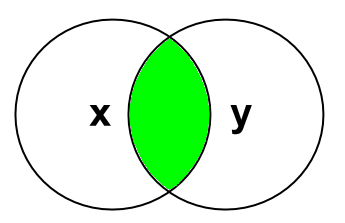
\includegraphics[width=1.73in]{images/inner_join}

\texttt{inner\_join(x,\ y)} only includes observations that match in
both x and y:

\begin{Shaded}
\begin{Highlighting}[]
\KeywordTok{inner_join}\NormalTok{(df1, df2)}
\end{Highlighting}
\end{Shaded}

\begin{verbatim}
## Joining, by = "id"
\end{verbatim}

\begin{verbatim}
##   id x1 x2
## 1  3  c  c
## 2  4  d  d
\end{verbatim}

\subsection{\texorpdfstring{\texttt{left\_join(x,\ y)}}{left\_join(x, y)}}\label{left_joinx-y}

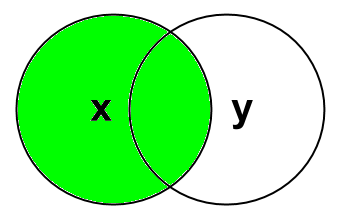
\includegraphics[width=1.7in]{images/left_join}

\texttt{left\_join(x,\ y)} includes all observations in \texttt{x},
regardless of whether they match or not. This is the most commonly used
join because it ensures that you don't lose observations from your
primary table:

\begin{Shaded}
\begin{Highlighting}[]
\KeywordTok{left_join}\NormalTok{(df1, df2)}
\end{Highlighting}
\end{Shaded}

\begin{verbatim}
## Joining, by = "id"
\end{verbatim}

\begin{verbatim}
##   id x1   x2
## 1  1  a <NA>
## 2  2  b <NA>
## 3  3  c    c
## 4  4  d    d
\end{verbatim}

\subsection{\texorpdfstring{\texttt{right\_join(x,\ y)}}{right\_join(x, y)}}\label{right_joinx-y}

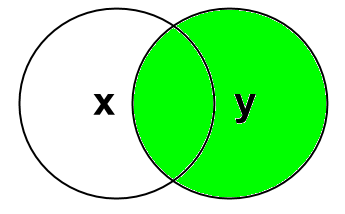
\includegraphics[width=1.73in]{images/right_join}

\texttt{right\_join(x,\ y)} includes all observations in \texttt{y}.
It's equivalent to \texttt{left\_join(y,\ x)}, but the columns will be
ordered differently:

\begin{Shaded}
\begin{Highlighting}[]
\KeywordTok{right_join}\NormalTok{(df1, df2)}
\end{Highlighting}
\end{Shaded}

\begin{verbatim}
## Joining, by = "id"
\end{verbatim}

\begin{verbatim}
##   id   x1 x2
## 1  3    c  c
## 2  4    d  d
## 3  5 <NA>  e
\end{verbatim}

\begin{Shaded}
\begin{Highlighting}[]
\KeywordTok{left_join}\NormalTok{(df2, df1)}
\end{Highlighting}
\end{Shaded}

\begin{verbatim}
## Joining, by = "id"
\end{verbatim}

\begin{verbatim}
##   id x2   x1
## 1  3  c    c
## 2  4  d    d
## 3  5  e <NA>
\end{verbatim}

\subsection{\texorpdfstring{\texttt{full\_join()}}{full\_join()}}\label{full_join}

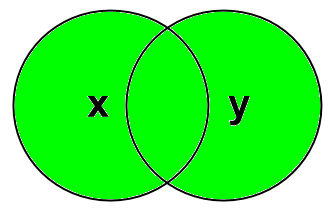
\includegraphics[width=1.68in]{images/full_join}

\texttt{full\_join()} includes all observations from \texttt{x} and
\texttt{y}:

\begin{Shaded}
\begin{Highlighting}[]
\KeywordTok{full_join}\NormalTok{(df1, df2)}
\end{Highlighting}
\end{Shaded}

\begin{verbatim}
## Joining, by = "id"
\end{verbatim}

\begin{verbatim}
##   id   x1   x2
## 1  1    a <NA>
## 2  2    b <NA>
## 3  3    c    c
## 4  4    d    d
## 5  5 <NA>    e
\end{verbatim}

The left, right and full joins are collectively know as outer joins.
When a row doesn't match in an outer join, the new variables are filled
in with missing values.

\chapter{Data Discovery with R}\label{data-discovery-with-r}

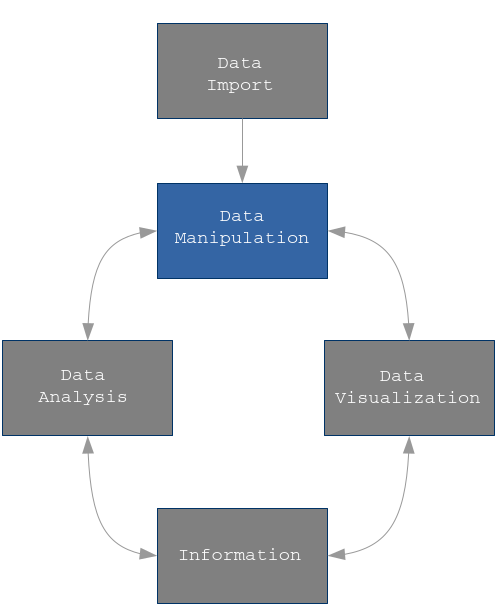
\includegraphics[width=3.33in]{images/flow-dtman}

\texttt{dplyr} provides also the tools for discovering your data. We are
talking about \texttt{summarise()} verb, which collapse many values into
a summary and about other best practices that allows us to combine
together multiple operations.

\begin{Shaded}
\begin{Highlighting}[]
\KeywordTok{require}\NormalTok{(dplyr)}
\end{Highlighting}
\end{Shaded}

In the following examples, we will refer to \texttt{bank} data set.

\begin{Shaded}
\begin{Highlighting}[]
\KeywordTok{require}\NormalTok{(qdata)}
\KeywordTok{data}\NormalTok{(bank)}
\NormalTok{bank}
\end{Highlighting}
\end{Shaded}

\begin{verbatim}
## # A tibble: 45,211 × 20
##       id   age          job  marital education default balance housing
##    <int> <int>       <fctr>   <fctr>    <fctr>  <fctr>   <int>  <fctr>
## 1      1    58   management  married  tertiary      no    2143     yes
## 2      2    44   technician   single secondary      no      29     yes
## 3      3    33 entrepreneur  married secondary      no       2     yes
## 4      4    47  blue-collar  married   unknown      no    1506     yes
## 5      5    33      unknown   single   unknown      no       1      no
## 6      6    35   management  married  tertiary      no     231     yes
## 7      7    28   management   single  tertiary      no     447     yes
## 8      8    42 entrepreneur divorced  tertiary     yes       2     yes
## 9      9    58      retired  married   primary      no     121     yes
## 10    10    43   technician   single secondary      no     593     yes
## # ... with 45,201 more rows, and 12 more variables: loan <fctr>,
## #   contact <fctr>, day <int>, month <fctr>, year <int>, date <dttm>,
## #   duration <int>, campaign <int>, pdays <int>, previous <int>,
## #   poutcome <fctr>, y <fctr>
\end{verbatim}

\section{\texorpdfstring{Descriptive statistics with
\texttt{summarise()} and
\texttt{group\_by()}}{Descriptive statistics with summarise() and group\_by()}}\label{descriptive-statistics-with-summarise-and-group_by}

\texttt{summarise()} collapses a data frame to a single row and allows
us to compute descriptive statistics. Let us see some examples:

\begin{Shaded}
\begin{Highlighting}[]
\CommentTok{# Compute the mean of balance of the accounts}
\KeywordTok{summarise}\NormalTok{(bank, }\DataTypeTok{mean_balance =} \KeywordTok{mean}\NormalTok{(balance, }\DataTypeTok{na.rm =} \OtherTok{TRUE}\NormalTok{))}
\end{Highlighting}
\end{Shaded}

\begin{verbatim}
## # A tibble: 1 × 1
##   mean_balance
##          <dbl>
## 1     1362.272
\end{verbatim}

\begin{Shaded}
\begin{Highlighting}[]
\CommentTok{# Compute the sum of balance of the accounts}
\NormalTok{bank %>%}\StringTok{ }\KeywordTok{summarise}\NormalTok{(}\DataTypeTok{max_balance =} \KeywordTok{sum}\NormalTok{(balance, }\DataTypeTok{na.rm =} \OtherTok{TRUE}\NormalTok{))}
\end{Highlighting}
\end{Shaded}

\begin{verbatim}
## # A tibble: 1 × 1
##   max_balance
##         <int>
## 1    61589682
\end{verbatim}

\begin{Shaded}
\begin{Highlighting}[]
\CommentTok{# Compute the minimum and the maximum balance of the accounts}
\NormalTok{bank %>%}\StringTok{ }\KeywordTok{summarise}\NormalTok{(}\DataTypeTok{max_balance =} \KeywordTok{max}\NormalTok{(balance, }\DataTypeTok{na.rm =} \OtherTok{TRUE}\NormalTok{), }\DataTypeTok{min_balance =} \KeywordTok{min}\NormalTok{(balance, }\DataTypeTok{na.rm =} \OtherTok{TRUE}\NormalTok{))}
\end{Highlighting}
\end{Shaded}

\begin{verbatim}
## # A tibble: 1 × 2
##   max_balance min_balance
##         <int>       <int>
## 1      102127       -8019
\end{verbatim}

\begin{Shaded}
\begin{Highlighting}[]
\CommentTok{# Compute the summary (number of obs, minimum, first quartile, median, mean, third quartile, }
\CommentTok{# maximum and standard deviation) of balance of the accounts  }
\NormalTok{bank %>%}\StringTok{ }\KeywordTok{summarise}\NormalTok{(}\DataTypeTok{n_obs =} \KeywordTok{n}\NormalTok{(),}
              \DataTypeTok{min=}\KeywordTok{min}\NormalTok{(balance, }\DataTypeTok{na.rm =} \OtherTok{TRUE}\NormalTok{),}
              \DataTypeTok{first_q=}\KeywordTok{quantile}\NormalTok{(balance, }\DataTypeTok{prob =} \FloatTok{0.25}\NormalTok{, }\DataTypeTok{na.rm =} \OtherTok{TRUE}\NormalTok{),}
              \DataTypeTok{median=}\KeywordTok{median}\NormalTok{(balance, }\DataTypeTok{na.rm =} \OtherTok{TRUE}\NormalTok{),}
              \DataTypeTok{mean=}\KeywordTok{mean}\NormalTok{(balance, }\DataTypeTok{na.rm =}\OtherTok{TRUE}\NormalTok{),}
              \DataTypeTok{third_q=}\KeywordTok{quantile}\NormalTok{(balance, }\DataTypeTok{prob =} \FloatTok{0.75}\NormalTok{, }\DataTypeTok{na.rm =} \OtherTok{TRUE}\NormalTok{),}
              \DataTypeTok{max=}\KeywordTok{max}\NormalTok{(balance, }\DataTypeTok{na.rm =} \OtherTok{TRUE}\NormalTok{),}
              \DataTypeTok{sd=}\KeywordTok{sd}\NormalTok{(balance, }\DataTypeTok{na.rm =}\OtherTok{TRUE}\NormalTok{))}
\end{Highlighting}
\end{Shaded}

\begin{verbatim}
## # A tibble: 1 × 8
##   n_obs   min first_q median     mean third_q    max       sd
##   <int> <int>   <dbl>  <int>    <dbl>   <dbl>  <int>    <dbl>
## 1 45211 -8019      72    448 1362.272    1428 102127 3044.766
\end{verbatim}

Descriptive statistics can be computed also by groups, by using
\texttt{group\_by()}, which is a \texttt{dplyr} function that allows us
to group observations according to the levels of a variable/s.

\begin{Shaded}
\begin{Highlighting}[]
\CommentTok{# Compute the mean of balance of the accounts by job}
\NormalTok{bank %>%}\StringTok{ }
\StringTok{  }\KeywordTok{group_by}\NormalTok{(job) %>%}
\StringTok{  }\KeywordTok{summarise}\NormalTok{(}\DataTypeTok{mean_balance =} \KeywordTok{mean}\NormalTok{(balance, }\DataTypeTok{na.rm =} \OtherTok{TRUE}\NormalTok{))}
\end{Highlighting}
\end{Shaded}

\begin{verbatim}
## # A tibble: 12 × 2
##              job mean_balance
##           <fctr>        <dbl>
## 1         admin.    1135.8389
## 2    blue-collar    1078.8267
## 3   entrepreneur    1521.4701
## 4      housemaid    1392.3952
## 5     management    1763.6168
## 6        retired    1984.2151
## 7  self-employed    1647.9709
## 8       services     997.0881
## 9        student    1388.0608
## 10    technician    1252.6321
## 11    unemployed    1521.7460
## 12       unknown    1772.3576
\end{verbatim}

\begin{Shaded}
\begin{Highlighting}[]
\CommentTok{# Compute the summary (number of obs, minimum, first quartile, median, mean, third quantile, }
\CommentTok{# maximum and standard deviation) of balance of the accounts by job }
\NormalTok{bank %>%}\StringTok{ }
\StringTok{  }\KeywordTok{group_by}\NormalTok{(job) %>%}
\StringTok{  }\KeywordTok{summarise}\NormalTok{(}\DataTypeTok{n_obs =} \KeywordTok{n}\NormalTok{(),}
            \DataTypeTok{min=}\KeywordTok{min}\NormalTok{(balance, }\DataTypeTok{na.rm =} \OtherTok{TRUE}\NormalTok{),}
            \DataTypeTok{first_q=}\KeywordTok{quantile}\NormalTok{(balance, }\DataTypeTok{prob =} \FloatTok{0.25}\NormalTok{, }\DataTypeTok{na.rm =} \OtherTok{TRUE}\NormalTok{),}
            \DataTypeTok{median=}\KeywordTok{median}\NormalTok{(balance, }\DataTypeTok{na.rm =} \OtherTok{TRUE}\NormalTok{),}
            \DataTypeTok{mean=}\KeywordTok{mean}\NormalTok{(balance, }\DataTypeTok{na.rm =}\OtherTok{TRUE}\NormalTok{),}
            \DataTypeTok{third_q=}\KeywordTok{quantile}\NormalTok{(balance, }\DataTypeTok{prob =} \FloatTok{0.75}\NormalTok{, }\DataTypeTok{na.rm =} \OtherTok{TRUE}\NormalTok{),}
            \DataTypeTok{max=}\KeywordTok{max}\NormalTok{(balance, }\DataTypeTok{na.rm =} \OtherTok{TRUE}\NormalTok{),}
            \DataTypeTok{sd=}\KeywordTok{sd}\NormalTok{(balance, }\DataTypeTok{na.rm =}\OtherTok{TRUE}\NormalTok{))}
\end{Highlighting}
\end{Shaded}

\begin{verbatim}
## # A tibble: 12 × 9
##              job n_obs   min first_q median      mean third_q    max
##           <fctr> <int> <int>   <dbl>  <dbl>     <dbl>   <dbl>  <int>
## 1         admin.  5171 -1601   63.00  396.0 1135.8389 1203.00  64343
## 2    blue-collar  9732 -8019   55.00  388.0 1078.8267 1203.00  66653
## 3   entrepreneur  1487 -2082   44.50  352.0 1521.4701 1341.00  59649
## 4      housemaid  1240 -1941   57.75  406.0 1392.3952 1382.75  45141
## 5     management  9458 -6847   98.00  572.0 1763.6168 1825.00 102127
## 6        retired  2264 -1598  164.50  787.0 1984.2151 2309.00  81204
## 7  self-employed  1579 -3313  120.00  526.0 1647.9709 1603.50  52587
## 8       services  4154 -2122   35.00  339.5  997.0881 1071.75  57435
## 9        student   938  -679  148.25  502.0 1388.0608 1579.75  24025
## 10    technician  7597 -2827   61.00  421.0 1252.6321 1327.00  45248
## 11    unemployed  1303 -1270   94.00  529.0 1521.7460 1603.50  44134
## 12       unknown   288  -295  170.75  677.0 1772.3576 2165.50  19706
## # ... with 1 more variables: sd <dbl>
\end{verbatim}

\section{Multiple operations}\label{multiple-operations}

You can also chain together multiple operations to achieve a complex
result. Let us have a look!

\begin{Shaded}
\begin{Highlighting}[]
\CommentTok{# Compute the mean of balance of the accounts and the number of obs by job for people not older than 40 years and }
\CommentTok{# sort the result in ascending order  }
\NormalTok{bank %>%}
\StringTok{  }\KeywordTok{filter}\NormalTok{(age <}\StringTok{ }\DecValTok{40}\NormalTok{) %>%}
\StringTok{  }\KeywordTok{group_by}\NormalTok{(job) %>%}
\StringTok{  }\KeywordTok{summarise}\NormalTok{(}\DataTypeTok{n_obs =}\KeywordTok{n}\NormalTok{(),}
            \DataTypeTok{mean_balance =} \KeywordTok{mean}\NormalTok{(balance, }\DataTypeTok{na.rm =} \OtherTok{TRUE}\NormalTok{)) %>%}
\StringTok{  }\KeywordTok{arrange}\NormalTok{(mean_balance)}
\end{Highlighting}
\end{Shaded}

\begin{verbatim}
## # A tibble: 12 × 3
##              job n_obs mean_balance
##           <fctr> <int>        <dbl>
## 1        retired    25     445.8800
## 2       services  2419     827.6701
## 3         admin.  2924     936.2401
## 4    blue-collar  5064     951.9682
## 5   entrepreneur   647    1153.1453
## 6     technician  4376    1198.5599
## 7      housemaid   363    1346.0992
## 8     unemployed   631    1355.1886
## 9  self-employed   820    1379.8793
## 10       student   924    1385.0801
## 11    management  5101    1548.9508
## 12       unknown    68    1777.5882
\end{verbatim}

\chapter{Data Visualization with R}\label{data-visualization-with-r}

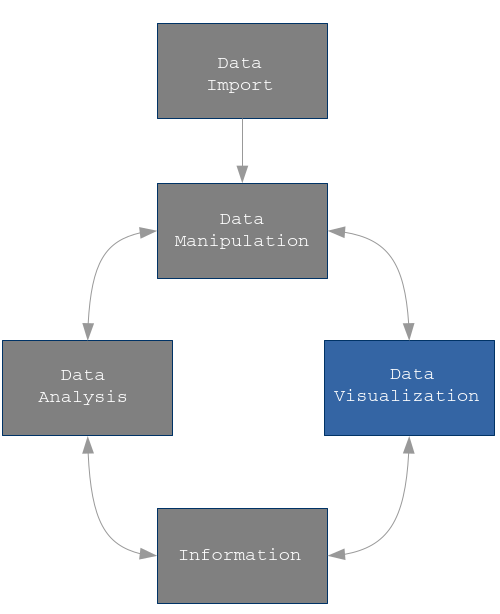
\includegraphics[width=3.33in]{images/flow-dtvisual}

Visualizing data is crucial in today's world. Without powerful
visualizations, it is almost impossible to create and narrate stories on
data. These stories help us build strategies and make intelligent
business decisions.

\texttt{ggplot2} is a data visualization package which has become a
synonym for data visualization in R.

\begin{Shaded}
\begin{Highlighting}[]
\KeywordTok{require}\NormalTok{(ggplot2)}
\end{Highlighting}
\end{Shaded}

Created by Hadley Wickham in 2005, \texttt{ggplot2} is an implementation
of Leland Wilkinson's Grammar of Graphics, a general scheme for data
visualization which breaks up graphs into semantic independent
components, such as scales and layers, that can be composed in many
different ways. This makes \texttt{ggplot2} very powerful, because there
are no limitations due to a set of pre-specified graphics, so it is
possible to create new graphics that are precisely tailored for the
problem in analysis.

\section{\texorpdfstring{An overview of \texttt{ggplot2}
grammar}{An overview of ggplot2 grammar}}\label{an-overview-of-ggplot2-grammar}

Let us consider \texttt{people} dataset, included in \texttt{qdata}
package. \texttt{people} dataset contains informations about weight,
height, gender and geographical area of 300 italian people.

\begin{Shaded}
\begin{Highlighting}[]
\KeywordTok{require}\NormalTok{(qdata)}
\end{Highlighting}
\end{Shaded}

Suppose we want to visualize the relationship between weight and height
of italian people according to the different geographical area, by using
a \textbf{scatterplot}:

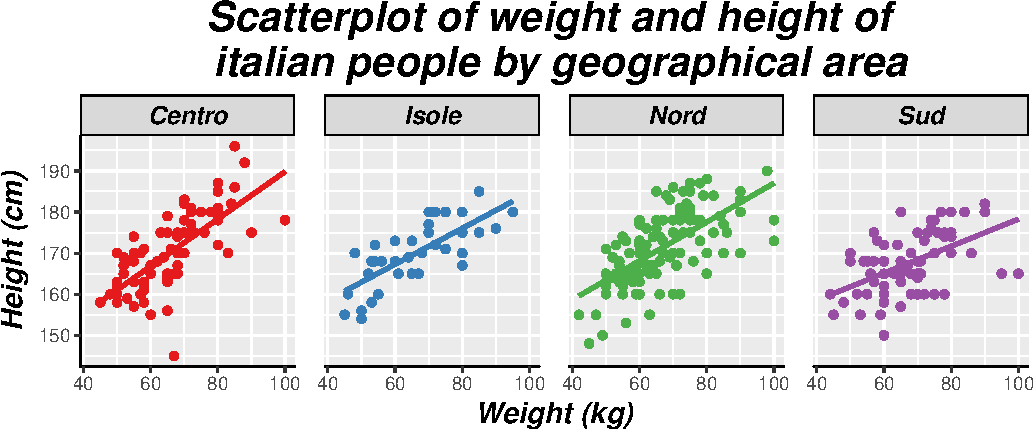
\includegraphics{09-data-visualization_files/figure-latex/complete_plot-1.pdf}

The previous plot is composed of building blocks that are added to the
plot one after the other.

The complete scheme of the most important building blocks of
\texttt{ggplot2} grammar is displayed in the following figure:

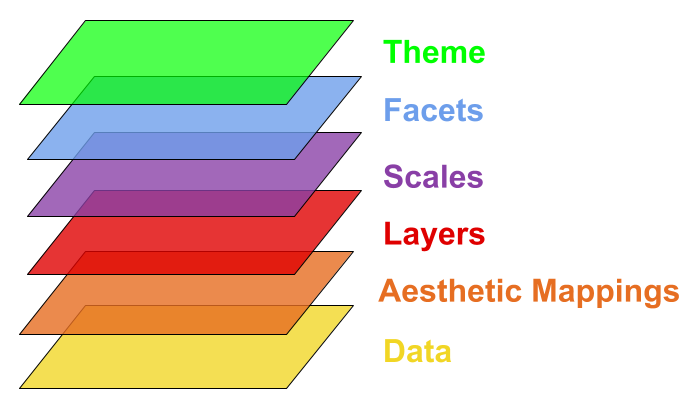
\includegraphics[width=4.63in]{images/schema-layer-ggplot2-mod}

The scheme must be read from bottom to top. Starting from bottom, the
first three building blocks ( {Data} , {Aestethic Mappings} and {Layers}
) are fundamental to build a simple plot, indeed they are called
\textbf{``key''} building blocks. The remaining building blocks (
{Scales} , {Coordinates} , {Facets} and {Themes} ) allow us to build a
complex plot and to customize it; their use and order is not compulsory.

Let us briefly describe the task of each element of the scheme and how
it helps build the previous plot:

\begin{enumerate}
\def\labelenumi{\arabic{enumi}.}
\tightlist
\item
   {Data} : the dataset that we want to visualize
\end{enumerate}


\includegraphics[width=3.43in]{images/schema-layer-ggplot2-data}

\begin{Shaded}
\begin{Highlighting}[]
\CommentTok{# people dataset}
\KeywordTok{data}\NormalTok{(people)}
\end{Highlighting}
\end{Shaded}

\begin{Shaded}
\begin{Highlighting}[]
\KeywordTok{head}\NormalTok{(people)}
\end{Highlighting}
\end{Shaded}

\begin{verbatim}
## # A tibble: 6 × 4
##   Gender   Area Weight Height
##   <fctr> <fctr>  <int>  <int>
## 1 Female  Isole     54    168
## 2 Female   Nord     61    171
## 3   Male    Sud     68    170
## 4 Female   Nord     52    164
## 5   Male   Nord     75    181
## 6   Male   Nord     77    178
\end{verbatim}

\begin{enumerate}
\def\labelenumi{\arabic{enumi}.}
\setcounter{enumi}{1}
\tightlist
\item
   {Aestethic Mappings} : describes how variables in the data are mapped
  to aestethic attributes that you can perceive
\end{enumerate}

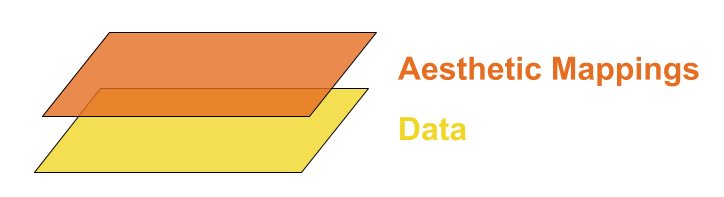
\includegraphics[width=4.83in]{images/schema-layer-ggplot2-aes}

\begin{longtable}[]{@{}llcc@{}}
\toprule
Gender & Area & Weight & Height\tabularnewline
\midrule
\endhead
& & x & y\tabularnewline
\bottomrule
\end{longtable}

\begin{Shaded}
\begin{Highlighting}[]
\KeywordTok{ggplot}\NormalTok{(}\DataTypeTok{data =} \NormalTok{people, }\KeywordTok{aes}\NormalTok{(}\DataTypeTok{x =} \NormalTok{Weight, }\DataTypeTok{y =} \NormalTok{Height))}
\end{Highlighting}
\end{Shaded}

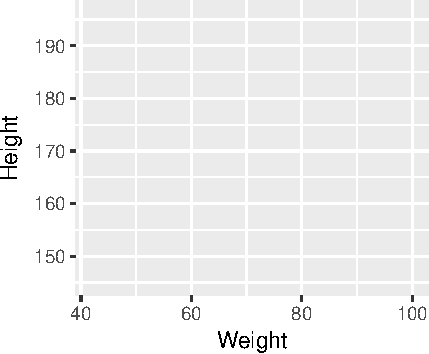
\includegraphics{09-data-visualization_files/figure-latex/aes-1.pdf}

\begin{enumerate}
\def\labelenumi{\arabic{enumi}.}
\setcounter{enumi}{2}
\tightlist
\item
   {Layers} : are made up by geometric elements and statistical
  transformations. In details, geometric objects (\texttt{geom}s)
  represent what we actually see on the plot: points, lines, polygons,
  etc. Statistical transformations (\texttt{stat}s) summarise data in
  many useful ways. For example, binning and counting observations to
  create an histogram, or summarising a 2d relationship with a linear
  model.
\end{enumerate}

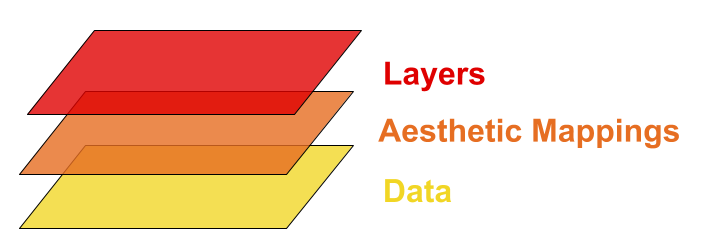
\includegraphics[width=4.72in]{images/schema-layer-ggplot2-layer}

\begin{Shaded}
\begin{Highlighting}[]
\CommentTok{# Scatterplot of the relationship between weight and height with regression line}
\KeywordTok{ggplot}\NormalTok{(people, }\KeywordTok{aes}\NormalTok{(}\DataTypeTok{x =} \NormalTok{Weight, }\DataTypeTok{y =} \NormalTok{Height)) +}
\StringTok{  }\KeywordTok{geom_point}\NormalTok{() +}\StringTok{ }\CommentTok{# layer 1 (draw points)}
\StringTok{  }\KeywordTok{stat_smooth}\NormalTok{(}\DataTypeTok{method =} \StringTok{"lm"}\NormalTok{, }\DataTypeTok{se =} \OtherTok{FALSE}\NormalTok{) }\CommentTok{# layer 2 (draw regression line) }
\end{Highlighting}
\end{Shaded}

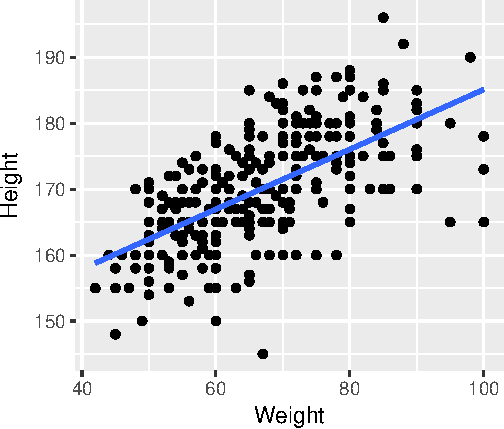
\includegraphics{09-data-visualization_files/figure-latex/layers-1.pdf}

\begin{enumerate}
\def\labelenumi{\arabic{enumi}.}
\setcounter{enumi}{3}
\tightlist
\item
   {Scales} : map values in the data space to values in an aesthetic
  space, whether it be colour, or size or shape. Scales draw a legend on
  axes, which provide an inverse mapping to make it possible to read the
  original data values from the graph. Scales are closely related to
  aestethics mapped.
\end{enumerate}

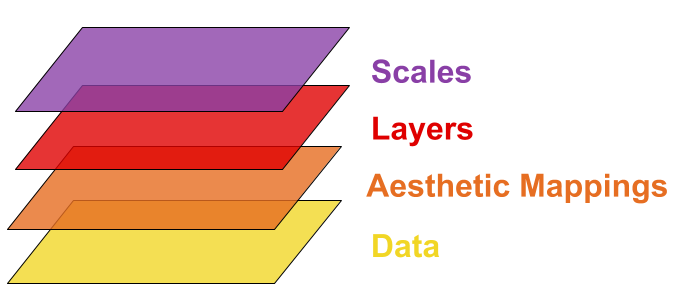
\includegraphics[width=4.61in]{images/schema-layer-ggplot2-scales}

\begin{Shaded}
\begin{Highlighting}[]
\CommentTok{# map Area to colour in aes() and change the default colours of colour scale  }
\KeywordTok{ggplot}\NormalTok{(people, }\KeywordTok{aes}\NormalTok{(}\DataTypeTok{x =} \NormalTok{Weight, }\DataTypeTok{y =} \NormalTok{Height, }\DataTypeTok{colour =} \NormalTok{Area)) +}
\StringTok{  }\KeywordTok{geom_point}\NormalTok{() +}
\StringTok{  }\KeywordTok{geom_smooth}\NormalTok{(}\DataTypeTok{method =} \StringTok{"lm"}\NormalTok{, }\DataTypeTok{se =} \OtherTok{FALSE}\NormalTok{) +}
\StringTok{  }\KeywordTok{scale_colour_brewer}\NormalTok{(}\DataTypeTok{palette=}\StringTok{"Set1"}\NormalTok{)}
\end{Highlighting}
\end{Shaded}

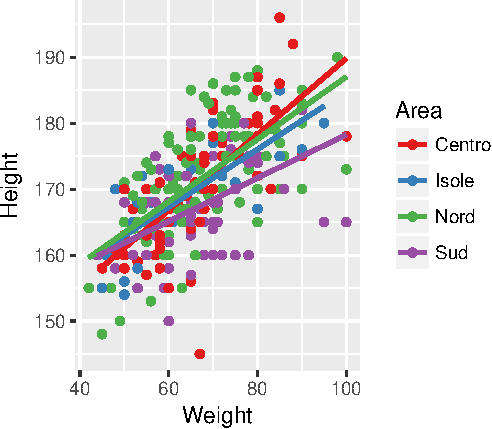
\includegraphics{09-data-visualization_files/figure-latex/scales-1.pdf}

\begin{enumerate}
\def\labelenumi{\arabic{enumi}.}
\setcounter{enumi}{4}
\tightlist
\item
   {Facets} : describes how to break up the data into subset and how to
  display those subsets as small multiples.
\end{enumerate}

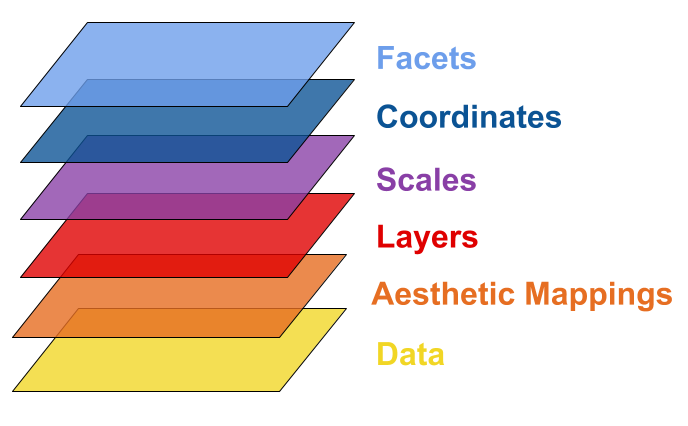
\includegraphics[width=4.61in]{images/schema-layer-ggplot2-facet}

\begin{Shaded}
\begin{Highlighting}[]
\CommentTok{# Generate a plot for each geographical area}
\KeywordTok{ggplot}\NormalTok{(people, }\KeywordTok{aes}\NormalTok{(}\DataTypeTok{x =} \NormalTok{Weight, }\DataTypeTok{y =} \NormalTok{Height, }\DataTypeTok{colour =} \NormalTok{Area)) +}
\StringTok{  }\KeywordTok{geom_point}\NormalTok{() +}
\StringTok{  }\KeywordTok{stat_smooth}\NormalTok{(}\DataTypeTok{method =} \StringTok{"lm"}\NormalTok{, }\DataTypeTok{se =} \OtherTok{FALSE}\NormalTok{) +}\StringTok{ }
\StringTok{  }\KeywordTok{scale_colour_brewer}\NormalTok{(}\DataTypeTok{palette=}\StringTok{"Set1"}\NormalTok{) +}
\StringTok{  }\KeywordTok{facet_grid}\NormalTok{(. ~}\StringTok{ }\NormalTok{Area)}
\end{Highlighting}
\end{Shaded}

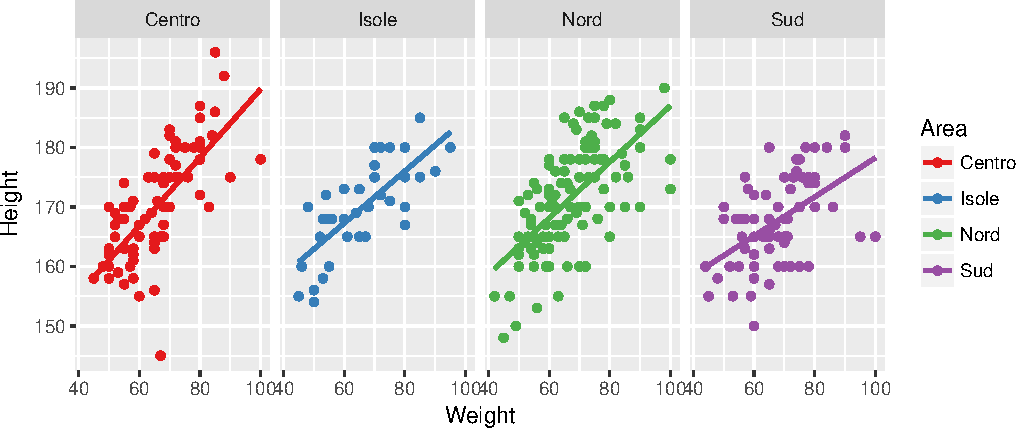
\includegraphics{09-data-visualization_files/figure-latex/facets-1.pdf}

\begin{enumerate}
\def\labelenumi{\arabic{enumi}.}
\setcounter{enumi}{5}
\tightlist
\item
   {Themes} : controls all non-data elements of the plot, like the font
  size, background colour, etc.
\end{enumerate}

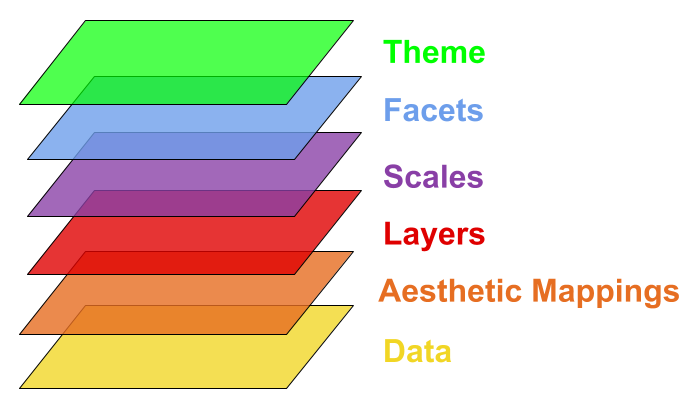
\includegraphics[width=4.63in]{images/schema-layer-ggplot2-mod}

\begin{Shaded}
\begin{Highlighting}[]
\CommentTok{# Customize the appearance of the plot}
\KeywordTok{ggplot}\NormalTok{(people, }\KeywordTok{aes}\NormalTok{(}\DataTypeTok{x =} \NormalTok{Weight, }\DataTypeTok{y =} \NormalTok{Height, }\DataTypeTok{colour =} \NormalTok{Area)) +}
\StringTok{  }\KeywordTok{geom_point}\NormalTok{() +}
\StringTok{  }\KeywordTok{stat_smooth}\NormalTok{(}\DataTypeTok{method =} \StringTok{"lm"}\NormalTok{, }\DataTypeTok{se =} \NormalTok{F) +}
\StringTok{  }\KeywordTok{scale_colour_brewer}\NormalTok{(}\DataTypeTok{palette=}\StringTok{"Set1"}\NormalTok{) +}
\StringTok{  }\KeywordTok{facet_grid}\NormalTok{(. ~}\StringTok{ }\NormalTok{Area) +}
\StringTok{  }\KeywordTok{ggtitle}\NormalTok{(}\StringTok{"Scatterplot of weight and height of }\CharTok{\textbackslash{}n}\StringTok{ italian people by geographical area"}\NormalTok{) +}\StringTok{ }
\StringTok{    }\KeywordTok{xlab}\NormalTok{(}\StringTok{"Weight (kg)"}\NormalTok{) +}
\StringTok{    }\KeywordTok{ylab}\NormalTok{(}\StringTok{"Height (cm)"}\NormalTok{) +}
\StringTok{  }\KeywordTok{theme}\NormalTok{(}\DataTypeTok{plot.background =} \KeywordTok{element_blank}\NormalTok{(),}
    \DataTypeTok{axis.line.x =} \KeywordTok{element_line}\NormalTok{(}\DataTypeTok{colour =} \StringTok{"black"}\NormalTok{),}
    \DataTypeTok{axis.line.y =} \KeywordTok{element_line}\NormalTok{(}\DataTypeTok{colour =} \StringTok{"black"}\NormalTok{),}
    \DataTypeTok{axis.title =} \KeywordTok{element_text}\NormalTok{(}\DataTypeTok{colour =} \StringTok{"black"}\NormalTok{, }\DataTypeTok{size =} \DecValTok{14}\NormalTok{, }\DataTypeTok{face =} \StringTok{"bold.italic"}\NormalTok{),}
    \DataTypeTok{strip.background =} \KeywordTok{element_rect}\NormalTok{(}\DataTypeTok{colour =} \StringTok{"black"}\NormalTok{),}
    \DataTypeTok{strip.text =} \KeywordTok{element_text}\NormalTok{(}\DataTypeTok{colour =} \StringTok{"black"}\NormalTok{, }\DataTypeTok{face =} \StringTok{"bold.italic"}\NormalTok{, }\DataTypeTok{size =} \DecValTok{12}\NormalTok{),}
    \DataTypeTok{plot.title =} \KeywordTok{element_text}\NormalTok{(}\DataTypeTok{colour =} \StringTok{"black"}\NormalTok{, }\DataTypeTok{size =} \DecValTok{20}\NormalTok{, }\DataTypeTok{face =} \StringTok{"bold.italic"}\NormalTok{, }\DataTypeTok{hjust =} \FloatTok{0.5}\NormalTok{),}
    \DataTypeTok{panel.spacing =} \KeywordTok{unit}\NormalTok{(}\DecValTok{1}\NormalTok{, }\StringTok{"lines"}\NormalTok{),}
    \DataTypeTok{legend.position=}\StringTok{"none"}\NormalTok{)}
\end{Highlighting}
\end{Shaded}

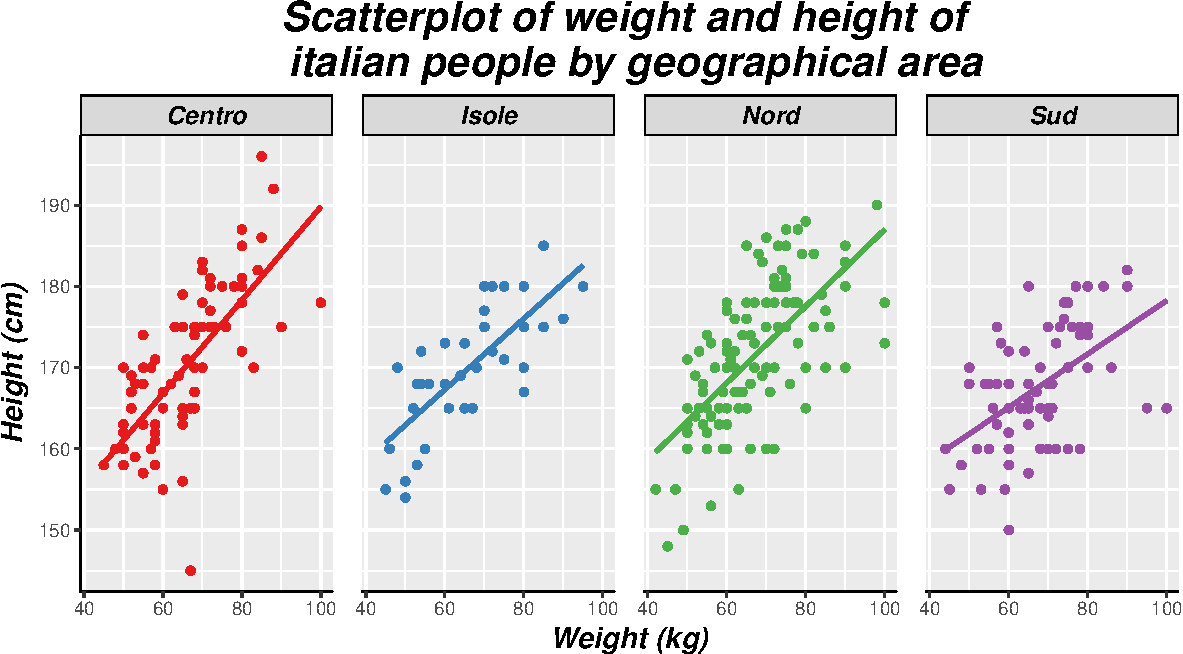
\includegraphics{09-data-visualization_files/figure-latex/theme-1.pdf}

\clearpage

\section{Other plot types}\label{other-plot-types}

The building block scheme previously seen can help us understanding how
to build other plot types. We will focus on the first three building
blocks of the scheme (data, aestethic mappings and layers).

\begin{itemize}
\tightlist
\item
  \textbf{Barplot}, which is used to show the count of each case of a
  categorial variable. Suppose we want to analyze the count of people by
  geographical area:
\end{itemize}

\begin{Shaded}
\begin{Highlighting}[]
\CommentTok{# base plot: key building blocks (data, aes, layer)}
\KeywordTok{ggplot}\NormalTok{(}\DataTypeTok{data =} \NormalTok{people, }\DataTypeTok{mapping =} \KeywordTok{aes}\NormalTok{(}\DataTypeTok{x =} \NormalTok{Area)) +}\StringTok{ }
\StringTok{  }\KeywordTok{geom_bar}\NormalTok{(}\DataTypeTok{fill =} \StringTok{"royalblue"}\NormalTok{, }\DataTypeTok{colour =} \StringTok{"black"}\NormalTok{, }\DataTypeTok{width =} \FloatTok{0.5}\NormalTok{)}
\end{Highlighting}
\end{Shaded}

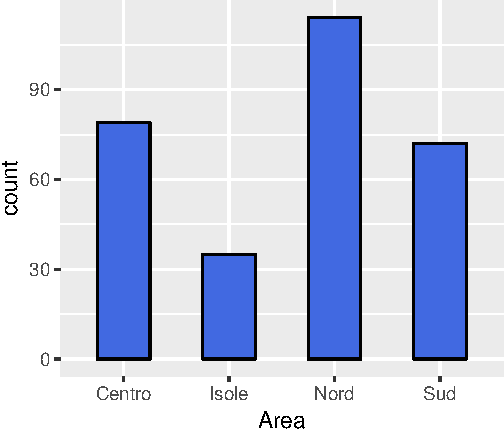
\includegraphics{09-data-visualization_files/figure-latex/barplot-1.pdf}

\begin{itemize}
\tightlist
\item
  \textbf{Histogram}, which is used to summarize a continuous variable
  into classes. Suppose we want to analyze the distribution of people
  weight:
\end{itemize}

\begin{Shaded}
\begin{Highlighting}[]
\CommentTok{# base plot: key building blocks (data, aes, layer)}
\KeywordTok{ggplot}\NormalTok{(}\DataTypeTok{data=}\NormalTok{people, }\DataTypeTok{mapping=}\KeywordTok{aes}\NormalTok{(}\DataTypeTok{x=}\NormalTok{Weight)) +}
\StringTok{  }\KeywordTok{geom_histogram}\NormalTok{(}\DataTypeTok{fill=}\StringTok{"#00cc66"}\NormalTok{, }\DataTypeTok{colour=} \StringTok{"#000000"}\NormalTok{, }\DataTypeTok{binwidth=}\DecValTok{5}\NormalTok{) }
\end{Highlighting}
\end{Shaded}

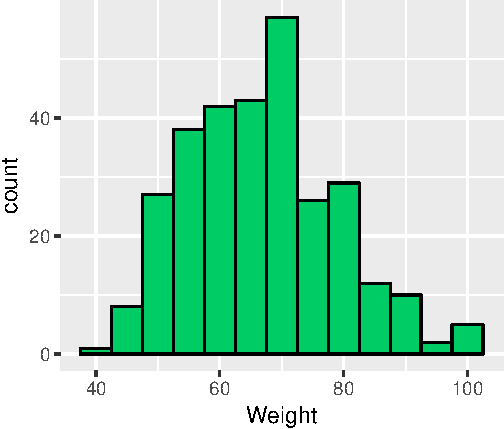
\includegraphics{09-data-visualization_files/figure-latex/histogram-1.pdf}

\clearpage

\begin{itemize}
\tightlist
\item
  \textbf{Boxplot}, which is used to draw a data distribution. Supposing
  you are interested in the differences of weight accordingly to
  geographical area:
\end{itemize}

\begin{Shaded}
\begin{Highlighting}[]
\CommentTok{# base plot: key building blocks (data, aes, layer)}
\KeywordTok{ggplot}\NormalTok{(}\DataTypeTok{data=}\NormalTok{people, }\KeywordTok{aes}\NormalTok{(}\DataTypeTok{x=}\NormalTok{Area, }\DataTypeTok{y=}\NormalTok{Weight)) +}\StringTok{ }
\StringTok{  }\KeywordTok{geom_boxplot}\NormalTok{(}\DataTypeTok{fill=}\StringTok{"#74a9cf"}\NormalTok{, }\DataTypeTok{colour=}\StringTok{"#034e7b"}\NormalTok{) }
\end{Highlighting}
\end{Shaded}

\includegraphics{09-data-visualization_files/figure-latex/boxplot-1.pdf}

\begin{itemize}
\tightlist
\item
  \textbf{Lineplot}, used to display how one continuous variable, on the
  y-axis, changes in relation to another continuous variable, on the
  x-axis. For this example we consider \texttt{orange} data, included in
  \texttt{qdata} package. \texttt{orange} contains information about the
  growth of 5 Orange Trees, according to their trunk circumferences.
\end{itemize}

\begin{Shaded}
\begin{Highlighting}[]
\KeywordTok{data}\NormalTok{(orange)}
\KeywordTok{head}\NormalTok{(orange)}
\end{Highlighting}
\end{Shaded}

\begin{verbatim}
##   Tree  age circumference
## 1    1  118            30
## 2    1  484            58
## 3    1  664            87
## 4    1 1004           115
## 5    1 1231           120
## 6    1 1372           142
\end{verbatim}

Suppose we want to represent the growth of one tree:

\begin{Shaded}
\begin{Highlighting}[]
\KeywordTok{require}\NormalTok{(dplyr)}
\CommentTok{# base plot of 1 tree: key components(data, aes, layer)}
\KeywordTok{ggplot}\NormalTok{(}\DataTypeTok{data=}\NormalTok{orange %>%}\StringTok{ }\KeywordTok{filter}\NormalTok{(Tree==}\DecValTok{1}\NormalTok{), }\DataTypeTok{mapping=}\KeywordTok{aes}\NormalTok{(}\DataTypeTok{x=}\NormalTok{age, }\DataTypeTok{y=}\NormalTok{circumference)) +}\StringTok{ }
\StringTok{  }\KeywordTok{geom_line}\NormalTok{(}\DataTypeTok{colour=} \StringTok{"#990033"}\NormalTok{, }\DataTypeTok{size=}\FloatTok{1.3}\NormalTok{)}
\end{Highlighting}
\end{Shaded}

\includegraphics{09-data-visualization_files/figure-latex/lineplot-1.pdf}

\chapter{Statistical Models with R}\label{statistical-models-with-r}

\includegraphics[width=3.33in]{images/flow-dtanal}

Data can be analysed by regression models with R. Regression is an
analysis that attempts to determine the strength of the relationship
between one dependent variable, \(y\), and a series of other changing
variables, \(x\).

There are lots of different types of regression models in statistics but
R mantains a coherent syntax for the estimation of all of them. Indeed,
the common interface to fit a model in R is made of a call to the
corresponding function with arguments \texttt{formula} and
\texttt{data}.

The \texttt{lm} and \texttt{aov} functions are used in R to fit
respectively linear regression and analysis of variance model and their
syntax is:

\begin{Shaded}
\begin{Highlighting}[]
\NormalTok{linear_model <-}\StringTok{ }\KeywordTok{lm}\NormalTok{(formula, data)}
\NormalTok{anova_model <-}\StringTok{ }\KeywordTok{aov}\NormalTok{(formula, data)}
\end{Highlighting}
\end{Shaded}

\texttt{formula} argument is a symbolic description of the model to be
fitted, which has the form:
\texttt{response\ variable\ ∼\ predictor\ variables}. The variables
involved in \texttt{formula} should be columns of a dataframe specified
in \texttt{data} argument.

The resulting object (\texttt{linear\_model} or \texttt{anova\_model})
is a list of elements containing information about regression results.
This information can be investigated by the following functions:

\begin{longtable}[]{@{}ll@{}}
\toprule
Expression & Description\tabularnewline
\midrule
\endhead
\texttt{coef(obj)} & regression coefficients\tabularnewline
\texttt{resid(obj)} & residuals\tabularnewline
\texttt{fitted(obj)} & fitted values\tabularnewline
\texttt{summary(obj)} & analysis summary\tabularnewline
\texttt{predict(obj,\ newdata\ =\ ndat)} & predict for
newdata\tabularnewline
\texttt{deviance(obj)} & residual sum of squares\tabularnewline
\bottomrule
\end{longtable}

Let us see an example of regression analysis.

\clearpage

\subsection{Drug Dosage and Reaction
Time}\label{drug-dosage-and-reaction-time}

In an experiment to investigate the effect of a depressant drug, the
reaction times of ten males rats to a certain stimulus were measured
after a specified dose of the drug had been administer to each rat. The
results were as follows:

\begin{Shaded}
\begin{Highlighting}[]
\KeywordTok{require}\NormalTok{(qdata)}
\KeywordTok{data}\NormalTok{(drug)}
\KeywordTok{str}\NormalTok{(drug)}
\end{Highlighting}
\end{Shaded}

\begin{verbatim}
## Classes 'tbl_df', 'tbl' and 'data.frame':    10 obs. of  3 variables:
##  $ rat : int  1 2 3 4 5 6 7 8 9 10
##  $ dose: num  0 0.1 0.2 0.3 0.4 0.5 0.6 0.7 0.8 0.9
##  $ time: num  0.32 0.24 0.4 0.52 0.44 0.56 0.64 0.52 0.6 0.8
\end{verbatim}

Basic graphical data exploration may be achieved with:

\begin{Shaded}
\begin{Highlighting}[]
\KeywordTok{require}\NormalTok{(ggplot2)}
\NormalTok{pl <-}\StringTok{ }\KeywordTok{ggplot}\NormalTok{(}\DataTypeTok{data =} \NormalTok{drug, }\DataTypeTok{mapping =} \KeywordTok{aes}\NormalTok{(}\DataTypeTok{x =} \NormalTok{dose, }\DataTypeTok{y=}\NormalTok{time)) +}\StringTok{ }
\StringTok{  }\KeywordTok{geom_point}\NormalTok{() +}
\StringTok{  }\KeywordTok{xlab}\NormalTok{(}\DataTypeTok{label =} \StringTok{"Dose (mg)"}\NormalTok{) +}
\StringTok{  }\KeywordTok{ylab}\NormalTok{(}\DataTypeTok{label =} \StringTok{"Reaction Time (secs)"}\NormalTok{)}

\NormalTok{pl}
\end{Highlighting}
\end{Shaded}

\includegraphics{10-statistical-models_files/figure-latex/drugplot-1.pdf}

A simple model for these data might be a straight line, which can be
easy superposed to the data scatterplot by:

\begin{Shaded}
\begin{Highlighting}[]
\NormalTok{pl +}\StringTok{ }\KeywordTok{geom_smooth}\NormalTok{(}\DataTypeTok{method=}\StringTok{"lm"}\NormalTok{, }\DataTypeTok{se=}\OtherTok{FALSE}\NormalTok{) }
\end{Highlighting}
\end{Shaded}

\includegraphics{10-statistical-models_files/figure-latex/reg-1.pdf}

The R command to fit a simple linear model is:

\begin{Shaded}
\begin{Highlighting}[]
\NormalTok{fm <-}\StringTok{ }\KeywordTok{lm}\NormalTok{(}\DataTypeTok{formula =} \NormalTok{time ~}\StringTok{ }\NormalTok{dose, }\DataTypeTok{data =} \NormalTok{drug)}
\end{Highlighting}
\end{Shaded}

As we said, \texttt{fm} object is a list of elements containing
information about regression results.

Regression results can be investigated by generic function
\texttt{summary()}, which includes the most important elements for model
interpretation.

\begin{Shaded}
\begin{Highlighting}[]
\KeywordTok{summary}\NormalTok{(fm)}
\end{Highlighting}
\end{Shaded}

\begin{verbatim}
## 
## Call:
## lm(formula = time ~ dose, data = drug)
## 
## Residuals:
##    Min     1Q Median     3Q    Max 
## -0.104 -0.064  0.024  0.056  0.088 
## 
## Coefficients:
##             Estimate Std. Error t value Pr(>|t|)    
## (Intercept)  0.28800    0.04522   6.368 0.000216 ***
## dose         0.48000    0.08471   5.666 0.000472 ***
## ---
## Signif. codes:  0 '***' 0.001 '**' 0.01 '*' 0.05 '.' 0.1 ' ' 1
## 
## Residual standard error: 0.07694 on 8 degrees of freedom
## Multiple R-squared:  0.8005, Adjusted R-squared:  0.7756 
## F-statistic: 32.11 on 1 and 8 DF,  p-value: 0.0004724
\end{verbatim}

Small p-values for t-test on coefficients lead to consider both
coefficients as significant. Adjust R-squared equal to 0.78 shows an
acceptable portion of total variation explained by the regression model.

Small p-value for F-statistic confirm fitted model significance when
compared with null model (model only with intercept).

You can also visualize single elements of \texttt{fm} list.\\
For example:

\begin{Shaded}
\begin{Highlighting}[]
\CommentTok{# regression coefficients}
\KeywordTok{coef}\NormalTok{(fm)}
\end{Highlighting}
\end{Shaded}

\begin{verbatim}
## (Intercept)        dose 
##       0.288       0.480
\end{verbatim}

\begin{Shaded}
\begin{Highlighting}[]
\CommentTok{# residuals}
\KeywordTok{resid}\NormalTok{(fm)}
\end{Highlighting}
\end{Shaded}

\begin{verbatim}
##      1      2      3      4      5      6      7      8      9     10 
##  0.032 -0.096  0.016  0.088 -0.040  0.032  0.064 -0.104 -0.072  0.080
\end{verbatim}

\begin{Shaded}
\begin{Highlighting}[]
\CommentTok{# fitted values}
\KeywordTok{fitted}\NormalTok{(fm)}
\end{Highlighting}
\end{Shaded}

\begin{verbatim}
##     1     2     3     4     5     6     7     8     9    10 
## 0.288 0.336 0.384 0.432 0.480 0.528 0.576 0.624 0.672 0.720
\end{verbatim}

Prediction for response variable at specific values of the explanatories
variable can be gained using \texttt{predict()} function with the
following sintax:

\begin{Shaded}
\begin{Highlighting}[]
\NormalTok{newdata <-}\StringTok{ }\KeywordTok{data.frame}\NormalTok{(}\DataTypeTok{dose =} \KeywordTok{c}\NormalTok{(}\FloatTok{0.2}\NormalTok{, }\FloatTok{0.4}\NormalTok{, }\FloatTok{0.6} \NormalTok{))}
\KeywordTok{predict} \NormalTok{(fm, }\DataTypeTok{newdata =} \NormalTok{newdata)}
\end{Highlighting}
\end{Shaded}

\begin{verbatim}
##     1     2     3 
## 0.384 0.480 0.576
\end{verbatim}

Note how the \texttt{newdata} argument within \texttt{predict()}
requires an object of class \texttt{data.frame}, whose column names have
to be equal to the explicative variables names of the model.

\clearpage

For a visual inspection of the suite of residuals plots of the model,
the sintax is:

\begin{Shaded}
\begin{Highlighting}[]
\KeywordTok{par}\NormalTok{(}\DataTypeTok{mfrow =} \KeywordTok{c}\NormalTok{(}\DecValTok{2}\NormalTok{,}\DecValTok{2}\NormalTok{))}
\KeywordTok{plot}\NormalTok{(fm)}
\end{Highlighting}
\end{Shaded}

\includegraphics{10-statistical-models_files/figure-latex/lmplot-1.pdf}

The ``Residuals vs Fitted'' plot does not show, in this example, any
particular pattern. The presence of patterns may suggest that the model
is inadequate. The ``Normal Q-Q'' plot shows points close to the
straight line. If the normal assumption of residuals is not satisfied,
points are far from the straight line. The ``Normal Q-Q plot'' is less
reliable on the distribution tails, i.e.~points ought be very far from
the straight line to suggest that residuals follow a non-normal
distribution. The ``Scale location'' is similar to the residuals versus
fitted values plot, but it uses the square root of the standardized
residuals in order to diminish skewness. Like the first plot, there
should be no discernable pattern to the plot. The ``Residuals vs
Leverage'' shows leverage points. Leverage points are those
observations, if any, made at extreme or outlying values of the
independent variables such that the lack of neighboring observations
means that the fitted regression model will pass close to that
particular observation. Leverage points fall out the dotted lines.

\chapter{Data Mining with R}\label{data-mining-with-r}

\includegraphics[width=3.33in]{images/flow-dtanal}

Data Mining is the process to discover interesting, previously unknown
and potentially useful information from large amounts of data. It is an
interdisciplinary field with contributions from many areas, such as
statistics, machine learning, information retrieval, pattern recognition
and bioinformatics. Data mining is widely used in many domains, such as
retail, finance, telecommunication and social media.

\includegraphics[width=12in]{images/DataMining}

R well supports data mining research and projects, providing lots of
packages for data minig techniques.

In this chapter we will analize Neural Networks, which is an advanced
data mining method.

\section{Neural Networks}\label{neural-networks}

Neural networks tries to artificially simulate the organization and
functioning of the human brain structures. A neural network can be seen
as a system capable of giving an answer to a question or provide an
output in response to an input. In particular, it takes a set of inputs
(explanatory variables), transforms and weights these within a set of
hidden units and hidden layers to produce a set of outputs or
predictions (that are also transformed).

Usually, neural networks are made up by three layers:

\begin{itemize}
\tightlist
\item
  input layer, that capture of the network input signals
\item
  hidden layer, that transform the inputs into something that the output
  layer can use
\item
  output layer, that produces output signals
\end{itemize}

Next figure is an example of a feed forward neural network consisting of
four inputs, a hidden layer that contains three units and an output
layer that contains two outputs. The outputs of nodes in one layer are
inputs to the next layer. The inputs to each node are combined using a
weighted linear combination. The result is then usually modified by a
nonlinear function before being output.

\includegraphics[width=4.77in]{images/nnet}

The R \texttt{nnet} package provides \texttt{nnet()} function, which
fits a single-hidden-layer neural network to data.

\begin{Shaded}
\begin{Highlighting}[]
\KeywordTok{require}\NormalTok{(nnet)}
\end{Highlighting}
\end{Shaded}

\texttt{nnet()} function syntax is very similar to the one used for
linear models:

\begin{Shaded}
\begin{Highlighting}[]
\NormalTok{nn_mod <-}\StringTok{ }\KeywordTok{nnet}\NormalTok{(formula, data, size)}
\end{Highlighting}
\end{Shaded}

\texttt{nnet()} function requires \texttt{formula} argument, which is a
symbolic description of the model to be fitted, which has the form:
\texttt{response\ variable\ ∼\ predictor\ variables}. The variables
involved in \texttt{formula} should be columns of a data frame specified
in \texttt{data} argument. Unlike linear model definiton, you have to
define \texttt{size} argument, which represents the number of units in
the hidden layer.

The resulting object is of \texttt{nnet} or \texttt{nnet.formula} class
and it can be investigated by most of the functions seen for linear
model like \texttt{summary()}, \texttt{predict()}, \texttt{coef()} and
\texttt{resid()}.

\subsection{Titanic}\label{titanic}

Let us see how Neural Network works, considering \texttt{titanic} data,
included in \texttt{qdata} package. \texttt{titanic} data contains
information about surviving to Titanic wreck along with personal and
travel information of the single passengers.

\begin{Shaded}
\begin{Highlighting}[]
\KeywordTok{require}\NormalTok{(qdata)}
\KeywordTok{data}\NormalTok{(titanic)}
\KeywordTok{head}\NormalTok{(titanic)}
\end{Highlighting}
\end{Shaded}

\begin{verbatim}
## # A tibble: 6 × 4
##    Class Gender   Age   Status
##   <fctr> <fctr> <int>   <fctr>
## 1  Coach Female    20 Survived
## 2  Coach Female    21 Survived
## 3  Coach Female    26 Survived
## 4  Coach Female    26     Died
## 5  Coach Female    36 Survived
## 6  Coach Female    41 Survived
\end{verbatim}

The aim of study is to find a prediction model to assess the probability
of die for each passenger based on its \texttt{Age}, \texttt{Gender},
and \texttt{Class} of accomodation.

Some tables could help in describing the relations between die
probability and explicative variables (\texttt{Age}, \texttt{Gender},
and \texttt{Class}):

\begin{Shaded}
\begin{Highlighting}[]
\KeywordTok{require}\NormalTok{(dplyr)}
\CommentTok{# frequency table of the counts and percentage of Died and Survived people }
\NormalTok{titanic %>%}\StringTok{ }
\StringTok{  }\KeywordTok{group_by}\NormalTok{(Status) %>%}
\StringTok{  }\KeywordTok{summarise}\NormalTok{(}\DataTypeTok{n =} \KeywordTok{n}\NormalTok{()) %>%}
\StringTok{  }\KeywordTok{mutate}\NormalTok{(}\DataTypeTok{freq =} \KeywordTok{paste}\NormalTok{(}\KeywordTok{round}\NormalTok{(n/}\KeywordTok{sum}\NormalTok{(n)*}\StringTok{ }\DecValTok{100}\NormalTok{, }\DecValTok{2}\NormalTok{), }\StringTok{"%"}\NormalTok{)) }
\end{Highlighting}
\end{Shaded}

\begin{verbatim}
## # A tibble: 2 × 3
##     Status     n   freq
##     <fctr> <int>  <chr>
## 1     Died  1490 67.7 %
## 2 Survived   711 32.3 %
\end{verbatim}

\begin{Shaded}
\begin{Highlighting}[]
\CommentTok{# frequency table of the counts and percentage of Died and Survived people by Class}
\NormalTok{titanic %>%}\StringTok{ }
\StringTok{  }\KeywordTok{group_by}\NormalTok{(Status, Class) %>%}
\StringTok{  }\KeywordTok{summarise}\NormalTok{(}\DataTypeTok{n =} \KeywordTok{n}\NormalTok{()) %>%}
\StringTok{  }\KeywordTok{mutate}\NormalTok{(}\DataTypeTok{freq =} \KeywordTok{paste}\NormalTok{(}\KeywordTok{round}\NormalTok{(n/}\KeywordTok{sum}\NormalTok{(n)*}\StringTok{ }\DecValTok{100}\NormalTok{, }\DecValTok{2}\NormalTok{), }\StringTok{"%"}\NormalTok{))}
\end{Highlighting}
\end{Shaded}

\begin{verbatim}
## Source: local data frame [4 x 4]
## Groups: Status [2]
## 
##     Status  Class     n    freq
##     <fctr> <fctr> <int>   <chr>
## 1     Died  Coach  1368 91.81 %
## 2     Died  First   122  8.19 %
## 3 Survived  Coach   508 71.45 %
## 4 Survived  First   203 28.55 %
\end{verbatim}

\begin{Shaded}
\begin{Highlighting}[]
\CommentTok{# frequency table of the counts and percentage of Died and Survived people by Gender}
\NormalTok{titanic %>%}\StringTok{ }
\StringTok{  }\KeywordTok{group_by}\NormalTok{(Status, Gender) %>%}
\StringTok{  }\KeywordTok{summarise}\NormalTok{(}\DataTypeTok{n=} \KeywordTok{n}\NormalTok{()) %>%}
\StringTok{  }\KeywordTok{mutate}\NormalTok{(}\DataTypeTok{freq =} \KeywordTok{paste}\NormalTok{(}\KeywordTok{round}\NormalTok{(n/}\KeywordTok{sum}\NormalTok{(n)*}\StringTok{ }\DecValTok{100}\NormalTok{, }\DecValTok{2}\NormalTok{), }\StringTok{"%"}\NormalTok{))}
\end{Highlighting}
\end{Shaded}

\begin{verbatim}
## Source: local data frame [4 x 4]
## Groups: Status [2]
## 
##     Status Gender     n    freq
##     <fctr> <fctr> <int>   <chr>
## 1     Died Female   126  8.46 %
## 2     Died   Male  1364 91.54 %
## 3 Survived Female   344 48.38 %
## 4 Survived   Male   367 51.62 %
\end{verbatim}

The above tables show counts and percentages of died and survived for
each combination of Sex and Class factors. Some relations appear, but
its interpretation is not really simple.

The following graph shows if some relations exist between Status and
Age:

\begin{Shaded}
\begin{Highlighting}[]
\KeywordTok{require}\NormalTok{(ggplot2)}
\KeywordTok{ggplot}\NormalTok{(}\DataTypeTok{data=}\NormalTok{titanic, }\DataTypeTok{mapping=}\KeywordTok{aes}\NormalTok{(}\DataTypeTok{x=}\NormalTok{Status, }\DataTypeTok{y=}\NormalTok{Age)) +}
\StringTok{  }\KeywordTok{geom_boxplot}\NormalTok{(}\DataTypeTok{fill=}\StringTok{"#74a9cf"}\NormalTok{, }\DataTypeTok{colour=}\StringTok{"#034e7b"}\NormalTok{)+}\StringTok{ }
\StringTok{  }\KeywordTok{ggtitle}\NormalTok{(}\StringTok{"Box-plot of Age within levels of Status"}\NormalTok{)}
\end{Highlighting}
\end{Shaded}

\includegraphics{11-data-mining_files/figure-latex/plot_status_age-1.pdf}

Apparently, a slightly lower age is in survived passengers.

Neural Network method allows us to assess the probability of die for
each passenger based on its \texttt{Age}, \texttt{Gender} and
\texttt{Class} of accomodation.

Let us divide the data in train and test samples in order to estimate
the model on train sample and to test the results on test sample.

\begin{Shaded}
\begin{Highlighting}[]
\CommentTok{# generate train and test sample }
\NormalTok{train <-}\StringTok{ }\NormalTok{titanic %>%}\StringTok{ }\KeywordTok{sample_frac}\NormalTok{(}\FloatTok{0.7}\NormalTok{)}
\NormalTok{test <-}\StringTok{ }\NormalTok{titanic %>%}\StringTok{ }\KeywordTok{slice}\NormalTok{(-}\KeywordTok{as.numeric}\NormalTok{(}\KeywordTok{rownames}\NormalTok{(train)))}
\end{Highlighting}
\end{Shaded}

Neural Network model estimate on train sample:

\begin{Shaded}
\begin{Highlighting}[]
\NormalTok{nn_mod <-}\StringTok{ }\KeywordTok{nnet}\NormalTok{(Status ~}\StringTok{ }\NormalTok{Class +}\StringTok{ }\NormalTok{Gender +}\StringTok{ }\NormalTok{Age, }\DataTypeTok{data =} \NormalTok{train, }\DataTypeTok{size =} \DecValTok{3}\NormalTok{)}
\end{Highlighting}
\end{Shaded}

\begin{verbatim}
## # weights:  16
## initial  value 1206.184649 
## iter  10 value 856.416481
## iter  20 value 781.747292
## iter  30 value 780.314962
## final  value 780.312829 
## converged
\end{verbatim}

The predictions on test sample can be gained using \texttt{predict()}
function:

\begin{Shaded}
\begin{Highlighting}[]
\NormalTok{pr <-}\StringTok{ }\KeywordTok{predict}\NormalTok{(}\DataTypeTok{object =} \NormalTok{nn_mod, }\DataTypeTok{newdata =} \NormalTok{test)}
\KeywordTok{head}\NormalTok{(pr)}
\end{Highlighting}
\end{Shaded}

\begin{verbatim}
##        [,1]
## 1 0.6778630
## 2 0.6778630
## 3 0.6778630
## 4 0.6778630
## 5 0.6778630
## 6 0.6753988
\end{verbatim}

The predictions included the probability of survive in the Titanic wreck
according to \texttt{Gender}, \texttt{Age} and \texttt{Class}. We define
that probabilities below 0.5 represent \texttt{Died} (\texttt{TRUE}) and
probabilities over 0.5 represent \texttt{Survived} (\texttt{FALSE}).

\begin{Shaded}
\begin{Highlighting}[]
\NormalTok{test <-}\StringTok{ }\NormalTok{test %>%}\StringTok{ }\KeywordTok{mutate}\NormalTok{(}\DataTypeTok{pr_mod =} \NormalTok{pr <}\StringTok{ }\NormalTok{.}\DecValTok{5}\NormalTok{)}
\end{Highlighting}
\end{Shaded}

Let us see how the performance of the fitted model on the test sample:

\begin{Shaded}
\begin{Highlighting}[]
\NormalTok{test %>%}\StringTok{ }
\StringTok{  }\KeywordTok{group_by}\NormalTok{(Status, pr_mod) %>%}
\StringTok{  }\KeywordTok{summarise}\NormalTok{(}\DataTypeTok{n =} \KeywordTok{n}\NormalTok{()) %>%}
\StringTok{  }\KeywordTok{mutate}\NormalTok{(}\DataTypeTok{freq =} \KeywordTok{paste}\NormalTok{(}\KeywordTok{round}\NormalTok{(n/}\KeywordTok{sum}\NormalTok{(n)*}\StringTok{ }\DecValTok{100}\NormalTok{, }\DecValTok{2}\NormalTok{), }\StringTok{"%"}\NormalTok{))}
\end{Highlighting}
\end{Shaded}

\begin{verbatim}
## Source: local data frame [4 x 4]
## Groups: Status [2]
## 
##     Status pr_mod     n    freq
##     <fctr>  <lgl> <int>   <chr>
## 1     Died  FALSE    81  16.1 %
## 2     Died   TRUE   422  83.9 %
## 3 Survived  FALSE    69 43.95 %
## 4 Survived   TRUE    88 56.05 %
\end{verbatim}

We conclude that the model has quite good performance in the prediction
of the probability of die in the Titanic wreck according to
\texttt{Gender}, \texttt{Age} and \texttt{Class}.

\chapter{Reports with R Markdown}\label{reports-with-r-markdown}

\includegraphics[width=4.08in]{./images/flow-info}

R Markdown provides an authoring framework for data science. R Markdown
allows us to turn our analysis into high quality documents, reports,
presentations and dashboards.

\clearpage

We can use a single R Markdown file to both:

\begin{itemize}
\tightlist
\item
  save and execute code
\item
  generate high quality reports that can be shared with an audience
\end{itemize}

R Markdown documents are fully reproducible and support multiple
programming languages like: R, Python, and SQL. It support also dozens
of static and dynamic output formats, including HTML, PDF, MS Word,
Beamer, HTML5 slides, Tufte-style handouts, books, dashboards, shiny
applications, scientific articles, websites, and more.

\section{Installation}\label{installation}

You can install the R Markdown package from CRAN as follows:

\begin{Shaded}
\begin{Highlighting}[]
\KeywordTok{install.packages}\NormalTok{(}\StringTok{"rmarkdown"}\NormalTok{)}
\end{Highlighting}
\end{Shaded}

\section{Markdown Basics}\label{markdown-basics}

This is an R Markdown file, a plain text file that has the extension
\texttt{.Rmd}:

\includegraphics[width=18cm]{images/rmd-1.png}

Notice that the file contains three types of content:

\begin{itemize}
\tightlist
\item
  An (optional) YAML header surrounded by \texttt{-\/-\/-}
\item
  R code chunks surrounded by \texttt{```}
\item
  text mixed with simple text formatting
\end{itemize}

Markdown is a simple formatting language designed to make authoring
content easy for everyone. Rather than writing complex markup code
(e.g.~HTML or LaTeX), Markdown enables the use of a syntax much more
like plain-text email.

\subsection{Basic rules for text}\label{basic-rules-for-text}

This section provides quick references to the most commonly used R
Markdown syntax.

\includegraphics[width=14cm]{images/rmd-cheatsheet.png}

\section{Rendering Output}\label{rendering-output}

To generate a report from the file, run the \texttt{render} command:

\begin{Shaded}
\begin{Highlighting}[]
\KeywordTok{require}\NormalTok{(rmarkdown)}
\KeywordTok{render}\NormalTok{(}\StringTok{"example.Rmd"}\NormalTok{)}
\end{Highlighting}
\end{Shaded}

Otherwise, use the ``Knit'' button in the RStudio IDE to render the file
and preview the output with a single click or the keyboard shortcut
\emph{Ctrl + Shift + K}.

\includegraphics[width=18cm]{images/rmd-3.png}

R Markdown generates a new file that contains selected text, code, and
results from the .Rmd file. The new file can be a finished web page,
PDF, MS Word document, slide show, notebook, handout, book, dashboard,
package vignette or other format.


\end{document}
